\documentclass[a4paper,10pt]{article}
\usepackage{beamerarticle}
\setjobnamebeamerversion{boot-b}

\usepackage{fullpage}

\usepackage[backend=biber,url=false,style=alphabetic]{biblatex}
\addbibresource{os.bib}

\usepackage{hyperref}
\usepackage[textsize=footnotesize]{todonotes}
\addtolength{\oddsidemargin}{-15pt}
\addtolength{\marginparsep}{5pt}
% \setlength{\marginparwidth}{1.2in}
% \let\oldmarginpar\marginpar
% \renewcommand\marginpar[1]{\-\oldmarginpar[\raggedleft\footnotesize #1]%
% {\raggedright\footnotesize #1}}
\newcommand{\Marginpar}[1]{\marginpar{\raggedright{\footnotesize \emph{#1}}}}

% http://tex.stackexchange.com/q/25259/86
% for *notes*
\defbeamertemplate<article>{frame begin}{lined}{
  \par\noindent\rule{\textwidth}{2pt}\par}
\defbeamertemplate<article>{frame end}{lined}{
  \par\vspace{1em}\noindent\rule{.1\textwidth}{.3pt}
  \raisebox{-3pt}{{\large \Info}}
  \rule{.1618\textwidth}{.3pt}\par\vspace{.5em}}

\setbeamertemplate{frame begin}[lined]
\setbeamertemplate{frame end}[lined]

%\documentclass[10pt,ignorenonframetext,xcolor=svgnames,hyperref={xetex,colorlinks,linkcolor=blue},compress]{beamer}

\usepackage{latexsym,pifont,units,amsmath,amsfonts,amssymb,marvosym}
\usepackage{xltxtra} %fontspec,xunicode are loaded here.
\defaultfontfeatures{Mapping=tex-text}
\setsansfont{DejaVu Sans}
\setmainfont{DejaVu Serif}

% \usepackage{graphicx} % beamer loads graphicx already.
\graphicspath{{./figs/}{../figs/}{./}{../}} %note that the trailing “/” is required

\usepackage{tikz}
\usetikzlibrary{arrows,decorations.pathmorphing,backgrounds,positioning,fit}

\usepackage{multicol,varwidth}

\usepackage{minted}
\renewcommand{\theFancyVerbLine}{
  \textcolor{lightgray}{\scriptsize \arabic{FancyVerbLine}}}

\newminted{gas}{ linenos=true,numbersep=2pt,fontsize=\footnotesize,
  frame=leftline,framesep=3pt,rulecolor=\color{lightgray}, xleftmargin=10pt }
\newminted{c}{ linenos=true,numbersep=2pt,fontsize=\footnotesize,
  frame=leftline,framesep=3pt,rulecolor=\color{lightgray}, xleftmargin=10pt }

\newcommand{\cfbox}[2]{%
  \colorlet{currentcolor}{.}%
  {\color{#1}\fbox{\color{currentcolor}#2}}%
}

\newcommand{\code}[1]{\texttt{\textcolor{violet}{#1}}}

\mode<beamer>{
  \usetheme{default}
  \usecolortheme{sidebartab}
  \usefonttheme{serif}
  \setbeamertemplate{footline}[frame number]
  \setbeamertemplate{navigation symbols}{}
  \usenavigationsymbolstemplate{}
  \setbeamertemplate{blocks}[rounded][shadow=true]
  \setbeamercolor{structure}{fg=Green}
  \setbeamercolor{block title}{fg=Green}
}

\begin{document}

\mode<article>{
  \title{From Power Up To Bash Prompt}
  \author{Wang Xiaolin\\wx672ster@gmail.com}
  \maketitle
  \tableofcontents
  \vspace{2em}
  \begin{description}
  \item[Textbook:]\
    \begin{itemize}
    \item Appendix A, \emph{System Startup}, \cite{bovet2005understanding}
    \item Appendix D, \emph{System Startup}, \cite{mauerer2008professional}
    \item Chapter 8, \emph{Booting the Kernel}, \cite{rodriguez2005linux}
    \end{itemize}
  \end{description}
  \printbibliography
  \clearpage
}

\begin{frame}<beamer>
    \title{From Power Up To Bash Prompt}
    \author{Wang Xiaolin}
    \titlepage
    \vfill
    \tiny{
      \ding{41} wx672ster+os@gmail.com
      % \ding{37} 13577067397
    }
\end{frame}

\section{Motherboard Chipsets And The Memory Map}
\label{sec:moth-chips-memory}

See \cite{gustavo2008chipsets}

\begin{frame}{Motherboard Chipsets And The Memory Map}
  \begin{center}
    \mode<beamer>{
      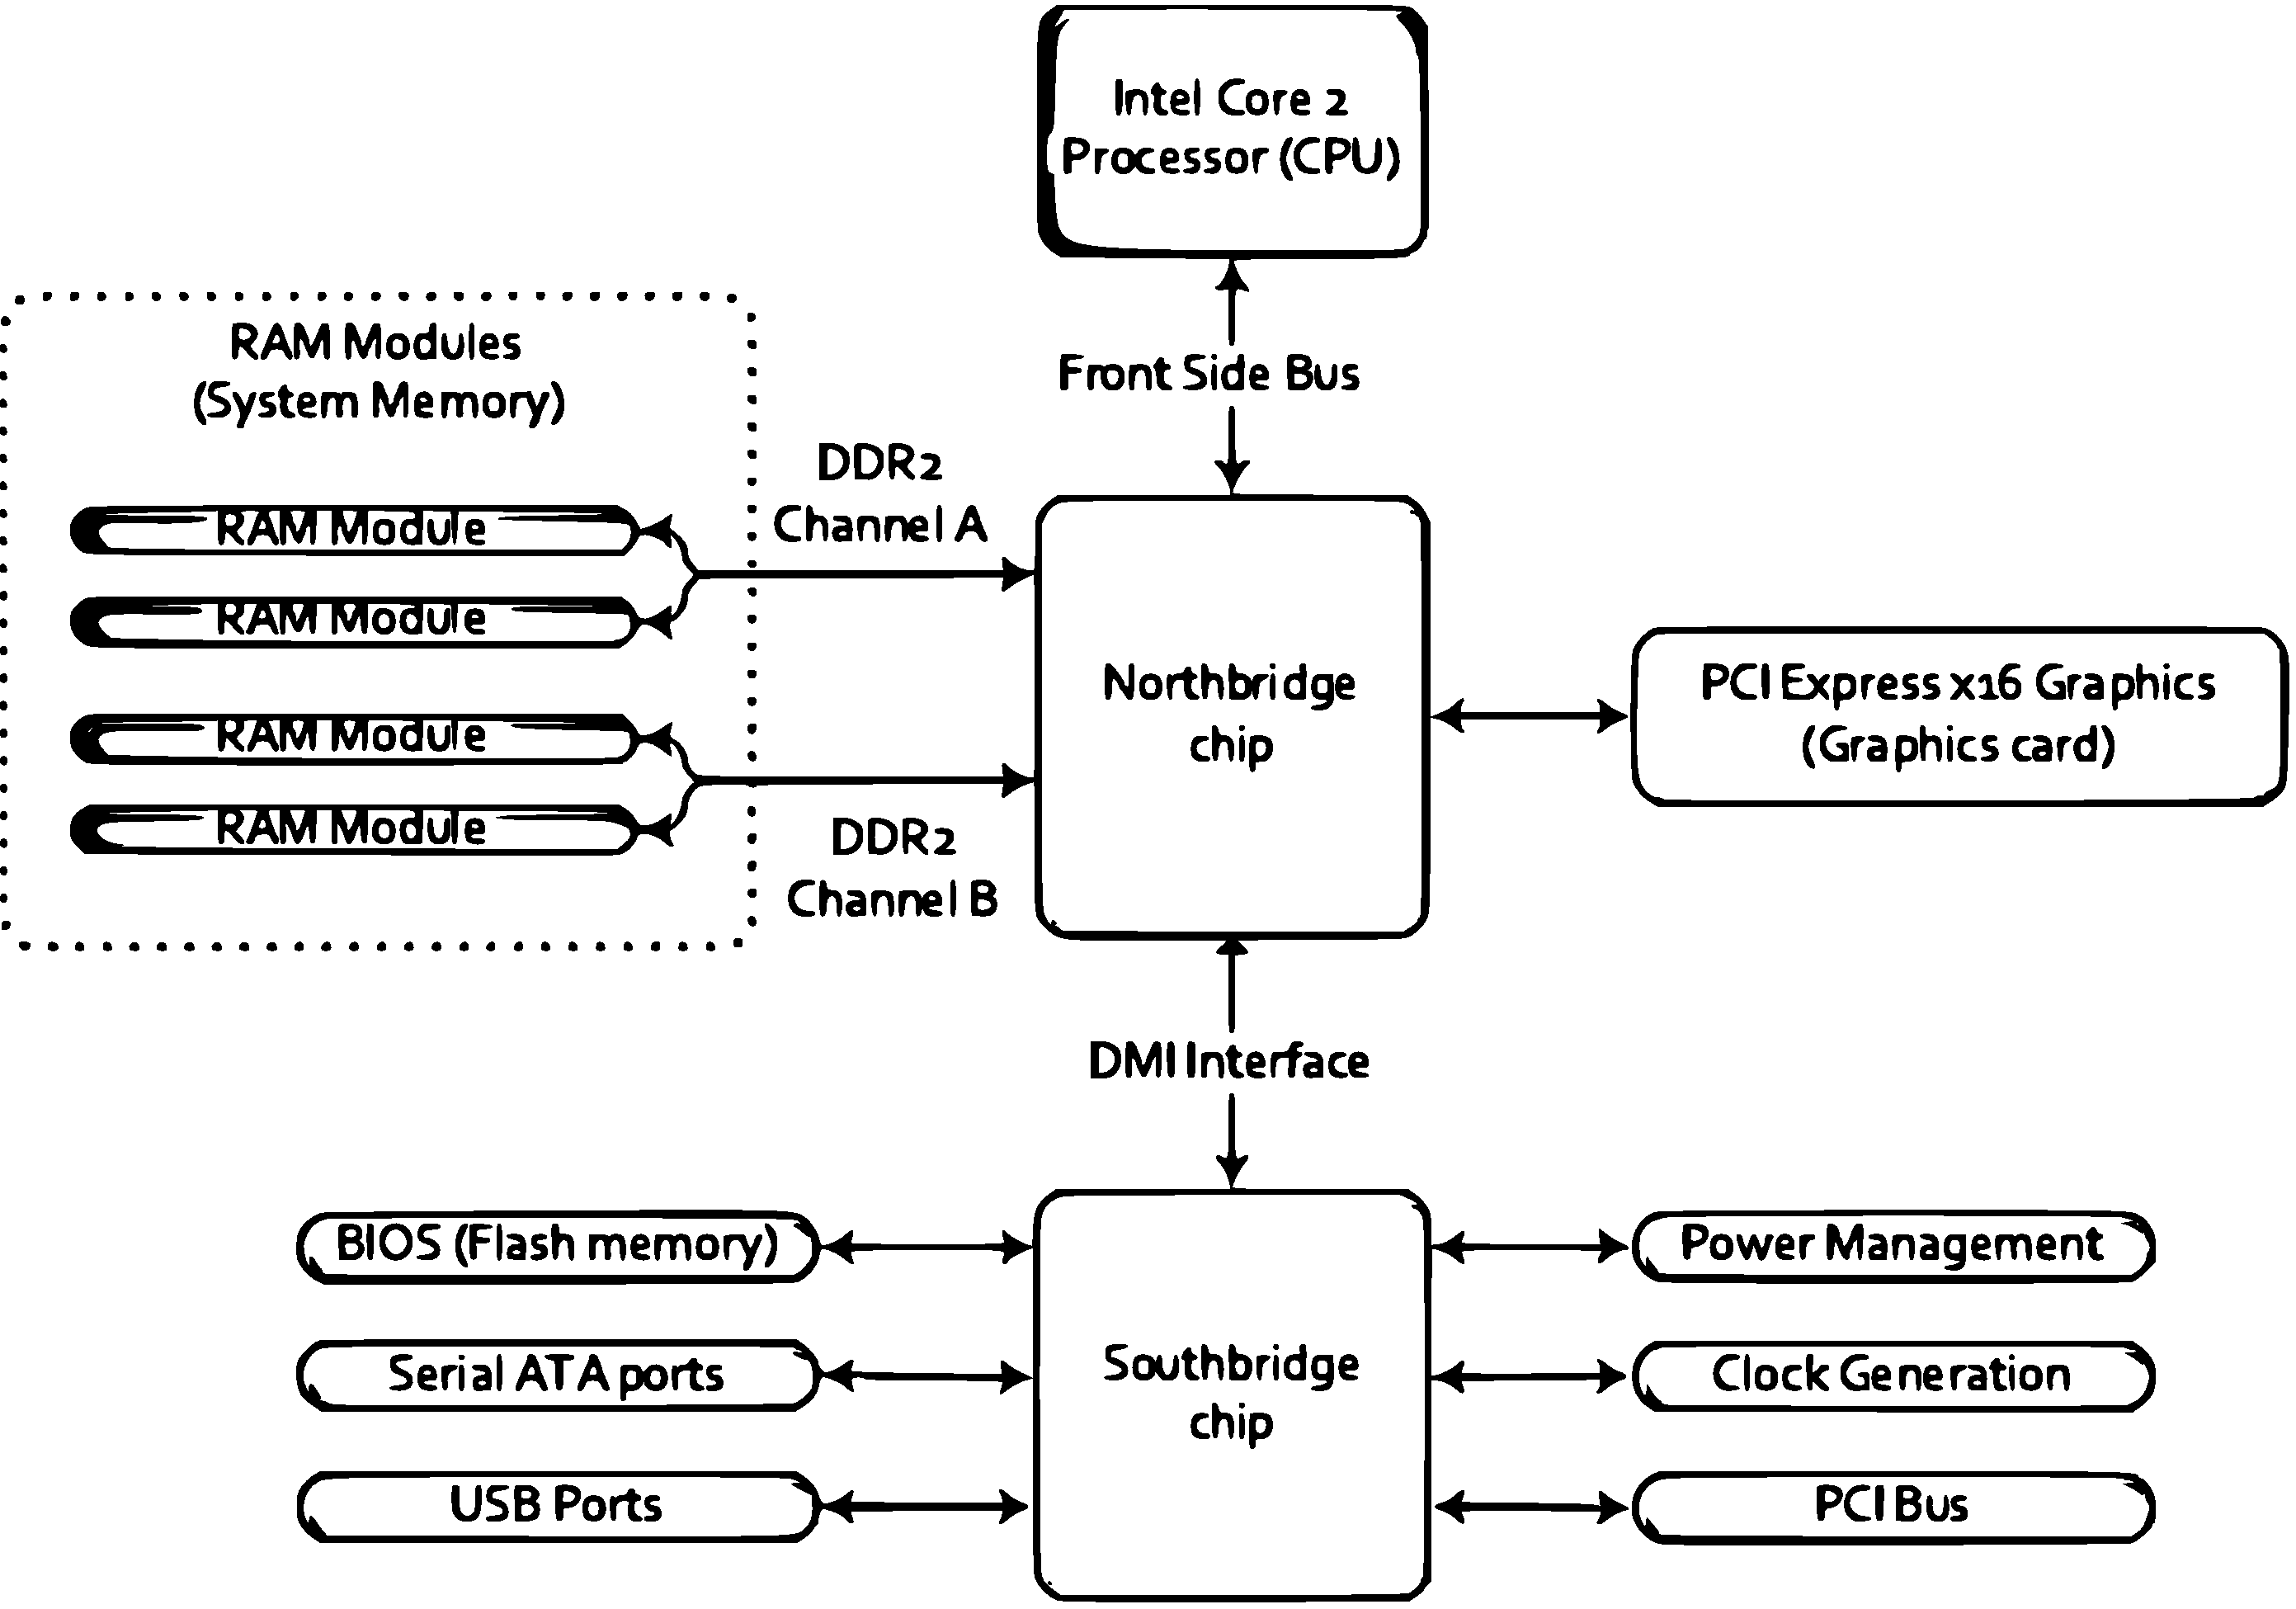
\includegraphics[width=\textwidth]{motherboardDiagram}
    }
    \mode<article>{
      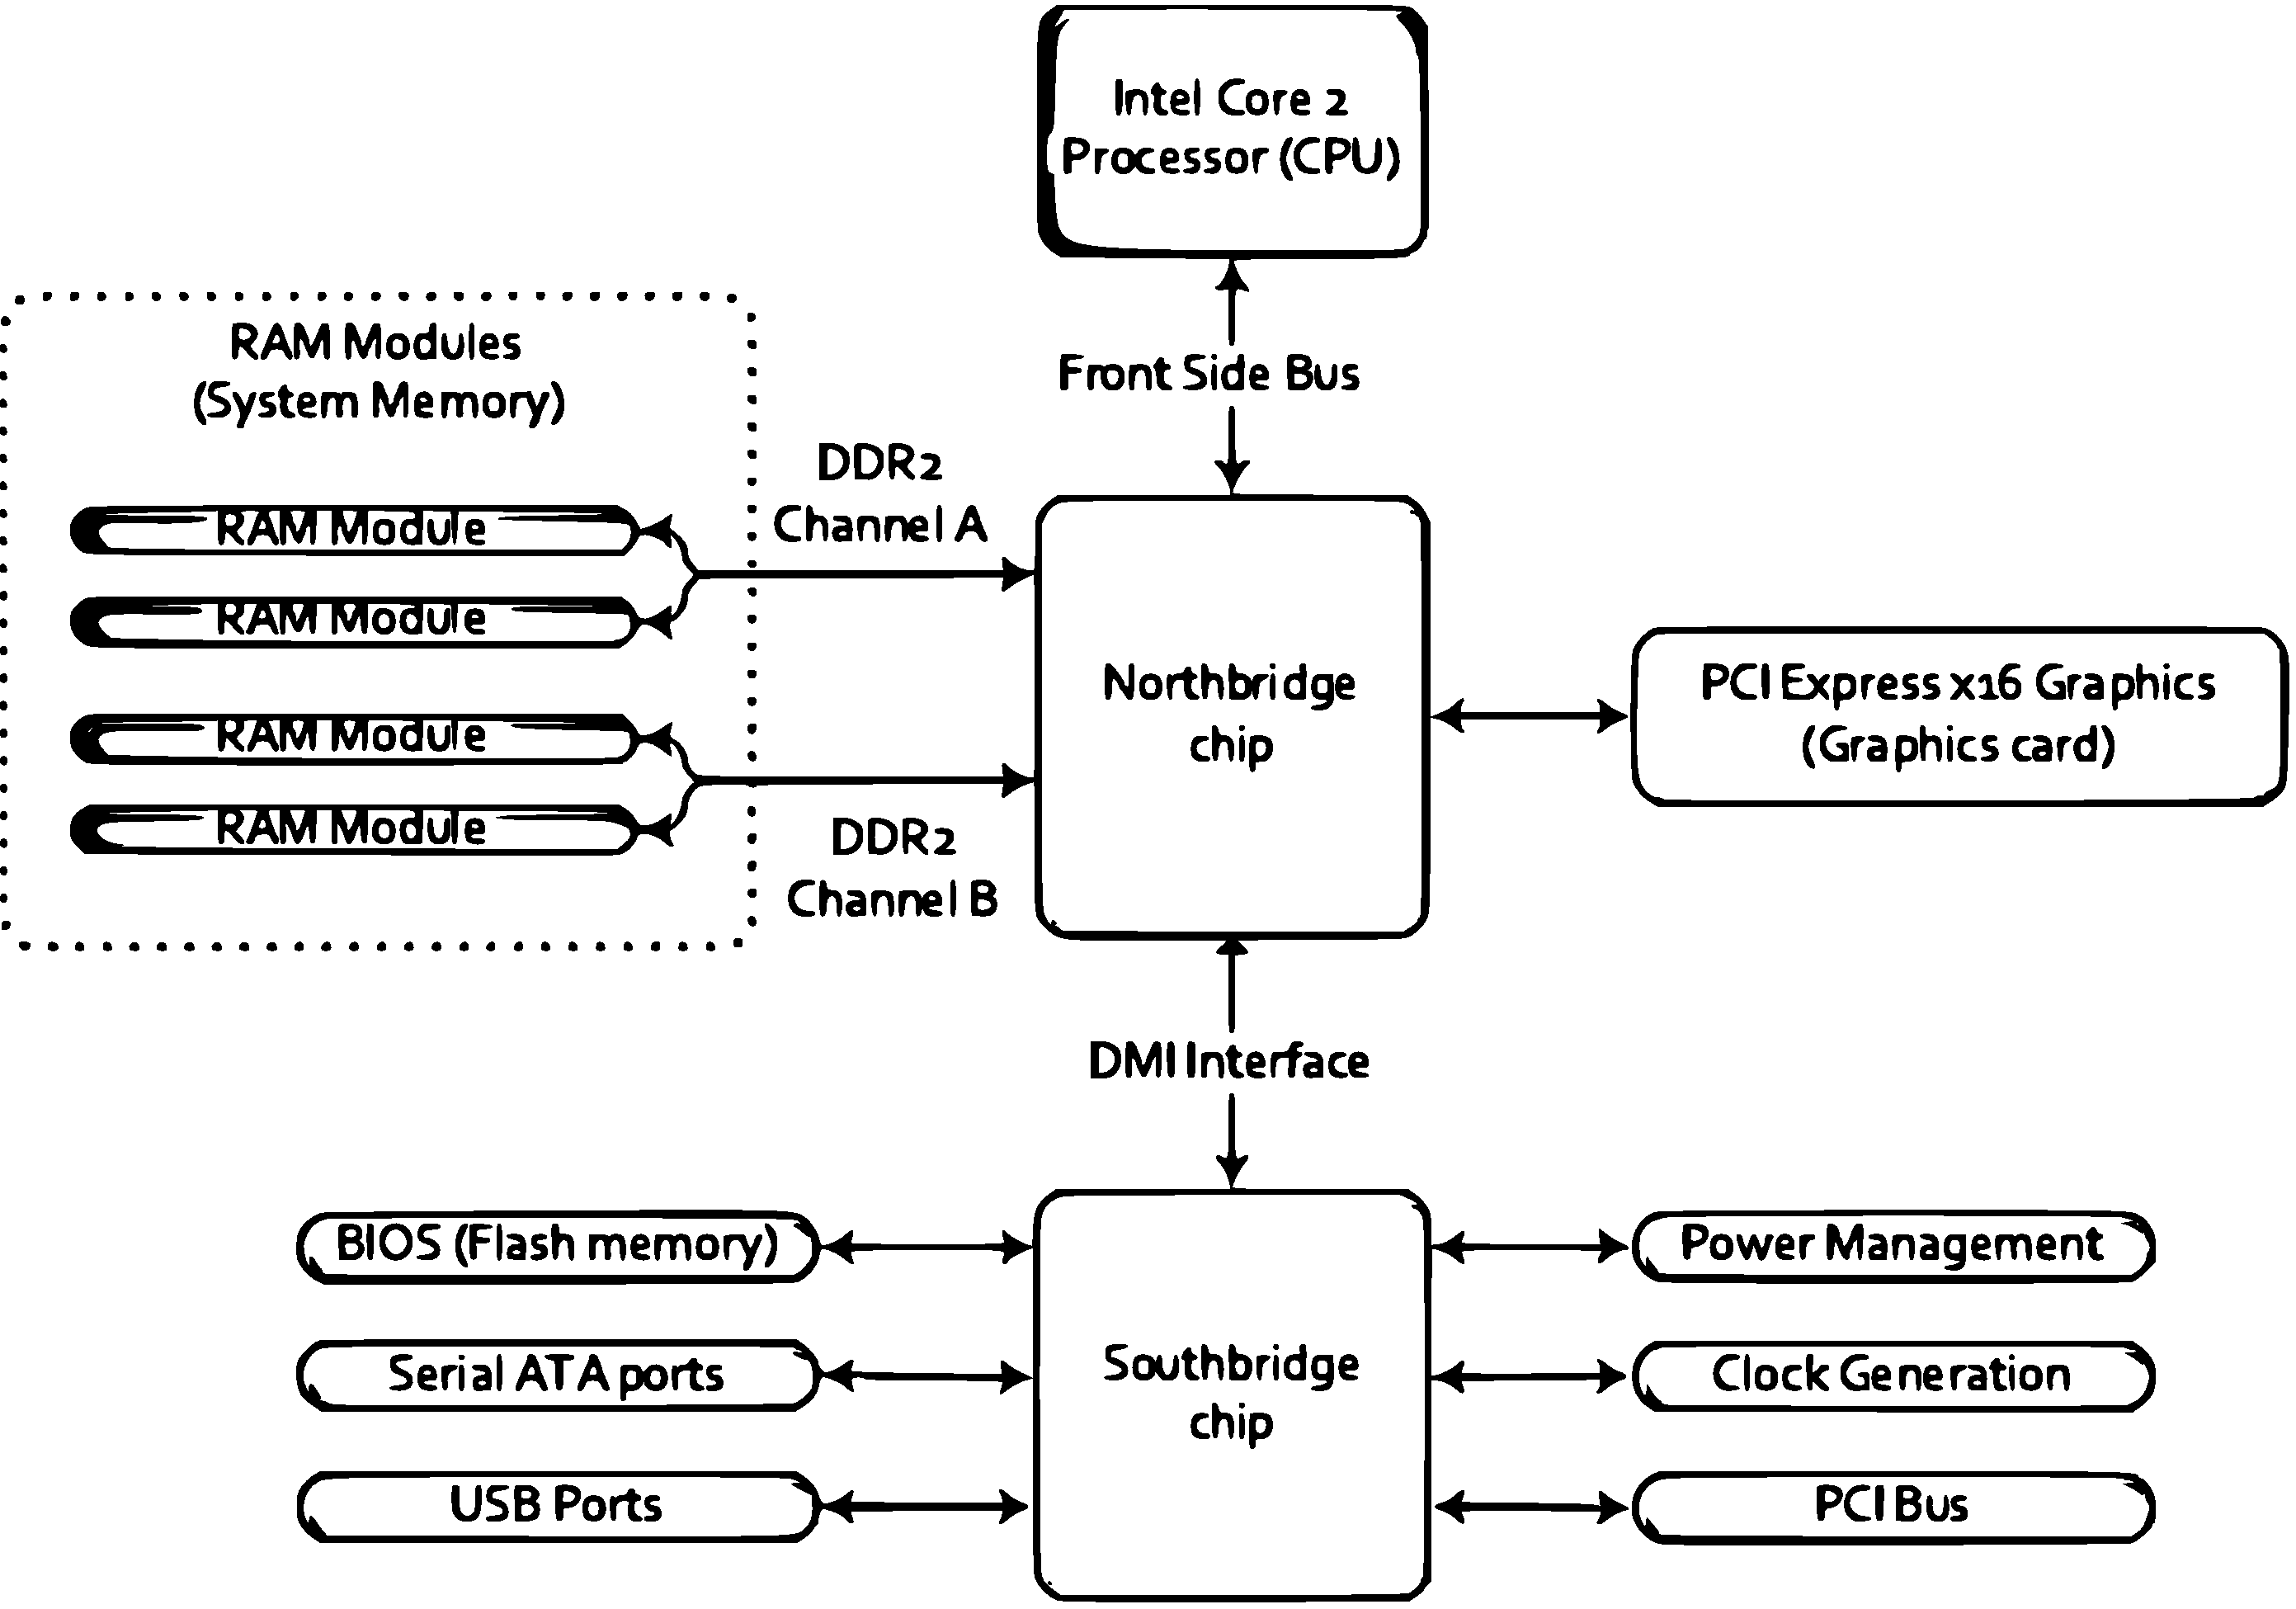
\includegraphics[width=.6\textwidth]{motherboardDiagram}
    }
  \end{center}
\end{frame}

\begin{frame}%{Motherboard Chipsets And The Memory Map}
  \begin{block}{Facts}
    \begin{itemize}
    \item The CPU doesn't know what it's connected to
      \begin{itemize}
      \item[-] CPU test bench?\quad{}network router?\quad{}toaster?\quad{}brain implant?
      \end{itemize}
    \item The CPU talks to the outside world through its pins
      \begin{itemize}
      \item[-] some pins to transmit the physical memory address
      \item[-] other pins to transmit the values
      \end{itemize}
    \item The CPU's gateway to the world is the front-side bus
    \end{itemize}
  \end{block}
  \begin{block}{Intel Core 2 QX6600}
    \begin{itemize}
    \item 33 pins to transmit the physical memory address
      \begin{itemize}
      \item[-] so there are $2^{33}$ choices of memory locations
      \end{itemize}
    \item 64 pins to send or receive data
      \begin{itemize}
      \item[-] so data path is 64-bit wide, or 8-byte chunks
      \end{itemize}
    \end{itemize}
    This allows the CPU to physically address 64GB of memory ($2^{33}\times{}8B$)
  \end{block}
\end{frame}

More info:
\begin{itemize}
\item \href{http://download.intel.com/design/processor/datashts/31559205.pdf}{Datasheet for Intel Core 2 Quad-Core Q6000 Sequence}
\end{itemize}

\begin{frame}%{Motherboard Chipsets And The Memory Map}{ --- Facts}
  \begin{varwidth}{.59\textwidth}
    \textcolor{blue}{Some physical memory addresses are mapped away!}
    \begin{itemize}
    \item only the addresses, not the spaces
    \item Memory holes
      \begin{itemize}
      \item[-] $640KB \sim 1MB$
      \item[-] /proc/iomem
      \end{itemize}
    \item Memory-mapped I/O
      \begin{itemize}
      \item BIOS ROM
      \item video cards
      \item PCI cards
      \item ...
      \end{itemize}
    \end{itemize}
    This is why 32-bit OSes have problems using 4G of RAM.
  \end{varwidth}\hfill
  \begin{varwidth}{.39\textwidth}
    \begin{center}
      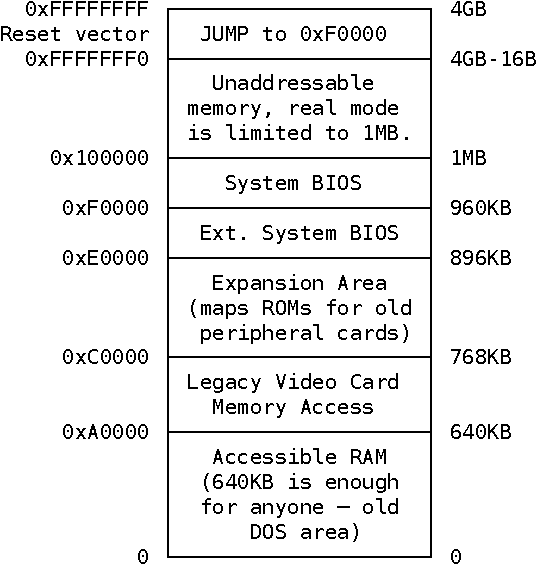
\includegraphics[width=1.2\textwidth]{boot-mem}
    \end{center}
  \end{varwidth}
  \vspace{1em}
  \begin{center}
    What if you don't have 4G RAM?
  \end{center}
\end{frame}

\begin{itemize}
\item \href{http://wiki.osdev.org/Memory_Map_(x86)}{OSDev: Memory Map (x86)}
\end{itemize}

\begin{frame}%{Motherboard Chipsets And The Memory Map}{ --- Facts}
  \begin{block}{the northbridge}
    \begin{enumerate}
    \item receives a physical memory request
    \item decides where to route it
      \begin{itemize}
      \item[-] to RAM? to video card? to ...?
      \item[-] decision made via the \emph{memory address map}
        \begin{itemize}
        \item \code{/proc/iomem}
        \item it is built in \code{setup()}
        \end{itemize}
      \end{itemize}
    \end{enumerate}
  \end{block}
\end{frame}

% \begin{itemize}
% \item When is the memory address map built? \code{setup()}.
% \end{itemize}

\begin{frame}%{Motherboard Chipsets And The Memory Map}{ --- Facts}
  \begin{block}{The CPU modes}
    \begin{description}
    \item[real mode:] CPU can only address 1MB RAM
      \begin{itemize}
      \item 20-bit address, 1-byte data unit
      \end{itemize}
    \item[32-bit protected mode:] can address 4GB RAM
      \begin{itemize}
      \item 32-bit address, 1-byte data unit
      \end{itemize}
    \item[64-bit protected mode:] can address 64GB RAM (Intel Core 2 QX6600)
      \begin{itemize}
      \item 33 address pins, 8-byte data unit
      \end{itemize}
    \end{description}
  \end{block}
  \begin{center}
    \$ \code{grep 'address sizes' /proc/cpuinfo}
  \end{center}
\end{frame}

\begin{itemize}
\item In the comments of
  \href{http://duartes.org/gustavo/blog/post/motherboard-chipsets-memory-map}{Motherboard
    Chipsets and the Memory Map}
  \begin{quote}
    The \emph{physical} stuff is determined by hard-core limits: the actual metal pins
    that stick out of the processor. It is \emph{those} pins that limit the CPU to 64
    gigabytes. That is completely independent of the operating system or even the mode
    (real-mode, 32-bit protected, 64-bit) the CPU is running in. It’s a physical
    limit. That is the limit for which that little multiplication is done. There are 33
    metal pins to transmit an address and 8 metal pins to send and receive data. So
    $2^{33}\times{} 2^3 = 2^{36} = 64 GB$.  The “unit” of transfer in this case is 8
    bytes, that’s the smallest chunk of data the CPU can address on the physical bus. In
    actuality, the CPU usually works in terms of cache lines, which hold 64 bytes in the
    Core 2s. Due to performance, the CPU reads a whole cache line at a time. So if a
    program reads one byte, the CPU actually reads 64 bytes and stores them in the cache.
    The 4-gb limit is logical, not physical. It happens because the registers and
    instructions in the CPU are limited to 32 bits \emph{when it’s running in 32-bit
      mode}, which \emph{does} depend on the OS. Programs need to be able to address
    individual bytes in memory, so the “unit” of addressing is 1 byte. So \emph{that}
    equation becomes $2^{32}\ addresses \times{} 1\ byte\ chunks = 2^{32}\ bytes$, or 4 GB
    total addressing.
  \end{quote}
\end{itemize}

\section{How Computers Boot Up}
\label{sec:how-computers-boot}

See \cite{gustavo2008boot}

\begin{frame}{Bootstrapping}
  \begin{center}
    \mode<beamer>{
      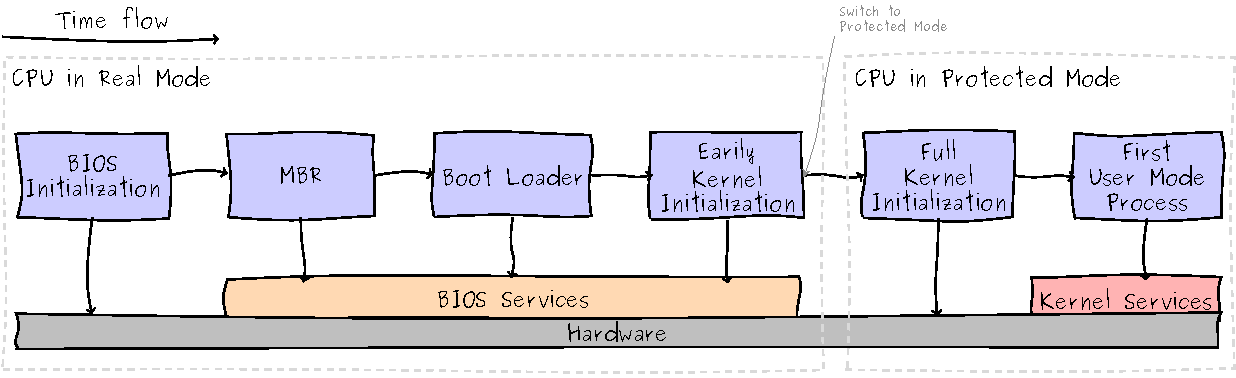
\includegraphics[width=\textwidth]{boot}
    }
    \mode<article>{
      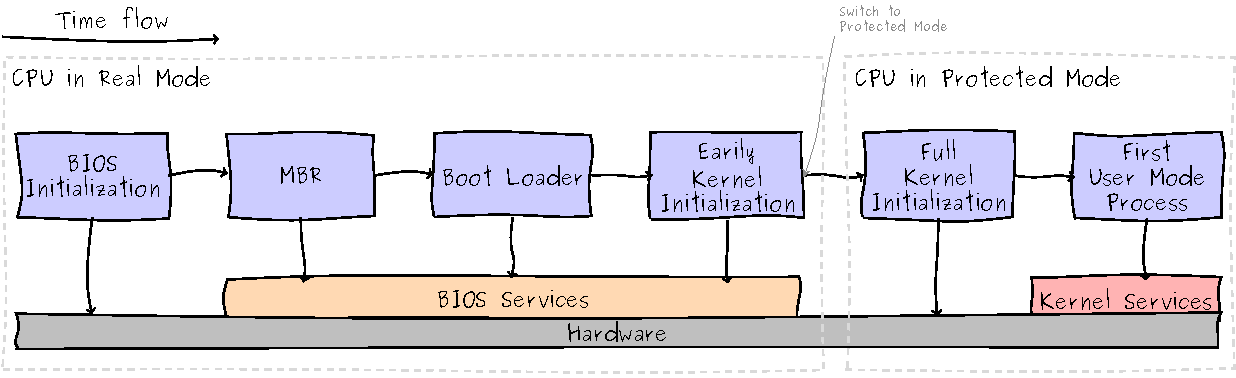
\includegraphics[width=.8\textwidth]{boot}
    }
  \end{center}
  \begin{enumerate}
  \item bringing at least a portion of the OS into main memory, and
  \item having the processor execute it
  \item the initialization of kernel data structures
  \item the creation of some user processes, and
  \item the transfer of control to one of them
  \end{enumerate}
  \begin{center}
    \code{man 7 boot}
  \end{center}
\end{frame}

\subsection{Motherboard power up}
\label{sec:motherboard-power-up}

\begin{frame}
  \begin{block}{Motherboard power up}
    \begin{enumerate}
    \item initializes motherboard firmwares (chipset, etc.)
    \item gets CPU running
    \end{enumerate}
  \end{block}
\end{frame}

\begin{frame}{Real mode}{ --- CPU acts as a 1978 Intel 8086}
  \begin{varwidth}{.52\textwidth}
    \begin{itemize}
    \item any code can write to any place in memory
    \item only 1MB of memory can be addressed
    \item registers are initialized
      \begin{itemize}
      \item[-] \code{EIP} has \code{0xFFFFFFF0}, the \textcolor{blue}{reset vector}
      \item[-] at the reset vector, there is a \code{jump} instruction, jumping to the
        \emph{BIOS entry point} (\code{0xF0000}).%\ (960KB)$, 64KB below 1MB)
      \end{itemize}
    \end{itemize}
  \end{varwidth}\hfill
  \begin{varwidth}{.48\textwidth}
    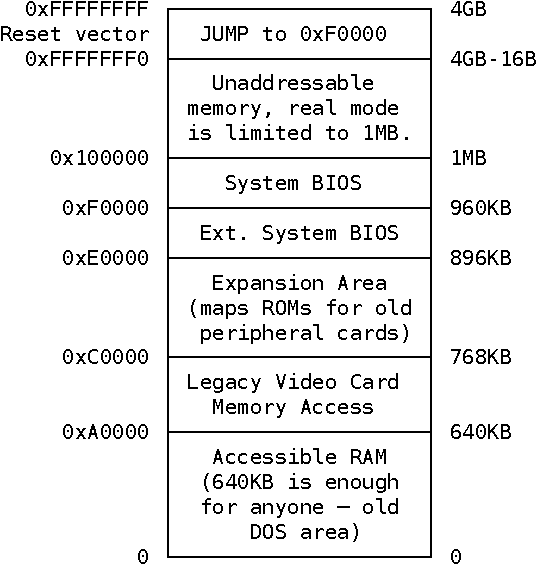
\includegraphics[width=1.15\textwidth]{boot-mem}
  \end{varwidth}
\end{frame}

More info:
\begin{itemize}
\item
  \href{http://stackoverflow.com/questions/7804724/how-is-the-bios-rom-mapped-into-address-space-on-pc}{stackoverflow:
    How is the BIOS rom mapped into address space on PC?}
\item \href{http://www.pcguide.com/ref/mbsys/bios/bootSequence-c.html}{The PC Guide: System
    Boot Sequence}
\item
  \href{http://stackoverflow.com/questions/5300527/do-normal-x86-or-amd-pcs-run-startup-bios-code-directly-from-rom-or-do-they-cop}{stackoverflow:
    Do normal x86 or AMD PCs run startup/BIOS code directly from ROM, or do they copy it
    first to RAM?}
\item \href{http://en.wikipedia.org/wiki/Reset_vector}{Wikipedia: Reset vector}
\item \href{http://lateblt.tripod.com/bit68.txt}{What Happens When A CPU Starts}
\item \href{http://www.freebsd.org/doc/en/books/arch-handbook/boot-bios.html}{FreeBSD:
    BIOS POST}
\item \href{http://www.freebsd.org/doc/en/books/arch-handbook/boot.html}{FreeBSD:
    Bootstrapping and Kernel Initialization}
\end{itemize}

\subsection{BIOS}
\label{sec:bios}

\begin{frame}{BIOS}
  \begin{block}{BIOS uses Real Mode addresses}
    \begin{itemize}
    \item No GDT, LDT, or paging table is needed
      \begin{itemize}
      \item the code that initializes the GDT, LDT, and paging tables must run in Real Mode
      \end{itemize}
    \item Real mode address translation:
      $$\text{segment number}\times{}2^4+offset$$
      \begin{itemize}
      \item[e.g.] to translate \code{<FFFF:0001>} into physical address:
        $$FFFF \times{} 16 + 0001 = FFFF0 + 0001 = FFFF1$$
      \item[if:] \code{offset > 0xF} (overflow)
      \item[then:] \code{address \% $2^{20}$} (wrap around)
      \item only 80286 and later x86 CPUs can address up to:
        $$FFFF0 + FFFF = 10FFEF$$
      \end{itemize}
    \end{itemize}
  \end{block}
\end{frame}

\begin{itemize}
\item \href{http://en.wikipedia.org/wiki/Real_mode}{Wikipedia: Real mode}
\item \href{http://wiki.osdev.org/Real_Mode}{OSDev: Real Mode}
\end{itemize}

\begin{frame}{CPU starts executing BIOS code}
  \begin{enumerate}
  \item POST
    \begin{itemize}
    \item an ACPI-compliant BIOS builds several tables that describe the hardware devices
      present in the system
    \end{itemize}
  \item initializes hardwares
    \begin{itemize}
    \item at the end of this phase, a table of installed PCI devices is displayed
    \end{itemize}
  \item find a boot device
  \item load MBR into \code{0x7c00}
  \item Jump to \code{0x7c00}
  \item MBR moves itself away from \code{0x7c00} (fig~\ref{boot-mem3})
  \end{enumerate}
  \begin{center}
    \mode<beamer>{
      \includegraphics[width=\textwidth]{mbr}
    } \mode<article>{
      \includegraphics[width=.7\textwidth]{mbr}
    }
  \end{center}
\end{frame}

\begin{varwidth}{.65\textwidth}
  \begin{itemize}
  \item The MBR includes a small boot loader, which is loaded into RAM starting from
    address \code{0x00007c00} by the
    BIOS. (\href{http://www.glamenv-septzen.net/en/view/6}{Why \code{0x7c00}}?)
  \item This small program moves itself to the address \code{0x00096a00}, sets up the Real
    Mode stack (ranging from \code{0x00098000} to \code{0x000969ff}), loads the second
    part of the boot loader into RAM starting from address \code{0x00096c00}, and jumps
    into it.
    \begin{description}
    \item[Why move?] because the boot loader may copy the boot sector of a boot partition
      into RAM (\code{0x7c00}) and execute it
    \end{description}
  \end{itemize}
\end{varwidth}\hfill
\begin{varwidth}{.3\textwidth}
  \includegraphics[width=\textwidth]{boot-mem3}
\end{varwidth}

\subsection{The Boot Loader}
\label{sec:boot-loader}

\begin{frame}{GRUB}
  \begin{enumerate}
  \item GRUB stage 1 (in MBR) loads GRUB stage 2
  \item stage 2 reads GRUB configuration file, and presents boot menu
  \item loads the kernel image file into memory (fig~\ref{boot-mem3})
    \begin{itemize}
    \item can't be done in real mode, since it's bigger than 640KB
      \begin{itemize}
      \item BIOS supports \emph{unreal mode}
      \end{itemize}
    \item 1\textsuperscript{st} 512 bytes --- \code{INITSEG, 0x00090000}
    \item \code{setup()} --- \code{SETUPSEG, 0x00090200}
    \item load low --- \code{SYSSEG, 0x00010000}
    \item load high --- \code{0x00100000}
    \end{itemize}
  \item \alert{jumps to the kernel entry point}
    \begin{itemize}
    \item line 80 in \code{2.6.11/arch/i386/boot/setup.S}
      \begin{center}
        \cfbox{red}{\code{jmp trampoline}}
      \end{center}
    \end{itemize}
  \end{enumerate}
\end{frame}

\begin{itemize}
\item \href{http://www.dedoimedo.com/computers/grub.html}{GRUB bootloader - Full tutorial}
\item \code{jmp trampoline} was used in 2.6.11 for calling \code{start\_of\_setup}. In
  newer kernels, a \emph{2-byte jump} is used instead.
  \begin{itemize}
  \item \url{http://lxr.linux.no/linux+v2.6.34/arch/x86/boot/header.S#L112}
  \item \href{http://thestarman.pcministry.com/asm/2bytejumps.htm}{Using SHORT (Two-byte)
      Relative Jump Instructions}
  \item \href{http://www.groad.net/bbs/read.php?tid-3001.html}{2-byte jump in \code{header.S}}
  \end{itemize}
\end{itemize}

\paragraph{More about \emph{unreal mode}:}
\begin{itemize}
\item (\href{http://wiki.osdev.org/Descriptor_Cache}{OSDev: Descriptor cache}) Unreal Mode
  is a 'mode' where the processor runs in real mode while the segment limit does not equal
  64KB (in most cases, its 4GB). Since real mode doesn't update the limit field (of the
  cache), this state persists across segment register loads. Entering this mode is
  achieved easily by entering protected mode (where the limit can be changed), load the
  desired limit into the descriptor cache, then switch back to real mode.
\item (A great post in
  \href{http://forum.osdev.org/viewtopic.php?f=1&t=21179&start=15}{OSDev forum: Unreal
    mode} that deserves a detailed look) The benefits of unreal mode are quite well known:
  access to the 32-bit address space while simultaneously being able to call BIOS and real
  mode programs.
\item \href{http://files.osdev.org/mirrors/geezer/johnfine/segments.htm}{OSDev: Segment
    Registers: Real mode vs. Protected mode} covers \emph{unreal mode}, \emph{NULL
    selector}, \emph{mode switching}
\item \href{http://en.wikipedia.org/wiki/Unreal_mode}{Wikipedia: Unreal mode}
\item \href{http://wiki.osdev.org/Unreal_Mode}{OSDev: Unreal mode}
\end{itemize}

\begin{figure}[h]
  \centering
  \includegraphics[width=.4\textwidth]{nonprogrammable}
  \caption{Descriptor cache register}
  \label{fig:cache-register}
\end{figure}

\paragraph{More about \emph{bootloader}:}
\begin{itemize}
\item \href{http://lennartb.home.xs4all.nl/bootloaders/bootloaders.html}{Linux Boot
    Loaders Compared}
\item \href{http://lennartb.home.xs4all.nl/bootloaders/node3.html}{How Boot Loader Works?}
\end{itemize}
\begin{enumerate}
\item display a "Loading" message
\item load an initial portion of the kernel image from disk:
  \begin{itemize}
  \item the first 512 bytes of the kernel image are put in RAM at address
    \code{0x00090000} (576K, \code{INITSEG})
    \begin{itemize}
    \item \code{hd -n512 /boot/vmlinuz-3.2.0-1-amd64}
    \item \code{/usr/src/linux/arch/i386/boot/bootsect.S}
    \item it was a floppy boot loader, and no longer valid since 2.6
    \item nowadays to make a bootable floppy, you have to use a bootloader as you do with
      a hard disk
    \end{itemize}
  \item the code of the \code{setup()} function (see below) is put in RAM starting
    from address \code{0x00090200} ($576K+512$, \code{SETUPSEG})
  \end{itemize}
\item load the rest of the kernel image from disk and puts the image in RAM starting from
  either low address \code{0x00010000} (64K, \code{SYSSEG}) (for small kernel images ($< 512K$)
  compiled with \code{make zImage}) or high address \code{0x00100000} (1M)(for big kernel
  images ($> 512K$) compiled with \code{make bzImage}).
  \begin{description}
  \item[ISA hole:] Physical addresses ranging from \code{0x000a0000} (640K) to
    \code{0x000fffff} ($1M-1$) are usually reserved to BIOS routines and to map the
    internal memory of ISA graphics cards
  \end{description}
\item Jumps to the \code{setup()} code. (\code{/usr/src/linux/arch/i386/boot/setup.S})
\end{enumerate}
\begin{description}
\item[BIOS interrupt call] \fbox{\code{int \$0x13}} is oftenly seen in
  \code{2.6.11/arch/i386/boot/setup.S}.  \code{INT 13H}, \code{INT 13h}, or \code{INT 19}
  is shorthand for BIOS interrupt call \code{$13_{hex}$}, the 20\textsuperscript{th}
  interrupt vector in an x86-based computer system. The BIOS typically sets up a real mode
  interrupt handler at this vector that provides sector-based hard disk and floppy disk
  read and write services using cylinder-head-sector (CHS) addressing.
\end{description}

\begin{frame}{Memory At Bootup Time}
  \begin{varwidth}{.7\textwidth}
    \begin{block}{The kernel image}
      \begin{itemize}
      \item \code{/boot/vmlinuz-x.x.x-x-x}
      \item has been loaded into memory by the boot loader using the BIOS disk I/O
        services
      \item The image is split into two pieces:
        \begin{itemize}
        \item a small part containing the real-mode kernel code is loaded below the 640K
          barrier
        \item the bulk of the kernel, which runs in protected mode, is loaded after the
          first megabyte of memory
        \end{itemize}
      \end{itemize}
    \end{block}
  \end{varwidth}\hfill
  \begin{varwidth}{.25\textwidth}\label{boot-mem3}
    \includegraphics[width=1.3\textwidth]{boot-mem3}
  \end{varwidth}
\end{frame}

\begin{itemize}
\item More info about boot-time memory arrangement, see \cite{linux2.6.25protocol}.
\end{itemize}

\section{The Kernel Boot process}
\label{sec:kernel-boot-process}

% \subsection{The Linux/i386 boot protocol}

% \begin{frame}{The Linux Kernel Uses A Rather Complicated Boot Convention}
%   Due to:
%   \begin{itemize}
%   \item historical aspects
%   \item in the early days to have the kernel itself be a bootable image
%   \item the complicated PC memory model
%   \item real-mode DOS as a mainstream operating system
%   \end{itemize}
% \end{frame}

% \subsection{RAM contents after boot loader is done}

% % \begin{frame}{RAM contents after boot loader is done}
% %   \begin{center}
% %     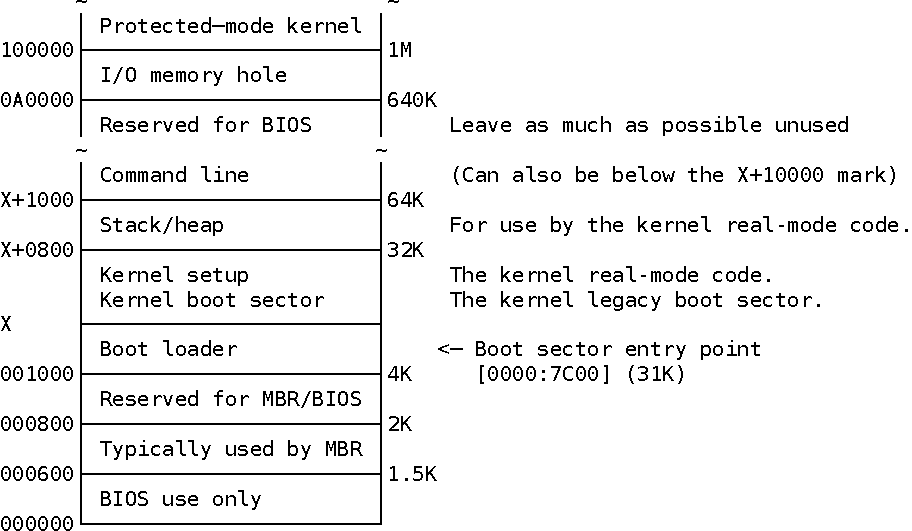
\includegraphics[width=\textwidth]{boot-mem2}
% %   \end{center}
% %   \scriptsize{where the address X is as low as the design of the boot loader permits}
% % \end{frame}

% \begin{frame}{RAM contents after boot loader is done}
%   \mode<beamer>{
%     \begin{center}
%       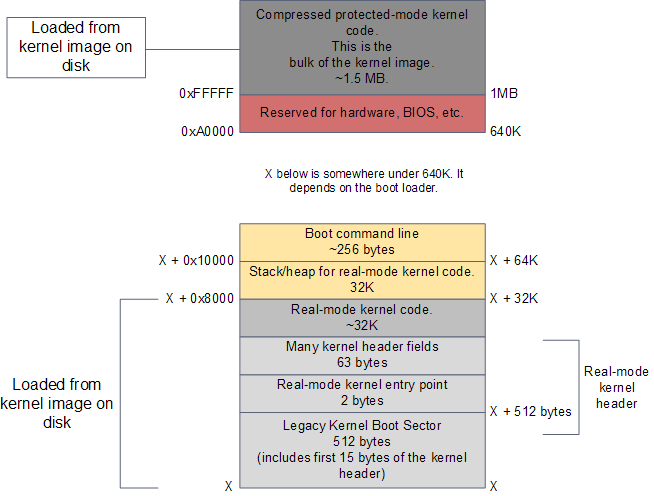
\includegraphics[width=.9\textwidth]{memoryAfterBootloader}
%     \end{center}
%   }
%   \mode<article>{
%     \begin{center}
%       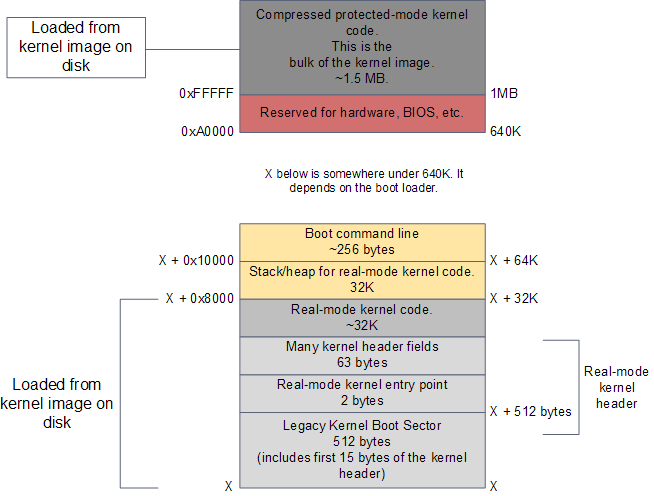
\includegraphics[width=.8\textwidth]{memoryAfterBootloader}
%     \end{center}
%   }
% \end{frame}

% \begin{itemize}
% \item Picture source: \cite{gustavo2008proess}, \cite{gustavo2008boot}
%   \begin{itemize}
%   \item This memory map is for 2.6.25, and not fully compatible with 2.6.11.
%   \end{itemize}
% \item More info about boot-time memory arrangement, see \cite{linux2.6.25protocol}.
% \end{itemize}

\subsection{setup()}

\begin{frame}{The \code{setup()} Function}
  boots and loads the executable image to ($0x9000\ll 4$) and jumps to ($0x9020\ll 4$)
  \begin{center}
    \mode<beamer>{
      
\includegraphics[width=\textwidth]{setup2}
    } \mode<article>{
      
\includegraphics[width=.7\textwidth]{setup2}
    }
  \end{center}
  \begin{itemize}
  \item \code{2.6.11/arch/i386/boot/setup.S}
  \item Re-initialize all the hardware devices
  \item Sets the A20 pin (turn off \emph{wrapping around})
  \item Sets up a provisional IDT and a provisional GDT %(line 792 in \code{setup.S})
    % \item the uncompressed part of the Linux kernel decompresses the compressed portion
    %   to
    %   address ($0x10000\ll 4$) (1M) and kernel initialization begins
  \item \code{PE=1, PG=0} in \code{cr0} %(line 824 in \code{setup.S})
  \item jump to \code{startup\_32()}
  \end{itemize}
\end{frame}

\begin{itemize}
\item \emph{Kernel attributes} are stored at the end of the boot block
  (1\textsuperscript{st}
  sector). (\href{http://lxr.linux.no/linux+v2.6.11/arch/i386/boot/bootsect.S#L90}{line 90 in
    \code{bootsect.S}})
\item
  \href{http://lists.kernelnewbies.org/pipermail/kernelnewbies/2011-March/001133.html}{From
    which point onwards the kernel execution starts?}
\item
  \href{http://unixbhaskar.blogspot.com/2010/03/insight-into-gnulinux-boot-process.html}{Insight
    into GNU/Linux boot process}
\item
  \href{http://linux-development-for-fresher.blogspot.com/2012/07/linux-boot-process-in-nutshell.html}{Linux
    Boot Process in a nutshell}
\item The \code{setup()} function:
  \begin{enumerate}
  \item Builds system's physical memory map
    \begin{itemize}
    \item find the amount of memory present in the system (sec 1.1 in
      \cite{abhishek2002memory}, \href{http://lxr.linux.no/linux-old+v2.4.19/arch/i386/boot/setup.S#L289}{\code{arch/i386/boot/setup.S}
        (2.4.19)}, line 289-389)
    \end{itemize}
  \item Sets the keyboard repeat delay and rate
  \item Initializes the video adapter card
  \item Reinitializes the disk controller and determines the hard disk parameters
  \item Checks for an IBM Micro Channel bus (MCA)
  \item Checks for a PS/2 pointing device (bus mouse)
  \item Checks for Advanced Power Management (APM ) BIOS support
  \item If the BIOS supports the Enhanced Disk Drive Services (EDD ), builds a table in
    RAM describing the hard disks available in the system
  \item If the kernel image was loaded low in RAM (at physical address 0x00010000), the
    function moves it to physical address \texttt{0x00001000} (was used by boot loader).
    \begin{description}
    \item[Why?] (Sec A.3, \emph{Middle Ages: the \code{setup()} Function},
      \cite{bovet2005understanding}) This step is necessary because to be able to store
      the kernel image on a floppy disk and to reduce the booting time, the kernel image
      stored on disk is compressed, and the decompression routine needs some free space to
      use as a temporary buffer following the kernel image in RAM.
      \begin{itemize}
      \item \code{BOOTSEG = 0x07C0}. This is 27K above \code{0x1000}. It was too small to
        hold the kernel image. After boot loader is done, \code{BOOTSEG (0x7C00)} is
        free. So kernel image can be stuffed here.
      \end{itemize}
    \item[Memory layout]
      (\href{http://unixbhaskar.blogspot.com/2010/03/insight-into-gnulinux-boot-process.html}{Insight into GNU/Linux Boot Process})

      \textbf{uncompressed image:} ... Later, all the kernel is moved from \code{0×10000}
      (64K) to \code{0×1000} (4K). This move overwrites BIOS data stored in RAM, so BIOS
      calls can no longer be performed. We don’t care because linux dosen’t use BIOS to
      acces the hardware. The first physical page is not touched because it is the
      so-called “zero-page”, used in handling virtual memory.  At this point,
      \code{setup.S} enters protected mode and jumps to \code{0×1000}, where the kernel
      lives. All the available memory can be accessed now, and the system can begin to
      run.

      The steps just described were once the whole story of booting when the kernel was
      small enough to fit in half a megabyte of memory --- the address range between
      \code{0×10000} and \code{0×90000}. As features were added to the system, the kernel
      became larger than half a megabyte and could no longer be moved to
      \code{0×1000}. Thus, code at \code{0×1000} is no longer the Linux kernel, instead
      the “gunzip” part of the gzip program resides at that address.

      \textbf{Compressed image [zimage]:} When the kernel is moved to \code{0×1000} (4K),
      \code{head.S} in the compressed directory is sitting at this address. It's in charge
      of gunzipping the kernel, this done by a function \code{decompress\_kernel()},
      defined in \code{compressed/misc.c}, which in turns calls \code{inflate()} which
      writes its output starting at address \code{0×100000} (1MB). High memory can now be
      accessed, because \code{setup.S} han take us to the protected mode now.  After
      decompression, \code{head.S} jumps to the actual beginning of the kernel. The
      relevant code is in \code{../kernel/head.S}. \code{head.S} (i.e., the code found at
      \code{0×100000}) can complete processor initialization and call
      \code{start\_kernel()}.

      The boot steps shown above rely on the assumption that the compressed kernel can fit
      in half a megabyte of space. While this is true most of the time, a system stuffed
      with device drivers might not fit into this space. For example, kernels used in
      installation disks can easily outgrow the available space. To solve this problem
      problem bzImage kernel images were introduced.

      \textbf{Big Compressed Image [bzImage]:} This kind of kernel image boots similarly
      to zImage, with a few changes.

      When the system is loaded at \code{0×10000} (64K) a special helper routine is called
      which does some special BIOS calls to move the kernel to \code{0×100000}
      (1Mb). \code{setup.S} doesn’t move the system back to \code{0×1000} (4K) but, after
      entering protected mode, jumps instead directly to address \code{0×100000} (1MB) where data
      has been moved by the BIOS in the previous step.  The decompresser found at 1MB
      writes the uncompressed kernel image into low memory until it is exhausted, and then
      into high memory after the compressed image.  The two pieces are then reassembled to
      the address \code{0×100000} (1MB). Several memory moves are needed to perform the task
      the address \code{0×100000} (1MB). Several memory moves are needed to perform the task
      correctly.
    \end{description}
    
    \begin{gascode}
      code32_start:               # here loaders can put a different
                                  # start address for 32-bit code.
      #ifndef __BIG_KERNEL__
              .long     0x1000    #   0x1000 = default for zImage
      #else
              .long     0x100000  # 0x100000 = default for big kernel
      #endif
    \end{gascode}
    \clearpage
    The default value of \code{code32} is \code{\_\_BOOT\_CS:0x1000} (\code{\_\_BOOT\_CS}
    = 16). (\href{http://lxr.linux.no/linux+v2.6.11/arch/i386/boot/setup.S#L855}{Line
      855-857})
    
    \begin{gascode}
      code32: .long 0x1000    # will be set to 0x100000 for big kernels
      .word __BOOT_CS
    \end{gascode}

    It will be changed to
    \code{\_\_BOOT\_CS:0x100000}. (\href{http://lxr.linux.no/linux+v2.6.11/arch/i386/boot/setup.S#L594}{Line
      594-595})
    
    \begin{gascode}
      movl %cs:code32_start, %eax
      movl %eax, %cs:code32
    \end{gascode}
    \code{\%cs:code32\_start} $\Rightarrow$ \code{\%cs:code32} = \code{0x10:0x100000} (for
    load high, i.e. bzImage)
\item Sets the \href{http://en.wikipedia.org/wiki/A20_line}{\code{A20}} pin located on
    the 8042 keyboard controller (for switching to pmode)
  \item Sets up a provisional
    \href{http://en.wikipedia.org/wiki/Interrupt_descriptor_table}{Interrupt Descriptor
      Table (IDT)} and a provisional
    \href{http://en.wikipedia.org/wiki/Global_Descriptor_Table}{Global Descriptor Table
      (GDT)}.
    \begin{itemize}
    \item \href{http://lxr.linux.no/linux+v2.6.11/arch/i386/boot/setup.S#L792}{line 792 in
        \code{setup.S}}
    \item \href{http://lxr.linux.no/linux+v2.6.11/include/asm-i386/segment.h#L83}{line 83-89 in \code{include/asm-i386/segment.h}}
    \end{itemize}
    The provisional GDT is created with 2 useful entries, each covering the whole 4GB
    address space \cite{abhishek2002memory}. The code that loads the GDT is:
    \begin{gascode}
      xorl %eax, %eax # Compute gdt_base
      movw %ds, %ax   # (Convert %ds:gdt to a linear ptr)
      shll $4, %eax
      addl $gdt, %eax
      movl %eax, (gdt_48+2)
      lgdt gdt_48     # load gdt with whatever is appropriate
    \end{gascode}
\begin{itemize}
\item \code{\%ds = \%cs = SETUPSEG = 0x9020}
\item \code{\$gdt} --- beginning address of the GDT table (somewhere offsetting in
  \code{\%ds}). Its actual value will be determined at assemble time by the assembler (p24
  in \cite{bartlett2009programming})
\item \code{gdt\_48}: a label in \code{setup.S}
  (\href{http://lxr.linux.no/linux+v2.6.11/arch/i386/boot/setup.S#L1006}{line
    1006}). \code{gdt\_48+2} will be filled with the \emph{gdt base} computed above.
\item \code{lgdt}: loads the value in \code{gdt\_48} into \code{GDTR}
\item \code{gdt\_48 = limit,base} $\Rightarrow$ \code{GDTR}
  \begin{itemize}
  \item \code{limit = gdt\_end - gdt - 1 = 31} (16 bits)
  \item \code{base = \%ds $\ll$ 4 + gdt} (32 bits)
  \end{itemize}
\end{itemize}
\begin{gascode}
gdt_48:
     .word      gdt_end - gdt - 1   # gdt limit
     .word      0, 0                # gdt base (filled in later)

gdt:
     .fill GDT_ENTRY_BOOT_CS,8,0

     .word      0xFFFF   # 4Gb - (0x100000*0x1000 = 4Gb)
     .word      0        # base address = 0
     .word      0x9A00   # code read/exec
     .word      0x00CF   # granularity = 4096, 386
                         #  (+5th nibble of limit)

     .word      0xFFFF   # 4Gb - (0x100000*0x1000 = 4Gb)
     .word      0        # base address = 0
     .word      0x9200   # data read/write
     .word      0x00CF   # granularity = 4096, 386
                         #  (+5th nibble of limit)
gdt_end:
\end{gascode}
\begin{itemize}
\item \code{gdt}: the provisional GDT has 4 entries.
  \begin{itemize}
  \item The 1\textsuperscript{st} and 2\textsuperscript{nd} entries are initialized to
    0\footnote{\code{.fill REPEAT,SIZE,VALUE}}
    (\href{http://lxr.linux.no/linux+v2.6.11/arch/i386/boot/setup.S#L983}{line 983}), as
    required by Intel.
    \begin{center}
      \code{.fill GDT\_ENTRY\_BOOT\_CS,8,0}
    \end{center}
  \item 3\textsuperscript{rd} is \code{\_\_BOOT\_CS}
  \item 4\textsuperscript{th} is \code{\_\_BOOT\_DS}
  \end{itemize}
  (\href{http://www.tldp.org/HOWTO/Linux-Init-HOWTO-3.html}{Linux HOWTO: Prepare to move
    to protected mode}) Calculate the linear base address of the kernel GDT (table) and
  load the GDT pointer register with its base address and limit.
  \begin{figure}[h]
    \centering
    \includegraphics[width=.3\textwidth]{gdt-boot}
    \caption{Provisional GDT in RAM}
    \label{fig:gdt-boot}
  \end{figure}
  \begin{itemize}
  \item This early kernel GDT describes kernel code as 4 GB, with base address 0,
    code/readable/executable, with granularity of 4 KB.
    \begin{figure}[h]
      \centering
      \includegraphics[width=.6\textwidth]{gdt-entry-cs}
      \caption{Code segment descriptor value: \texttt{0x00CF9A000000FFFF}}
      \label{fig:cs}
    \end{figure}
  \item The kernel data segment is described as 4 GB, with base address 0,
    data/readable/writable, with granularity of 4 KB.
    \begin{figure}[h]
      \centering
      \includegraphics[width=.6\textwidth]{gdt-entry-ds}
      \caption{Data segment descriptor value: \texttt{0x00CF92000000FFFF}}
      \label{fig:ds}
    \end{figure}
  \end{itemize}
\end{itemize}
  \item Resets the floating-point unit (FPU), if any.
  \item Reprograms the Programmable Interrupt Controllers (PIC) to mask all interrupts,
    except IRQ2 which is the cascading interrupt between the two PICs.
  \item Switches the CPU from Real Mode to Protected Mode by setting the \code{PE} bit in
    the \code{cr0} status register. The \code{PG} bit in the \code{cr0} register is
    cleared, so paging is still
    disabled. (\href{http://lxr.linux.no/linux+v2.6.11/arch/i386/boot/setup.S#L832}{line
      832-833})
\begin{gascode}
  movw $1, %ax # protected mode (PE) bit
  lmsw %ax     # This is it!
\end{gascode}
    \begin{itemize}
    \item \code{lmsw} --- \href{http://www.fermi.mn.it/linux/quarta/x86/lmsw.htmlink}{Load
        Machine Status Word} (part of \code{cr0})
    \item in later kernel (e.g. 2.6.34) the switching code is like this (\href{http://lxr.linux.no/linux+v2.6.34/arch/x86/boot/pmjump.S#L39}{line 39-41 in pmjump.S}):
\begin{gascode}
  movl %cr0, %edx
  orb $X86_CR0_PE, %dl # Protected mode
  movl %edx, %cr0
\end{gascode}
      \href{http://lxr.linux.no/linux+v2.6.34/arch/x86/include/asm/processor-flags.h#L29}{line
      29 in \code{processor-flags.h}}:
    \begin{center}
      \code{\#define X86\_CR0\_PE 0x00000001}
    \end{center}
  \end{itemize}
  \textbf{NOTE:} We are now in 32-bit protected mode. From now on, the address translation will be
  done by looking up the GDT table.
  \item Jumps to the \code{startup\_32()} assembly language function. (\href{http://lxr.linux.no/linux+v2.6.11/arch/i386/boot/setup.S#L854}{line 854})
    \begin{gascode}
        .byte 0x66, 0xea   # prefix + jmpi-opcode
code32: .long   0x1000     # will be set to 0x100000
                           # for big kernels
        .word   __BOOT_CS
      \end{gascode}
\begin{itemize}
\item \code{jmpi 0x100000,\_\_BOOT\_CS} (far jump)
  \begin{itemize}
  \item jump to \code{0x10:0x100000} (segment number: \code{0x10}; offset: \code{0x100000}.)
  \end{itemize}
\item
  (\href{http://unixbhaskar.blogspot.com/2010/03/insight-into-gnulinux-boot-process.html}{Insight
    into GNU/Linux boot process}) At the end of the initial assembly code in
  \code{arch/i386/boot/setup.S} a jump to offset \code{0x100000} in segment
  \code{KERNEL\_CS} is called. This is where the version of \code{startup\_32()} found in
  \code{arch/i386/boot/compress-ed/head.S}. But the jump is a little tricky, as we haven’t
  yet reloaded the \code{CS} register, the default size of the target offset still is 16
  bit. However, using an operand prefix (\code{0×66}), the CPU will properly take our 48
  bit far pointer [\code{.byte 0x66, 0xea}].
\end{itemize}
  \end{enumerate}
\end{itemize}


% \begin{frame}{The real-mode kernel header}
%   The action starts in \emph{the real-mode kernel header}
%   \begin{itemize}
%   \item This region of memory is used to implement the Linux boot protocol between the
%     boot loader and the kernel
%   \item \emph{Documentation/i386/boot.txt}
%   \end{itemize}
% \end{frame}

% \begin{frame}{The real-mode kernel header}
%   \begin{block}{\emph{arch/i386/boot/bootsect.S}}
%     \begin{center}
%       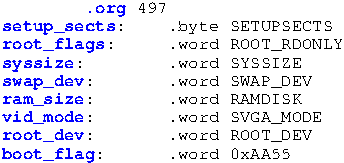
\includegraphics[width=.7\textwidth]{kernel-header}
%     \end{center}
%   \end{block}
%   \cfbox{red}{hd -n512 /boot/vmlinuz-x.x.x-x-x}
% \end{frame}

\subsection{startup\_32()}

\begin{frame}{\code{setup() -> startup\_32()}}%{The real mode entry point}
  \begin{block}{\code{startup\_32()} for compressed kernel}
    \begin{itemize}
    \item in \code{arch/i386/boot/compressed/head.S}
      \begin{itemize}
      \item physically at
        \begin{itemize}
        \item[]\code{0x00100000} --- load high, or
        \item[]\code{0x00001000} --- load low
        \end{itemize}
      \item does some basic register initialization
      \item \code{decompress\_kernel()}
      \end{itemize}
    \item the uncompressed kernel image has overwritten the compressed one starting at 1MB
    \item jump to the protected-mode kernel entry point at 1MB of RAM ($0×10000\ll 4$)
      \begin{itemize}
      \item \code{startup\_32()} for real kernel
      \end{itemize}
    \end{itemize}
  \end{block}
\end{frame}

\begin{itemize}
\item Initializing registers
  (\href{http://lxr.linux.no/linux+v2.6.11/arch/i386/boot/compressed/head.S#L31}{line 31
    in \code{head.S}})

  \begin{varwidth}{.3\textwidth}
    \begin{gascode}
startup_32:
        cld
        cli
        movl $(__BOOT_DS),%eax
        movl %eax,%ds
        movl %eax,%es
        movl %eax,%fs
        movl %eax,%gs

        lss stack_start,%esp
    \end{gascode}
  \end{varwidth}
    \begin{itemize}
  \item \code{cld}: clear direction flag
  \item \code{cli}: clear interrupt flag
  \item \code{lss stack\_start,\%esp}: load \code{\%ss} and \code{\%esp} pair
    (\code{\%ss:\%esp}) in a single instruction using the value stored in
    \code{stack\_start}.
    (\href{http://lxr.linux.no/linux+v2.6.11/arch/i386/boot/compressed/head.S#L40}{line 40
      in \code{head.S}})
    \begin{itemize}
    \item \code{lss} --- read a full pointer from memory and store it in the selected
      segment register:register pair. (p332, \cite{intel86})
    \end{itemize}
    % load values stored in \code{stack\_start} into \code{ss:esp}
  \item \code{stack\_start}
    (\href{http://lxr.linux.no/linux+v2.6.11/arch/i386/boot/compressed/misc.c#L296}{line
      296-303 in \code{misc.c}})

    \begin{ccode}
      struct {
        long * a;
        short b;
      } stack_start = { & user_stack [STACK_SIZE] , __BOOT_DS };
    \end{ccode}
  \item \code{STACK\_SIZE} = 4096
  \item \code{\_\_BOOT\_DS} = 24 (segment selector) $\Rightarrow$ \code{\%ss}
    \begin{itemize}
    \item the 4\textsuperscript{th} (2\textsuperscript{nd} non-zero) entry in provisional
      GDT (sec 1.2 in \cite{abhishek2002memory}). Each entry is 8 bytes.
    \end{itemize}
  \item \code{\&user\_stack[4096]} $\Rightarrow$ \code{\%esp}
  \end{itemize}
\item Clear BSS (line 55 in
  \href{http://lxr.linux.no/linux+v2.6.11/arch/i386/boot/compressed/head.S#L55}{head.S})

  \begin{varwidth}{.2\textwidth}
    \begin{gascode}
xorl %eax,%eax
movl $_edata,%edi
movl $_end,%ecx
subl %edi,%ecx
cld
rep
stosb
    \end{gascode}
  \end{varwidth}
  \begin{itemize}
  \item \href{http://www.cs.ubbcluj.ro/~dadi/ac/doc/ng1d5fc.html}{\code{stosb}} copies the
    value in \code{AL} into the location pointed to by \code{ES:DI}. \code{DI} is then
    incremented (if the direction flag is cleared) or decremented (if the direction flag
    is set), in preparation for storing \code{AL} in the next location.
  \item \code{rep} --- repeat
  \item
    (\href{http://stackoverflow.com/questions/3818856/what-does-this-assembly-do}{Stackoverflow:
      What does \code{rep stos} do?}) For \code{ecx} repetitions, stores the contents of
    \code{eax} into where \code{edi} points to, incrementing or decrementing \code{edi}
    (depending on the direction flag) by 4 bytes each time. Normally, this is used for a
    memset-type operation.

    Usually, that instruction is simply written \code{rep stosd}. Experienced assembly
    coders know all the details mentioned above just by seeing that. :-)

    ETA for completeness (thanks PhiS): Each iteration, \code{ecx} is decremented by 1,
    and the loop stops when it reaches zero. For \code{stos}, the only thing you will
    observe is that \code{ecx} is cleared at the end.
  \end{itemize}
\end{itemize}

\begin{frame}{\code{startup\_32()} for real kernel}
  \begin{block}{\code{startup\_32()} in \code{arch/i386/kernel/head.S}}
    \begin{itemize}
    \item Zeroes the kernel BSS for protected mode
    \item sets up the final GDT
    \item builds provisional kernel page tables so that paging can be turned on
    \item enables paging (\code{cr3->PGDir; PG=1} in \code{cr0})
    \item initializes a stack
    \item \code{setup\_idt()} --- creates the final interrupt descriptor table
    \item \code{gdtr->GDT; idtr->IDT}
    \item \code{start\_kernel()}
    \end{itemize}
  \end{block}
\end{frame}

\begin{itemize}
\item Sets up the final GDT
  (line \href{http://lxr.linux.no/linux+v2.6.11/arch/i386/kernel/head.S#L63}{63},
  \href{http://lxr.linux.no/linux+v2.6.11/arch/i386/kernel/head.S#L303}{303},
  \href{http://lxr.linux.no/linux+v2.6.11/arch/i386/kernel/head.S#L448}{448-450},
  \href{http://lxr.linux.no/linux+v2.6.11/arch/i386/kernel/head.S#L459}{459-463},
  \href{http://lxr.linux.no/linux+v2.6.11/arch/i386/kernel/head.S#L470}{470-EOF} in \code{head.S})
    \begin{gascode}
        lgdt boot_gdt_descr - __PAGE_OFFSET

        ...
        lgdt cpu_gdt_descr
        ...
        
boot_gdt_descr:
        .word __BOOT_DS+7                     # limit (31, end of DS)
        .long boot_gdt_table - __PAGE_OFFSET  # base location

ENTRY(boot_gdt_table)
        .fill GDT_ENTRY_BOOT_CS,8,0
        .quad 0x00cf9a000000ffff    # kernel 4GB code at 0x00000000 
        .quad 0x00cf92000000ffff    # kernel 4GB data at 0x00000000 

cpu_gdt_descr:
        .word GDT_ENTRIES*8-1
        .long cpu_gdt_table

        .fill NR_CPUS-1,8,0             # space for the other GDT descriptors
        
ENTRY(cpu_gdt_table)
        ...
        # Entry 12-15 
        .quad 0x00cf9a000000ffff    # 0x60 kernel 4GB code at 0x00000000 
        .quad 0x00cf92000000ffff    # 0x68 kernel 4GB data at 0x00000000 
        .quad 0x00cffa000000ffff    # 0x73 user 4GB code at 0x00000000 
        .quad 0x00cff2000000ffff    # 0x7b user 4GB data at 0x00000000 
        ...
      \end{gascode}
    \begin{itemize}
    \item \code{.fill REPEAT, SIZE, VALUE}
      \begin{itemize}
      \item \code{.fill 2,8,0} fills the 1\textsuperscript{st} and 2\textsuperscript{nd}
        entry with \code{0}
      \end{itemize}
    \item \code{.quad} 8-byte datas (the 3\textsuperscript{rd} and 4\textsuperscript{th}
      entry)
    \item The addresses of \code{boot\_gdt\_table} and \code{cpu\_gdt\_table} will be
      assigned by assembler at compile time.
    \end{itemize}
  \item Zeroes the kernel BSS (line 74-79 in \code{arch/i386/kernel/head.S})
      \begin{gascode}
        xorl %eax,%eax
        movl $__bss_start - __PAGE_OFFSET,%edi
        movl $__bss_stop - __PAGE_OFFSET,%ecx
        subl %edi,%ecx
        shrl $2,%ecx
        rep ; stosl
      \end{gascode}
    \begin{itemize}
    \item \code{subl \%edi, \%ecx} --- get BSS size, put into \code{\%ecx}
    \item \code{shrl \$2,\%ecx} --- \code{$\frac{\%ecx}{4}$}, get number of 4-byte chunks
      (repeat times)
    \item
      \href{http://pdos.csail.mit.edu/6.828/2004/readings/i386/STOS.htm}{\code{stosl}/\code{stosd}}
      --- Store \code{EAX} in dword \code{ES:EDI}, update \code{EDI}
    \end{itemize}
\item Initialize page tables (Sec 2.5.5, \emph{Kernel Page Tables}, \cite{bovet2005understanding})
  \begin{itemize}
  \item In the first phase, the kernel creates a limited address space including the
    kernel's code and data segments, the initial Page Tables, and 128 KB for some dynamic
    data structures. This minimal address space is just large enough to install the kernel
    in RAM and to initialize its core data structures.
  \item The provisional Page Global Directory is contained in the \code{swapper\_pg\_dir}
    variable. \code{swapper\_pg\_dir} is at the beginning of BSS (uninitialized data area)
    because BSS is no longer used after system start up.
  \item The provisional Page Tables are stored starting from \code{pg0}, right after the
    end of the kernel's uninitialized data segments (\code{\_end}).
  \item For the sake of simplicity, let's assume that the kernel's segments, the
    provisional Page Tables, and the 128 KB memory area fit in the first 8 MB of RAM. In
    order to map 8 MB of RAM, two Page Tables are required.
  \item The objective of this first phase of paging is to allow these 8 MB of RAM to be
    easily addressed both in real mode and protected mode.
    \begin{center}
      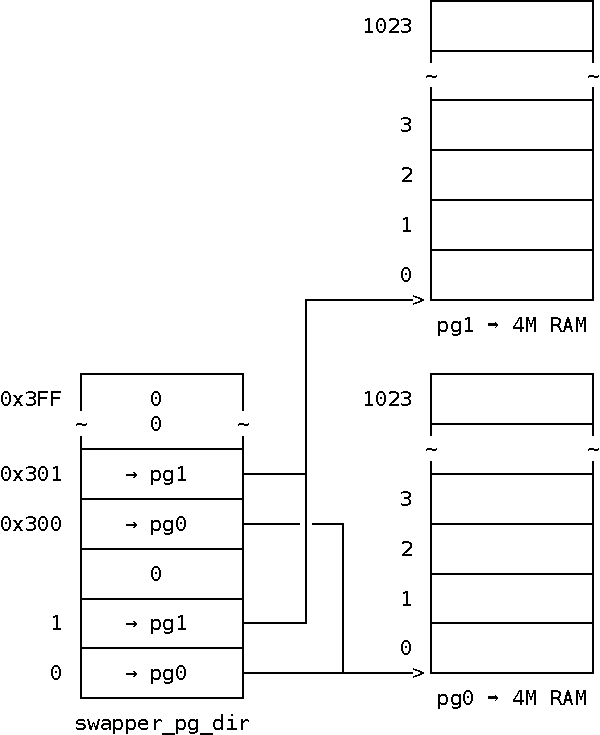
\includegraphics[width=.4\textwidth]{kernel-page-table-boot}
    \end{center}
    Therefore, the kernel must create a mapping from both the linear addresses
    \code{0x00000000} through \code{0x007fffff} (8M) and the linear addresses
    \code{0xc0000000} through \code{0xc07fffff} (8M) into the physical addresses
    \code{0x00000000} through \code{0x007fffff}. In other words, the kernel during its
    first phase of initialization can address the first 8 MB of RAM by either linear
    addresses identical to the physical ones or 8 MB worth of linear addresses, starting
    from \code{0xc0000000}.
    \begin{description}
    \item[Why?] (Sec 1.3.2, \emph{Provisional Kernel Page Tables}, \cite{abhishek2002memory})
      \begin{itemize}
      \item All pointers in the compiled kernel refer to addresses $> PAGE\_OFFSET$. That
        is, the kernel is linked under the assumption that its base address will be
        \code{start\_text} (I think; I don't have the code on hand at the moment), which
        is defined to be $PAGE\_OFFSET+(some\ small\ constant,\ call\ it\ C)$.
      \item All the kernel bootstrap code (mostly real mode code) is linked assuming that
        its base address is $0+C$.
      \end{itemize}

      \code{head.S} is part of the bootstrap code. It's running in protected mode with
      paging turned off, so all addresses are physical. In particular, the instruction
      pointer is fetching instructions based on physical address. The instruction that
      turns on paging (\code{movl \%eax, \%cr0}) is located, say, at some physical address
      \code{A}.

      As soon as we set the paging bit in \code{cr0}, paging is enabled, and starting at
      the very next instruction, all addressing, including instruction fetches, pass
      through the address translation mechanism (page tables). IOW, all address are
      henceforth virtual. That means that
      \begin{enumerate}
      \item We must have valid page tables, and
      \item Those tables must properly map the instruction pointer to the next instruction
        to be executed.
      \end{enumerate}
      That next instruction is physically located at address \code{A+4} (the address
      immediately after the "\code{movl \%eax, \%cr0}" instruction), but from the point of
      view of all the kernel code --- which has been linked at \code{PAGE\_OFFSET} ---
      that instruction is located at virtual address \code{PAGE\_OFFSET+(A+4)}. Turning on
      paging, however, does not magically change the value of EIP \footnote{The value of
        EIP is still physically \code{A+4}, not \code{PAGE\_OFFSET+(A+4)} yet. But since
        paging is just enabled, CPU could pass \code{A+4} through address translation.}.
      The CPU fetches the next instruction from ***virtual*** address \code{A+4}; that
      instruction is the beginning of a short sequence that effectively relocates the
      instruction pointer to point to the code at \code{PAGE\_OFFSET+A+(something)}.

      But since the CPU is, for those few instructions, fetching instructions based on
      physical addresses ***but having those instructions pass through address
      translation***, we must ensure that both the physical addresses and the virtual
      addresses are :
      \begin{enumerate}
      \item Valid virtual addresses, and
      \item Point to the same code.
      \end{enumerate}
      That means that at the very least, the initial page tables must
      \begin{enumerate}
      \item map virtual address \code{PAGE\_OFFSET+(A+4)} to physical address
        \code{(A+4)}, and must
      \item map virtual address \code{A+4} to physical address \code{A+4}.
      \end{enumerate}
      This dual mapping for the first 8MB of physical RAM is exactly what the initial page
      tables accomplish. The 8MB initally mapped is more or less arbitrary. It's certain
      that no bootable kernel will be greater than 8MB in size. The identity mapping is
      discarded when the MM system gets initialized.
    \end{description}
  \end{itemize}
  \begin{center}
    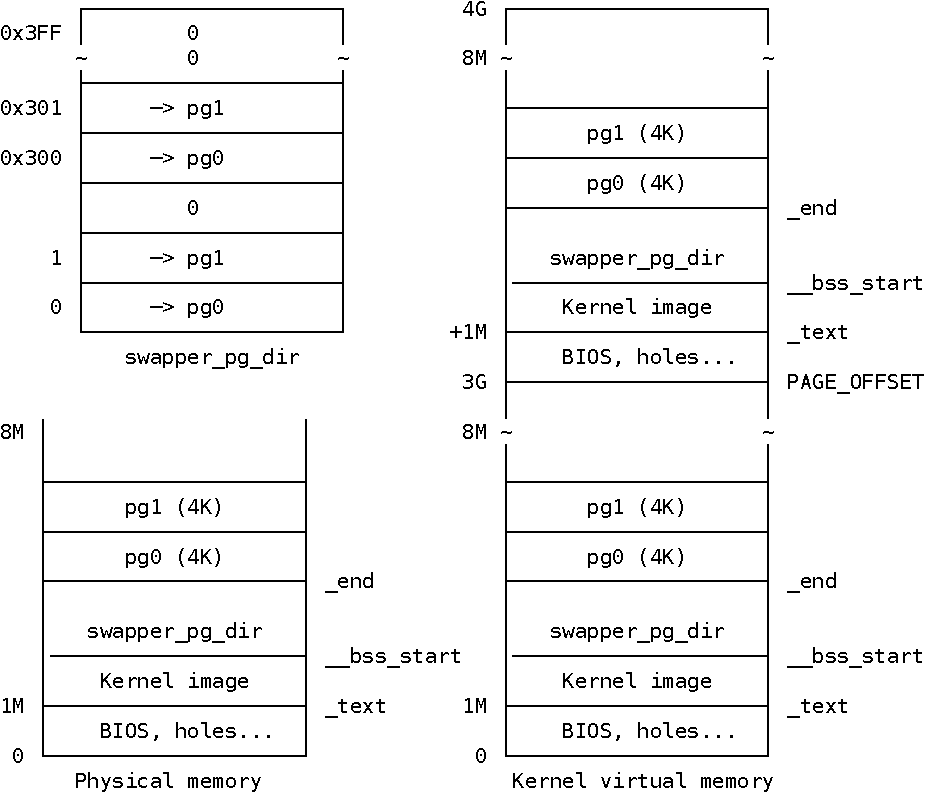
\includegraphics[width=.5\textwidth]{kernel-page-table}
  \end{center}
  line \href{http://lxr.linux.no/linux+v2.6.11/arch/i386/kernel/head.S#L91}{91-111} in
  \code{head.S}
    \begin{gascode}
page_pde_offset = (__PAGE_OFFSET >> 20);

        movl $(pg0 - __PAGE_OFFSET), %edi
        movl $(swapper_pg_dir - __PAGE_OFFSET), %edx
        movl $0x007, %eax                # 0x007 = PRESENT+RW+USER 
10:
        leal 0x007(%edi),%ecx            # Create PDE entry 
        movl %ecx,(%edx)                 # Store identity PDE entry 
        movl %ecx,page_pde_offset(%edx)  # Store kernel PDE entry 
        addl $4,%edx
        movl $1024, %ecx
11:
        stosl
        addl $0x1000,%eax
        loop 11b
        # End condition: we must map up to and including INIT_MAP_BEYOND_END 
        # bytes beyond the end of our own page tables; the +0x007 is the attribute bits 
        leal (INIT_MAP_BEYOND_END+0x007)(%edi),%ebp
        cmpl %ebp,%eax
        jb 10b
        movl %edi,(init_pg_tables_end - __PAGE_OFFSET)
      \end{gascode}
    \begin{center}
      \includegraphics[width=.5\textwidth]{i386pte}
    \end{center}
    \begin{itemize}
      % \item The identity mapping is discarded when the MM system gets initialized.
    \item \mint{gas}|page_pde_offset = (__PAGE_OFFSET >> 20); # 0xC00, the 3K point.|

      The \code{PGDir} is one page (4K) in size. It's divided into two parts:
      \begin{enumerate}
      \item first 3K (768 entries) for user mode
      \item last 1K (256 entries) for kernel mode
      \end{enumerate}
    \item \code{\$(pg0 - \_\_PAGE\_OFFSET)} yields the physical address of \code{pg0}
      since here it is a linear address. Same case for \code{\$(swapper\_pg\_dir -
        \_\_PAGE\_OFFSET)}.
      \begin{itemize}
      \item \code{swapper\_pg\_dir} starts at the beginning of BSS
      \item \code{pg0} starts at \code{\_end}
      \end{itemize}
    \item Registers:
      \begin{description}
      \item[\code{\%edi}] address of each page table entry, i.e. \code{pg0[0]..pg0[1023]},
        \code{pg1[0]..pg1[1023]}.
      \item[\code{\%edx}] address of \code{swapper\_pg\_dir[0]}, and then to
        \code{swapper\_pg\_dir[1]}.
      \item[\code{\%ecx}] has two uses
        \begin{enumerate}
        \item contents of \code{swapper\_pg\_dir[0]}, \code{swapper\_pg\_dir[1]},
          \code{swapper\_pg\_dir[768]},\\ \code{swapper\_pg\_dir[769]}.
        \item loop counter (1024 -> 0)
        \end{enumerate}
      \item[\code{\%eax}] \code{7, 4k+7, 8k+7 ... 8M-4k+7} for 2k page table entries in
        \code{pg0} and \code{pg1} respectively.
      \item[\code{\%ebp}] \code{= 128k + 7 + \&pg0[1023]} in the first round of loop. Its
        value cannot be determined at coding time, because the address of \code{pg0} is
        not known until compile/link time.
      \end{description}
    \item \code{stosl}: stores the contents of EAX at the address pointed by \code{EDI},
      and increments \code{EDI}. Equivalent to:
      \begin{enumerate}
      \item \code{movl \%eax, (\%edi)}
      \item \code{addl \$4, \%edi}
      \end{enumerate}
    \item \code{cmpl, jb}: if \code{\%eax} < \code{\%ebp}, jump to 10;
      \begin{itemize}
      \item \code{jb}:
        (\href{http://en.wikipedia.org/wiki/X86_assembly_language#Program_flow}{Wikipedia:
          x86 assembly language}) jump on below/less than, unsigned
      \item At the end of the 1\textsuperscript{st} round of loop, the value of
        \code{\%eax} is \code{4M-4k+7}, while the value of \code{\%ebp} depends on the
        address of \code{pg0}.

        If the kernel image is small enough (e.g. a \texttt{zImage}), \code{pg0} could be
        low enough to let the 128KB covered without a \code{pg1}.
      \end{itemize}
    \item \code{INIT\_MAP\_BEYOND\_END}: 128KB, used as a bitmap covering all pages. For
      1M pages (4GB RAM), we need 1M bits (128K
      bytes). (\url{http://kerneldiy.com/blog/?p=201})
    \end{itemize}
    \href{http://www.eefocus.com/article/09-04/71517s.html}{Equivalent pseudo C code}:
    \begin{center}
      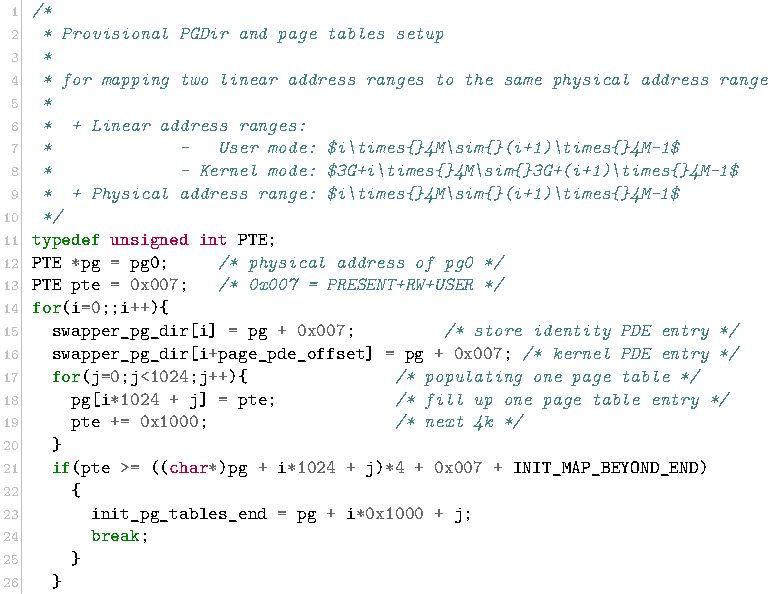
\includegraphics[width=.7\textwidth]{provisional-pgdir1}
    \end{center}
\item
  \href{http://tldp.org/HOWTO/Linux-i386-Boot-Code-HOWTO/kernel_head.html#enable_paging}{Linux
    HOWTO: Enable paging}
  (\href{http://lxr.linux.no/linux+v2.6.11/arch/i386/kernel/head.S#L186}{line 186-194 in
    \code{head.S}})
  \begin{center}
    
\includegraphics[width=.7\textwidth]{head6}
  \end{center}
\end{itemize}
    
% \begin{frame}{start\_of\_setup}
%   \begin{itemize}
%   \item sets up a stack
%   \item zeroes the bss segment
%   \item jumps to \code{main()} in \emph{arch/x86/boot/main.c}
%   \end{itemize}
% \end{frame}

% \begin{frame}{main()}
%   \code{main()} does some house keeping like detecting memory layout, setting a video mode,
%   etc. It then calls \code{go\_to\_protected\_mode()} in \emph{arch/x86/boot/pm.c}
% \end{frame}

% \begin{frame}{go\_to\_protected\_mode()}
%   \begin{itemize}
%   \item \code{enable\_a20()} --- addressing more than 1MB in real mode
%   \item \code{setup\_idt()}
%     \begin{itemize}
%     \item in real mode the \emph{interrupt vector table} is at address 0
%     \item in protected mode, let IDTR take care of it.
%     \end{itemize}
%   \item \code{setup\_gdt()} --- put GDT's address into GDTR.
%     \begin{itemize}
%     \item GDT is used for address translation (logical $\rightarrow$ linear) in protected mode
%     \end{itemize}
%   \item \code{protected\_mode\_jump()} in \emph{arch/x86/boot/pmjump.S}
%     \begin{itemize}
%     \item setting the PE (Protected Enabled) bit in the CR0 CPU register
%     \item jumping to the 32-bit kernel entry point (\code{startup\_32()} for compressed kernel)
%     \end{itemize}
%   \end{itemize}
% \end{frame}

\subsection{start\_kernel()}
\label{sec:start_kernel}

\begin{frame}
  \begin{block}{\code{start\_kernel()} --- a long list of calls to initialize various
      kernel subsystems and data structures}
    \begin{itemize}
    \item \code{sched\_init()} --- scheduler
    \item \code{build\_all\_zonelists()} --- memory zones
    \item \code{page\_alloc\_init()}, \code{mem\_init()} --- buddy
      system
    \item \code{trap\_init()}, \code{init\_IRQ()} --- IDT
    \item \code{time\_init()} --- time keeping
    \item \code{kmem\_cache\_init()} --- slab allocator
    \item \code{calibrate\_delay()} --- CPU clock
    \item \code{kernel\_thread()} --- The kernel thread for process 1
    \item login prompt
    \end{itemize}
  \end{block}
\end{frame}

% \begin{frame}{\code{rest\_init()}}
%   \code{rest\_init()} in \emph{init/main.c}
%   \begin{itemize}
%   \item \code{kernel\_thread()}
%     \begin{itemize}
%     \item \code{kernel\_thread()} $\rightarrow$ \code{kernel\_init()} $\rightarrow$ \code{init\_post()}
%       \begin{itemize}
%       \item \code{kernel\_init()} is responsible for initializing the remaining CPUs in the system
%       \item \code{init\_post()} tries to execute a user-mode process --- init starts running as
%         PID 1.
%       \end{itemize}
%     \item \code{schedule()}
%     \item \code{cpu\_idle()}
%     \end{itemize}
%   \end{itemize}
% \end{frame}

\begin{frame}{The Kernel Boot Process}
  \begin{center}
    \mode<beamer>{
      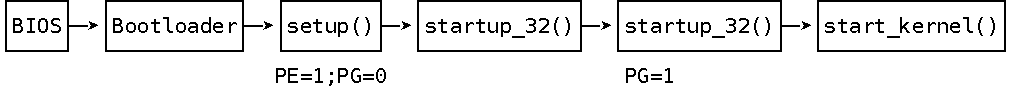
\includegraphics[height=.9\textheight]{bootprocess}
    }
    \mode<article>{
      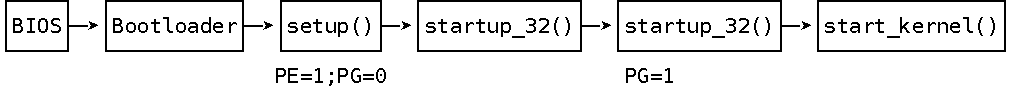
\includegraphics[height=.5\textheight]{bootprocess}
    }
  \end{center}
\end{frame}

\begin{frame}{The Kernel Boot Process (I)}
  \begin{center}
    \mode<beamer>{
      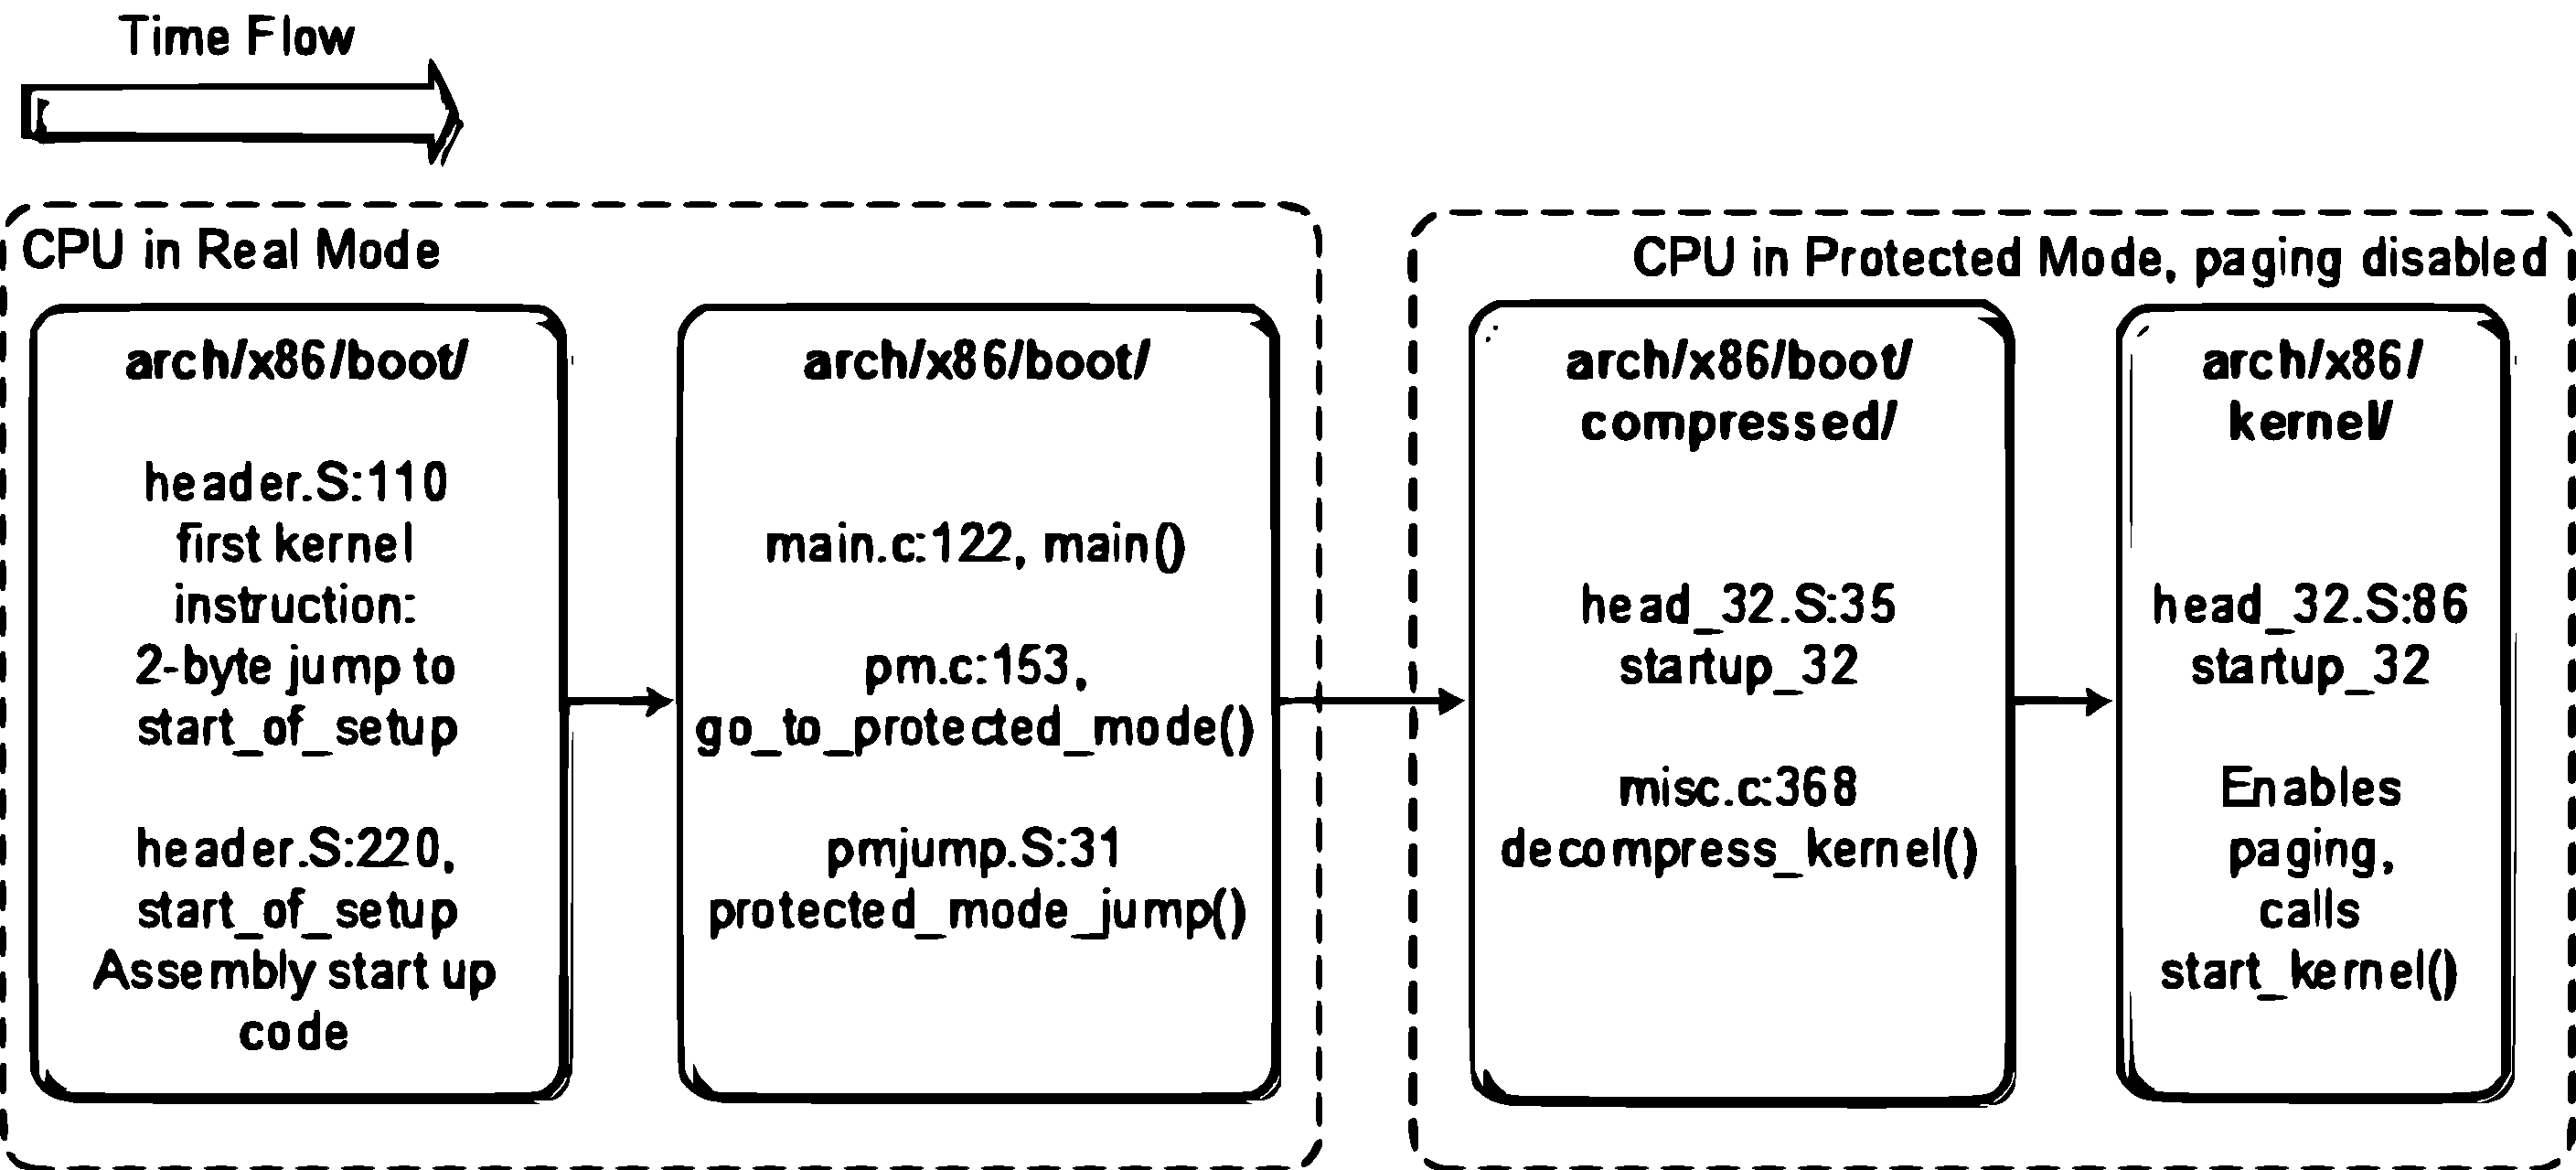
\includegraphics[width=\textwidth]{kernelInitPartOne}
    }
    \mode<article>{
      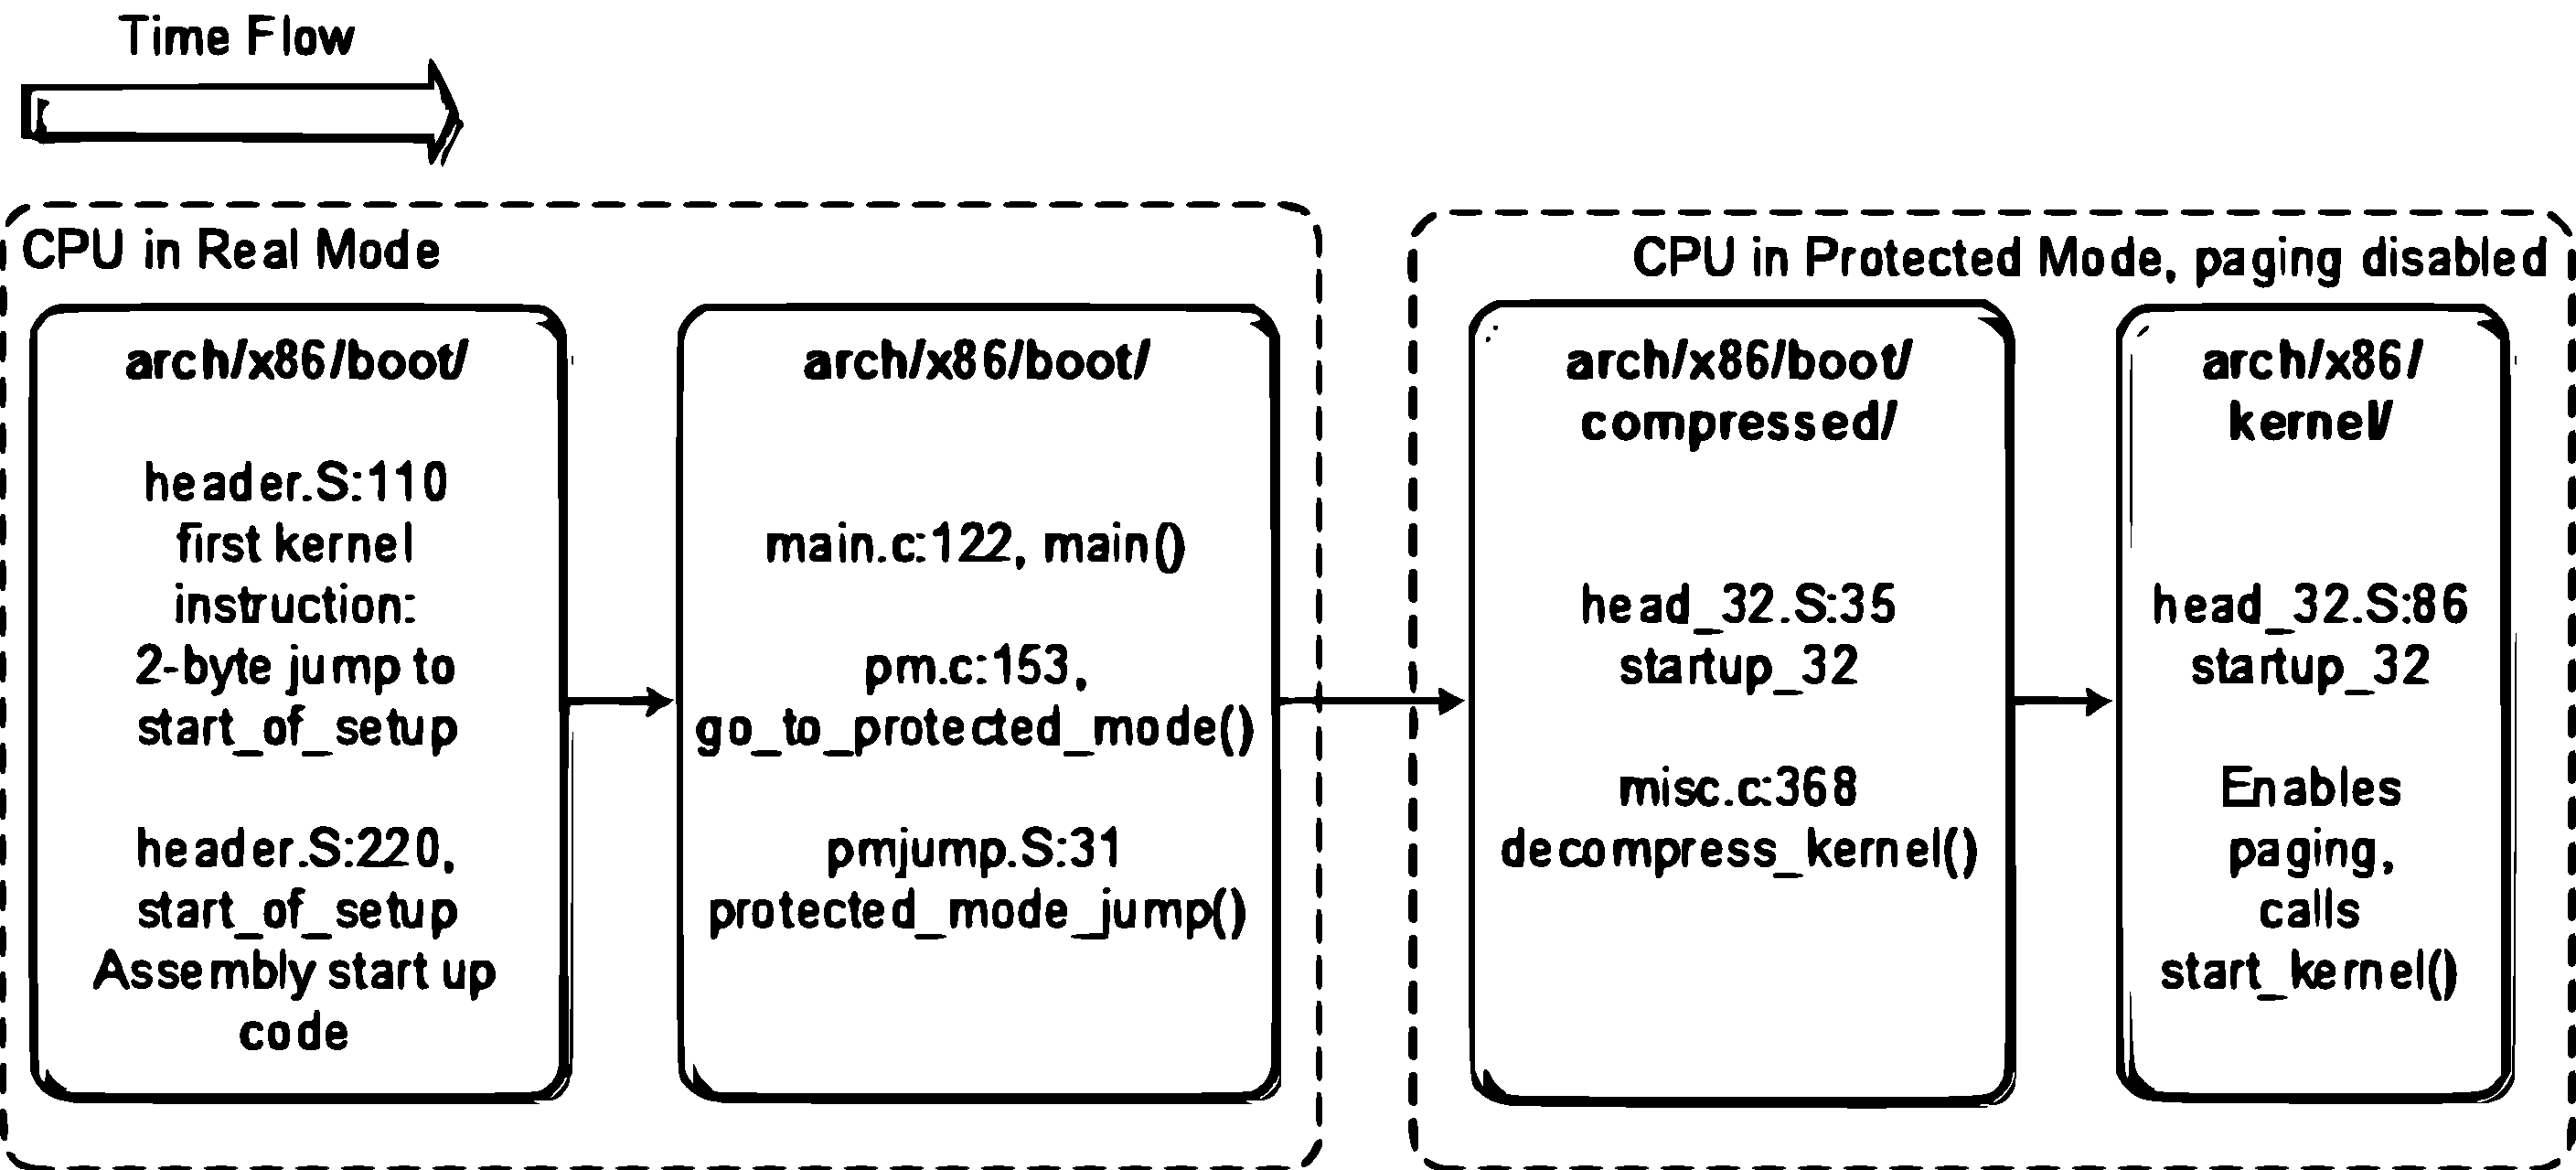
\includegraphics[width=.8\textwidth]{kernelInitPartOne}
    }
  \end{center}
\end{frame}

\begin{itemize}
\item This picture is not fully compatible with 2.6.11.
\end{itemize}

\begin{frame}{The Kernel Boot Process (II)}
  \begin{center}
    \mode<beamer>{
      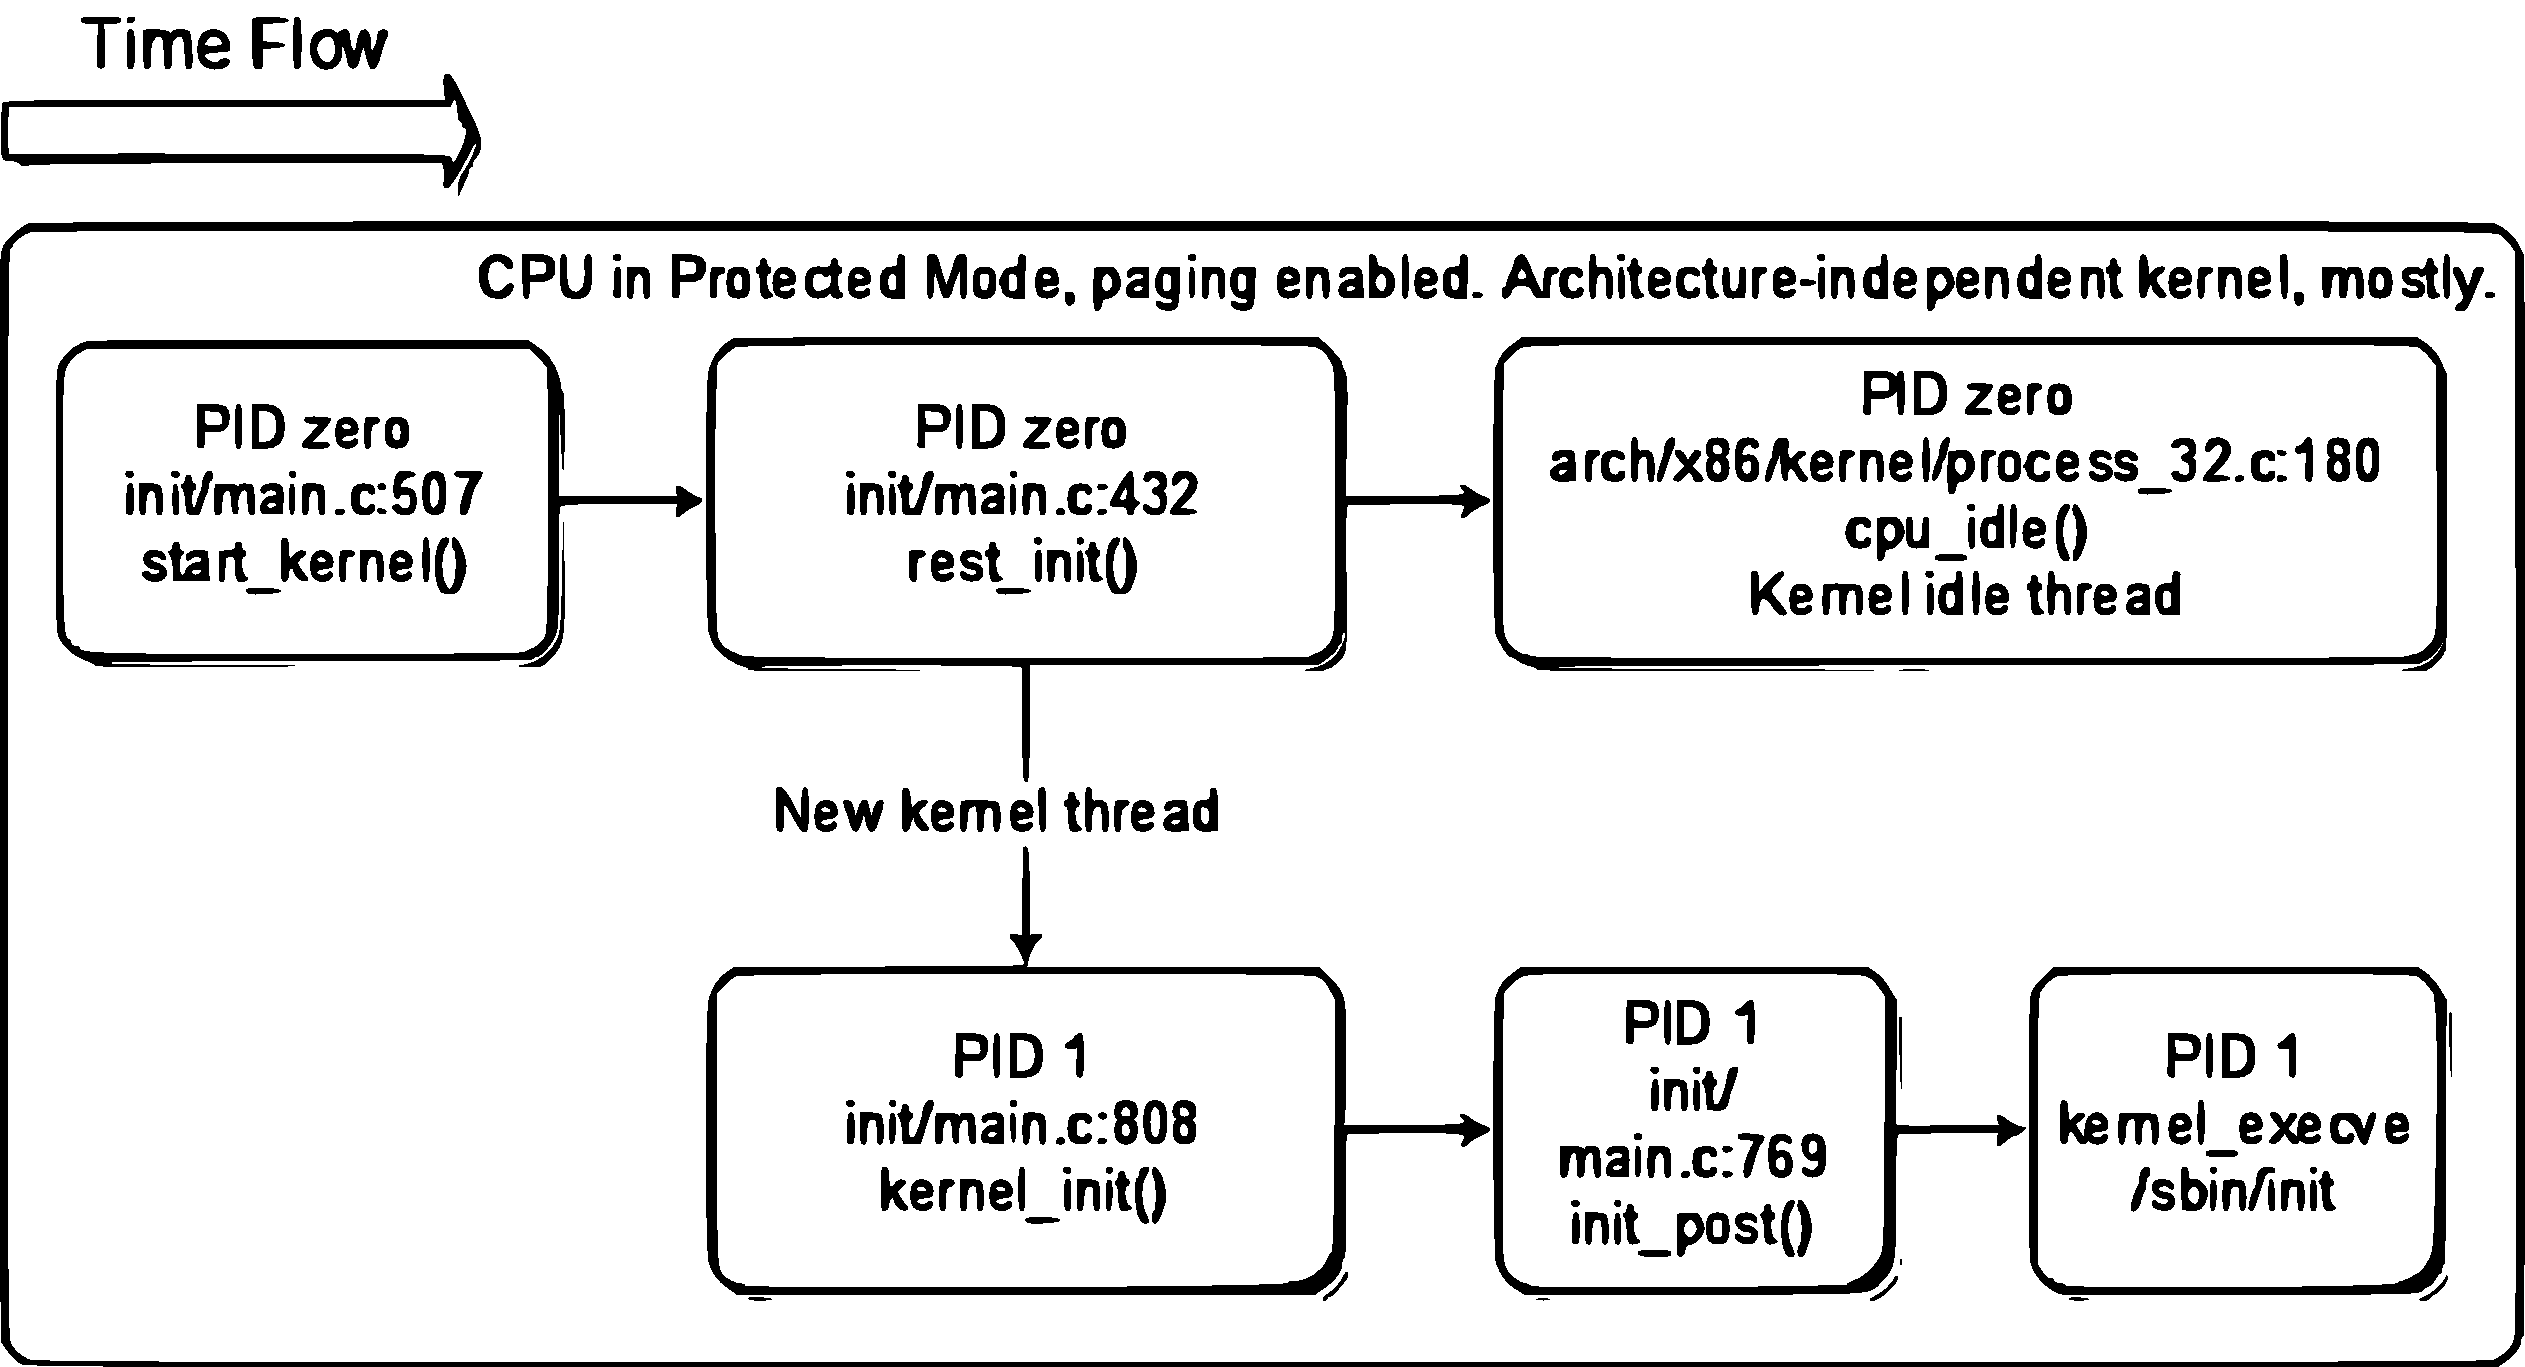
\includegraphics[width=\textwidth]{kernelInitPartTwo}
    }
    \mode<article>{
      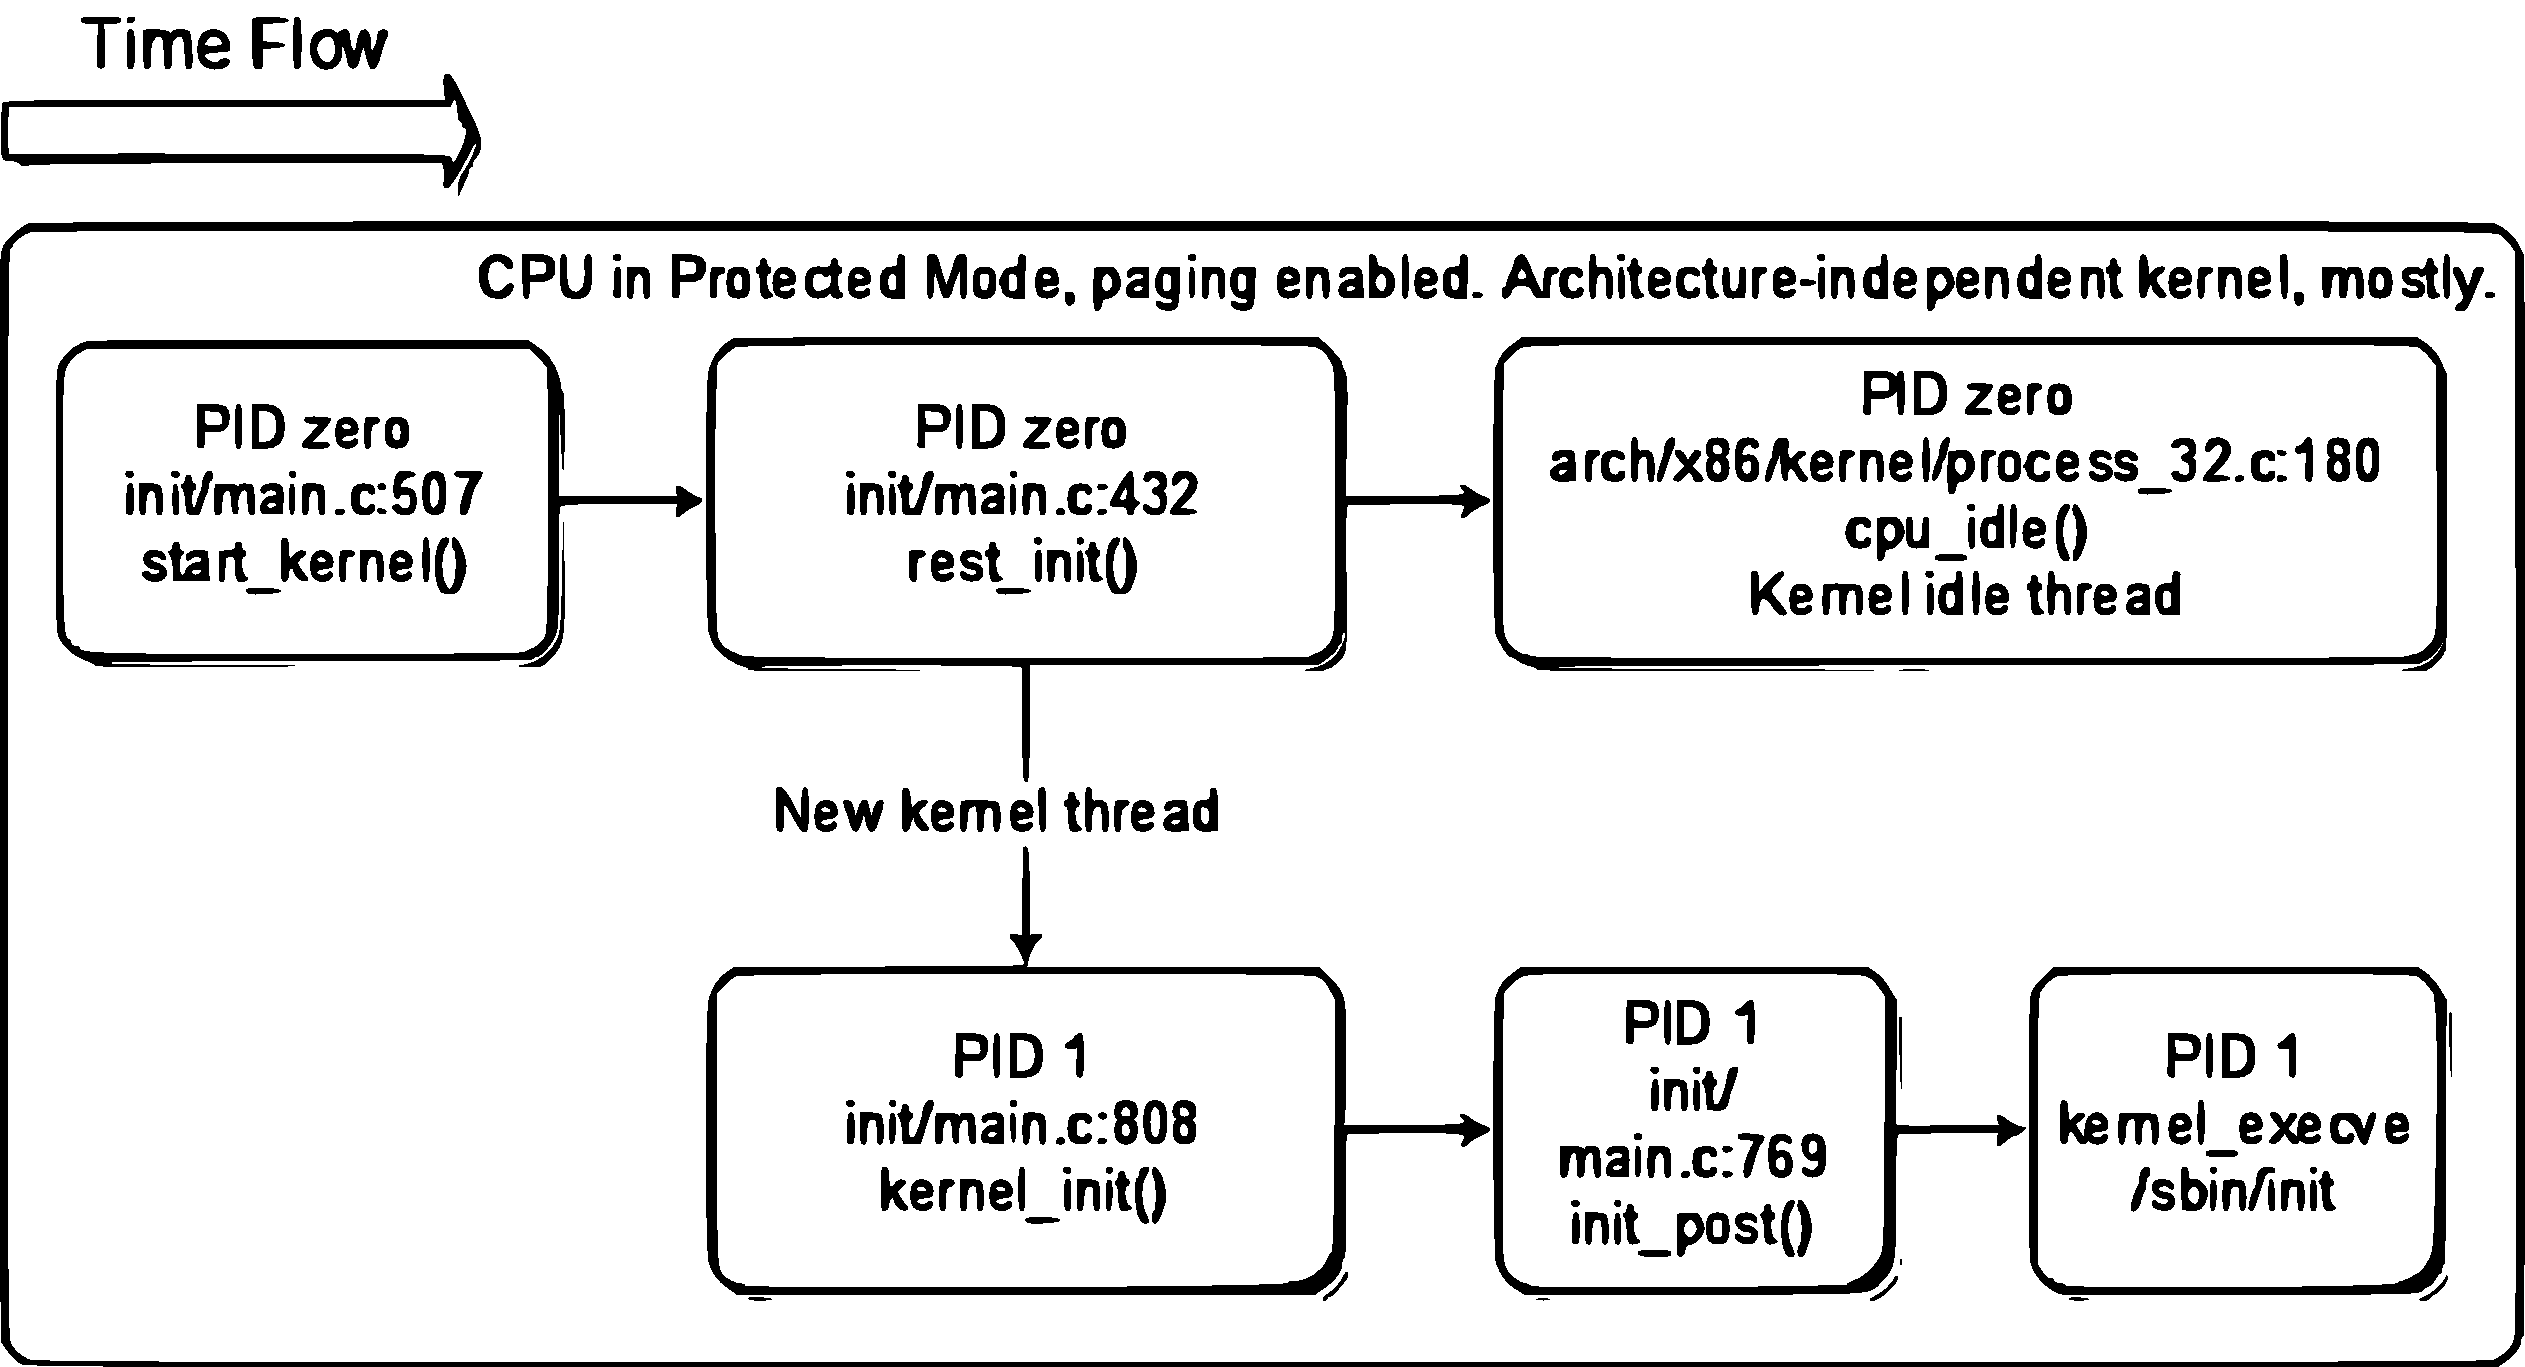
\includegraphics[width=.8\textwidth]{kernelInitPartTwo}
    }
  \end{center}
\end{frame}

\begin{itemize}
\item This picture is not fully compatible with 2.6.11.
\end{itemize}


% \begin{frame}[allowframebreaks]
%   \mode<beamer>{
%     \frametitle{References}
%     \documentclass[a4paper,10pt]{article}
\usepackage{beamerarticle}
\setjobnamebeamerversion{boot-b}

\usepackage{fullpage}

\usepackage[backend=biber,url=false,style=alphabetic]{biblatex}
\addbibresource{os.bib}

\usepackage{hyperref}
\usepackage[textsize=footnotesize]{todonotes}
\addtolength{\oddsidemargin}{-15pt}
\addtolength{\marginparsep}{5pt}
% \setlength{\marginparwidth}{1.2in}
% \let\oldmarginpar\marginpar
% \renewcommand\marginpar[1]{\-\oldmarginpar[\raggedleft\footnotesize #1]%
% {\raggedright\footnotesize #1}}
\newcommand{\Marginpar}[1]{\marginpar{\raggedright{\footnotesize \emph{#1}}}}

% http://tex.stackexchange.com/q/25259/86
% for *notes*
\defbeamertemplate<article>{frame begin}{lined}{
  \par\noindent\rule{\textwidth}{2pt}\par}
\defbeamertemplate<article>{frame end}{lined}{
  \par\vspace{1em}\noindent\rule{.1\textwidth}{.3pt}
  \raisebox{-3pt}{{\large \Info}}
  \rule{.1618\textwidth}{.3pt}\par\vspace{.5em}}

\setbeamertemplate{frame begin}[lined]
\setbeamertemplate{frame end}[lined]

%\documentclass[10pt,ignorenonframetext,xcolor=svgnames,hyperref={xetex,colorlinks,linkcolor=blue},compress]{beamer}

\usepackage{latexsym,pifont,units,amsmath,amsfonts,amssymb,marvosym}
\usepackage{xltxtra} %fontspec,xunicode are loaded here.
\defaultfontfeatures{Mapping=tex-text}
\setsansfont{DejaVu Sans}
\setmainfont{DejaVu Serif}

% \usepackage{graphicx} % beamer loads graphicx already.
\graphicspath{{./figs/}{../figs/}{./}{../}} %note that the trailing “/” is required

\usepackage{tikz}
\usetikzlibrary{arrows,decorations.pathmorphing,backgrounds,positioning,fit}

\usepackage{multicol,varwidth}

\usepackage{minted}
\renewcommand{\theFancyVerbLine}{
  \textcolor{lightgray}{\scriptsize \arabic{FancyVerbLine}}}

\newminted{gas}{ linenos=true,numbersep=2pt,fontsize=\footnotesize,
  frame=leftline,framesep=3pt,rulecolor=\color{lightgray}, xleftmargin=10pt }
\newminted{c}{ linenos=true,numbersep=2pt,fontsize=\footnotesize,
  frame=leftline,framesep=3pt,rulecolor=\color{lightgray}, xleftmargin=10pt }

\newcommand{\cfbox}[2]{%
  \colorlet{currentcolor}{.}%
  {\color{#1}\fbox{\color{currentcolor}#2}}%
}

\newcommand{\code}[1]{\texttt{\textcolor{violet}{#1}}}

\mode<beamer>{
  \usetheme{default}
  \usecolortheme{sidebartab}
  \usefonttheme{serif}
  \setbeamertemplate{footline}[frame number]
  \setbeamertemplate{navigation symbols}{}
  \usenavigationsymbolstemplate{}
  \setbeamertemplate{blocks}[rounded][shadow=true]
  \setbeamercolor{structure}{fg=Green}
  \setbeamercolor{block title}{fg=Green}
}

\begin{document}

\mode<article>{
  \title{From Power Up To Bash Prompt}
  \author{Wang Xiaolin\\wx672ster@gmail.com}
  \maketitle
  \tableofcontents
  \vspace{2em}
  \begin{description}
  \item[Textbook:]\
    \begin{itemize}
    \item Appendix A, \emph{System Startup}, \cite{bovet2005understanding}
    \item Appendix D, \emph{System Startup}, \cite{mauerer2008professional}
    \item Chapter 8, \emph{Booting the Kernel}, \cite{rodriguez2005linux}
    \end{itemize}
  \end{description}
  \printbibliography
  \clearpage
}

\begin{frame}<beamer>
    \title{From Power Up To Bash Prompt}
    \author{Wang Xiaolin}
    \titlepage
    \vfill
    \tiny{
      \ding{41} wx672ster+os@gmail.com
      % \ding{37} 13577067397
    }
\end{frame}

\section{Motherboard Chipsets And The Memory Map}
\label{sec:moth-chips-memory}

See \cite{gustavo2008chipsets}

\begin{frame}{Motherboard Chipsets And The Memory Map}
  \begin{center}
    \mode<beamer>{
      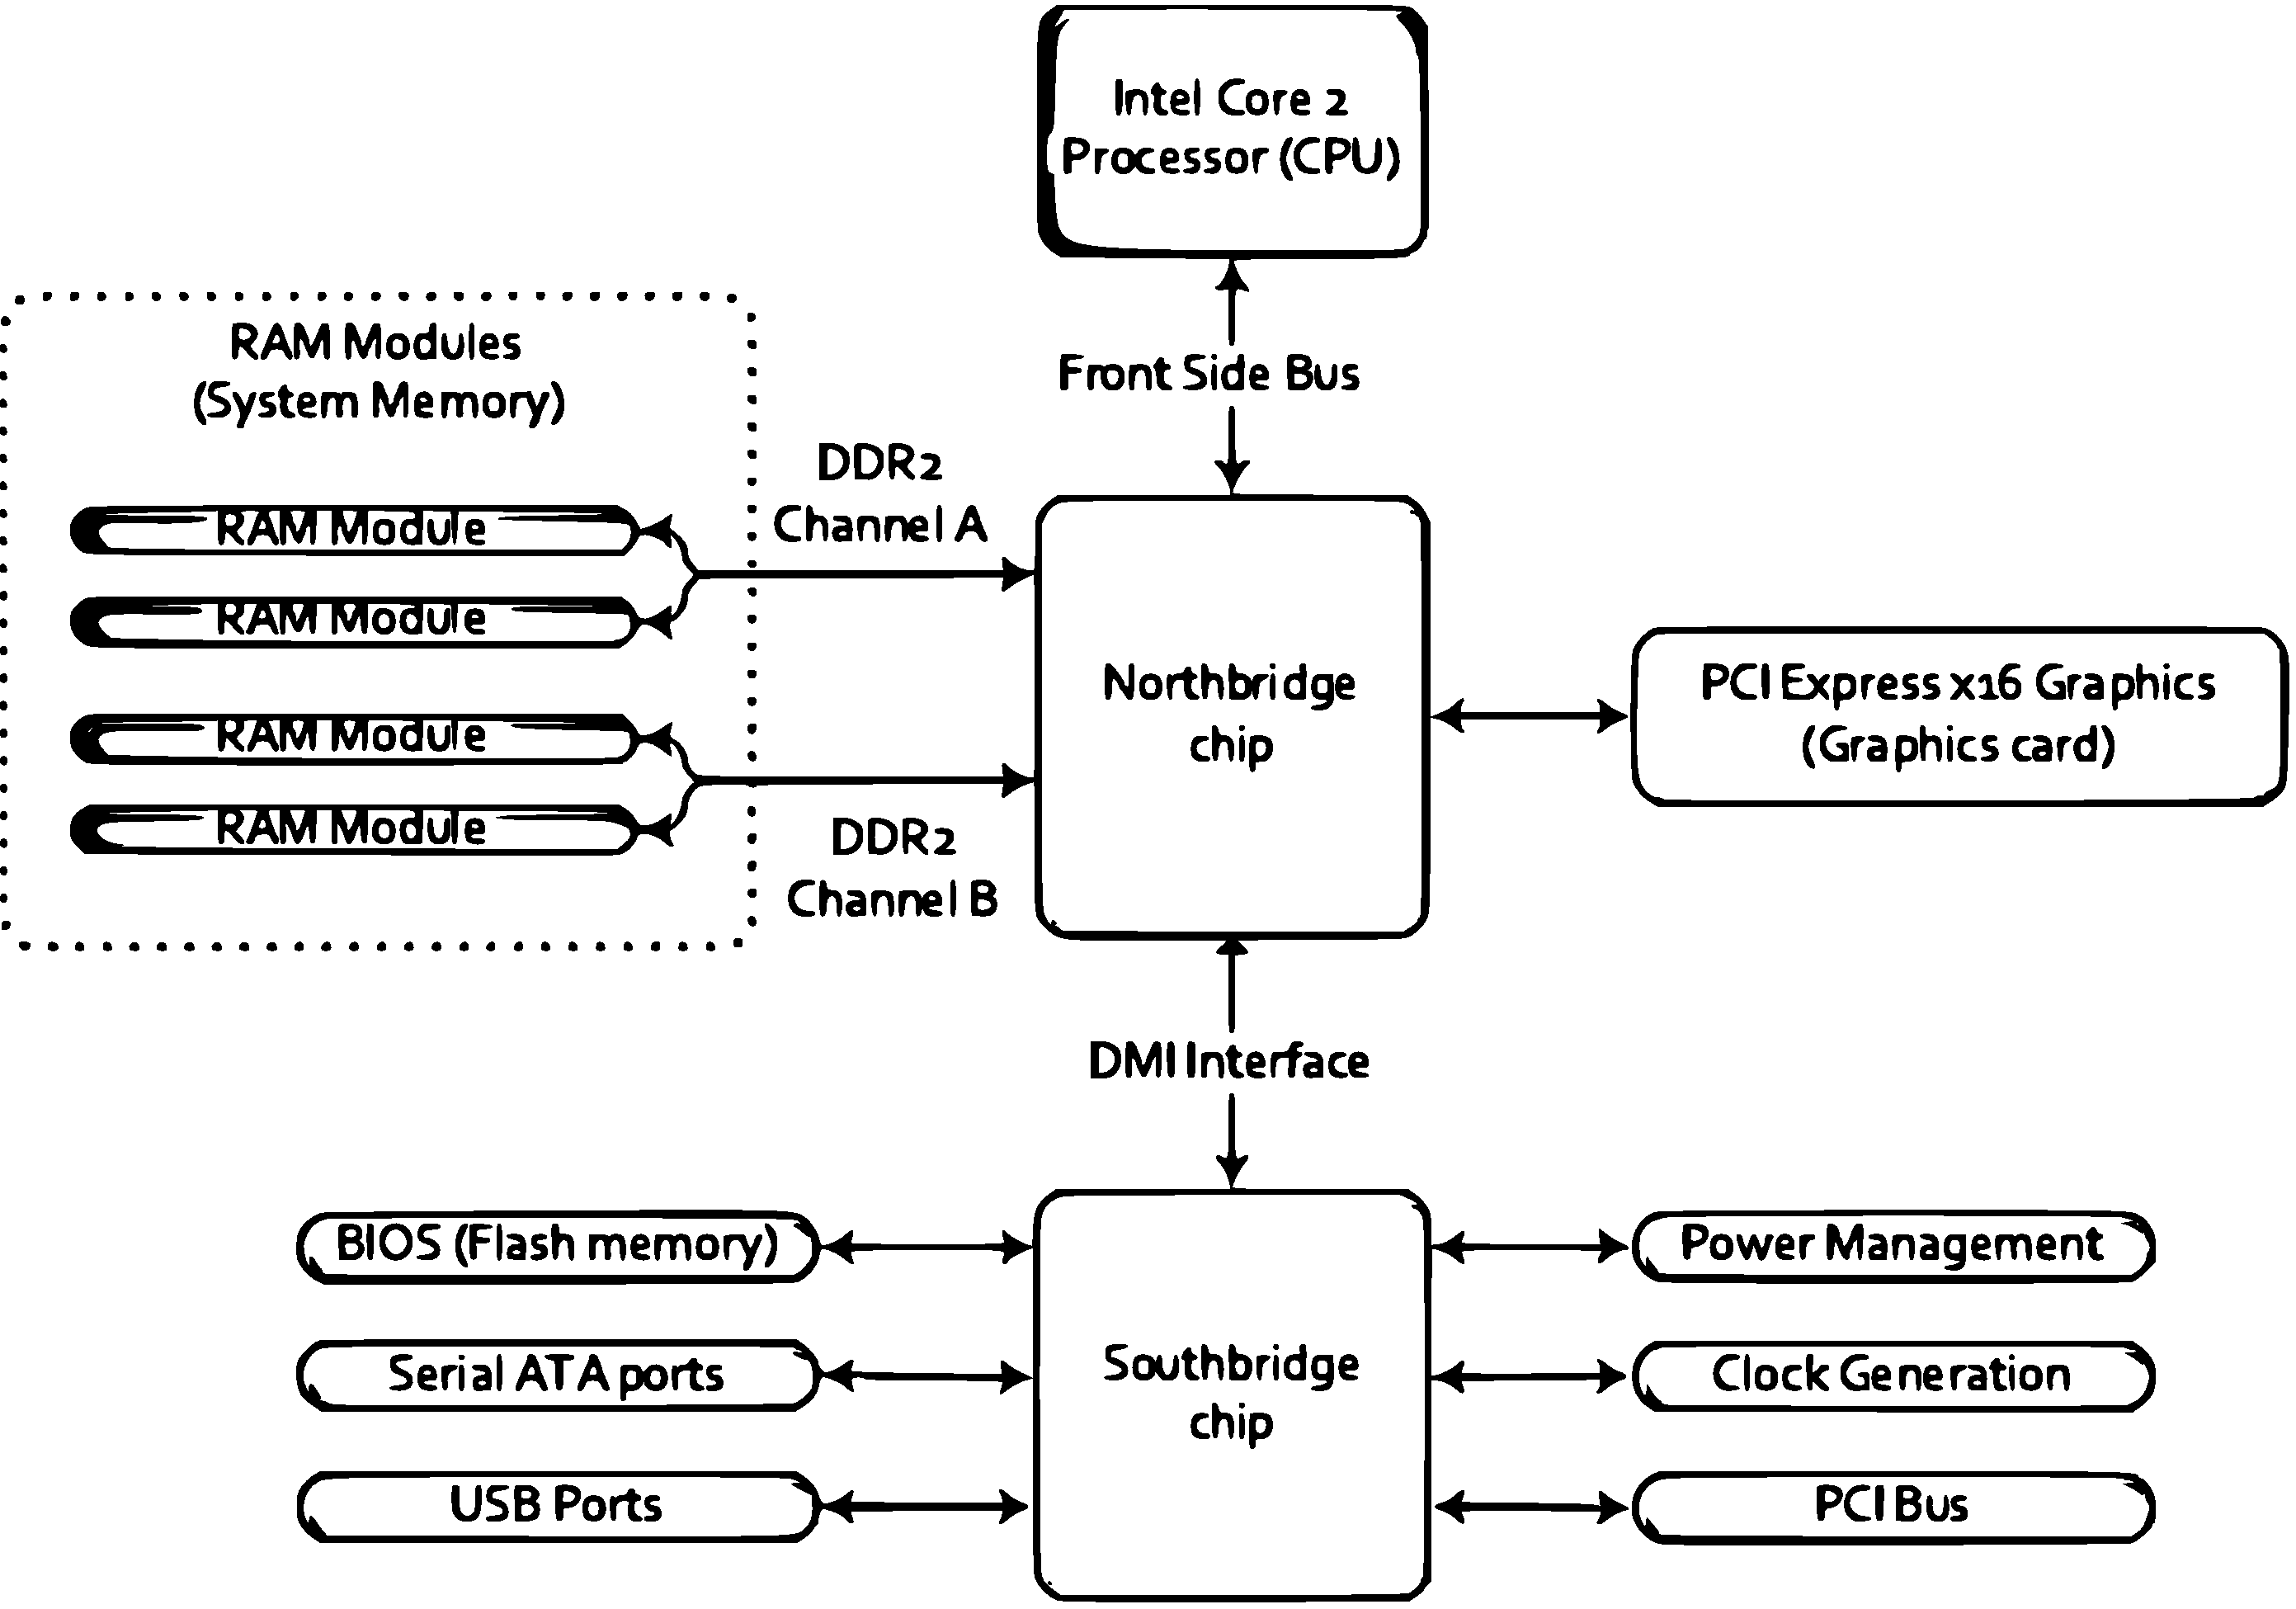
\includegraphics[width=\textwidth]{motherboardDiagram}
    }
    \mode<article>{
      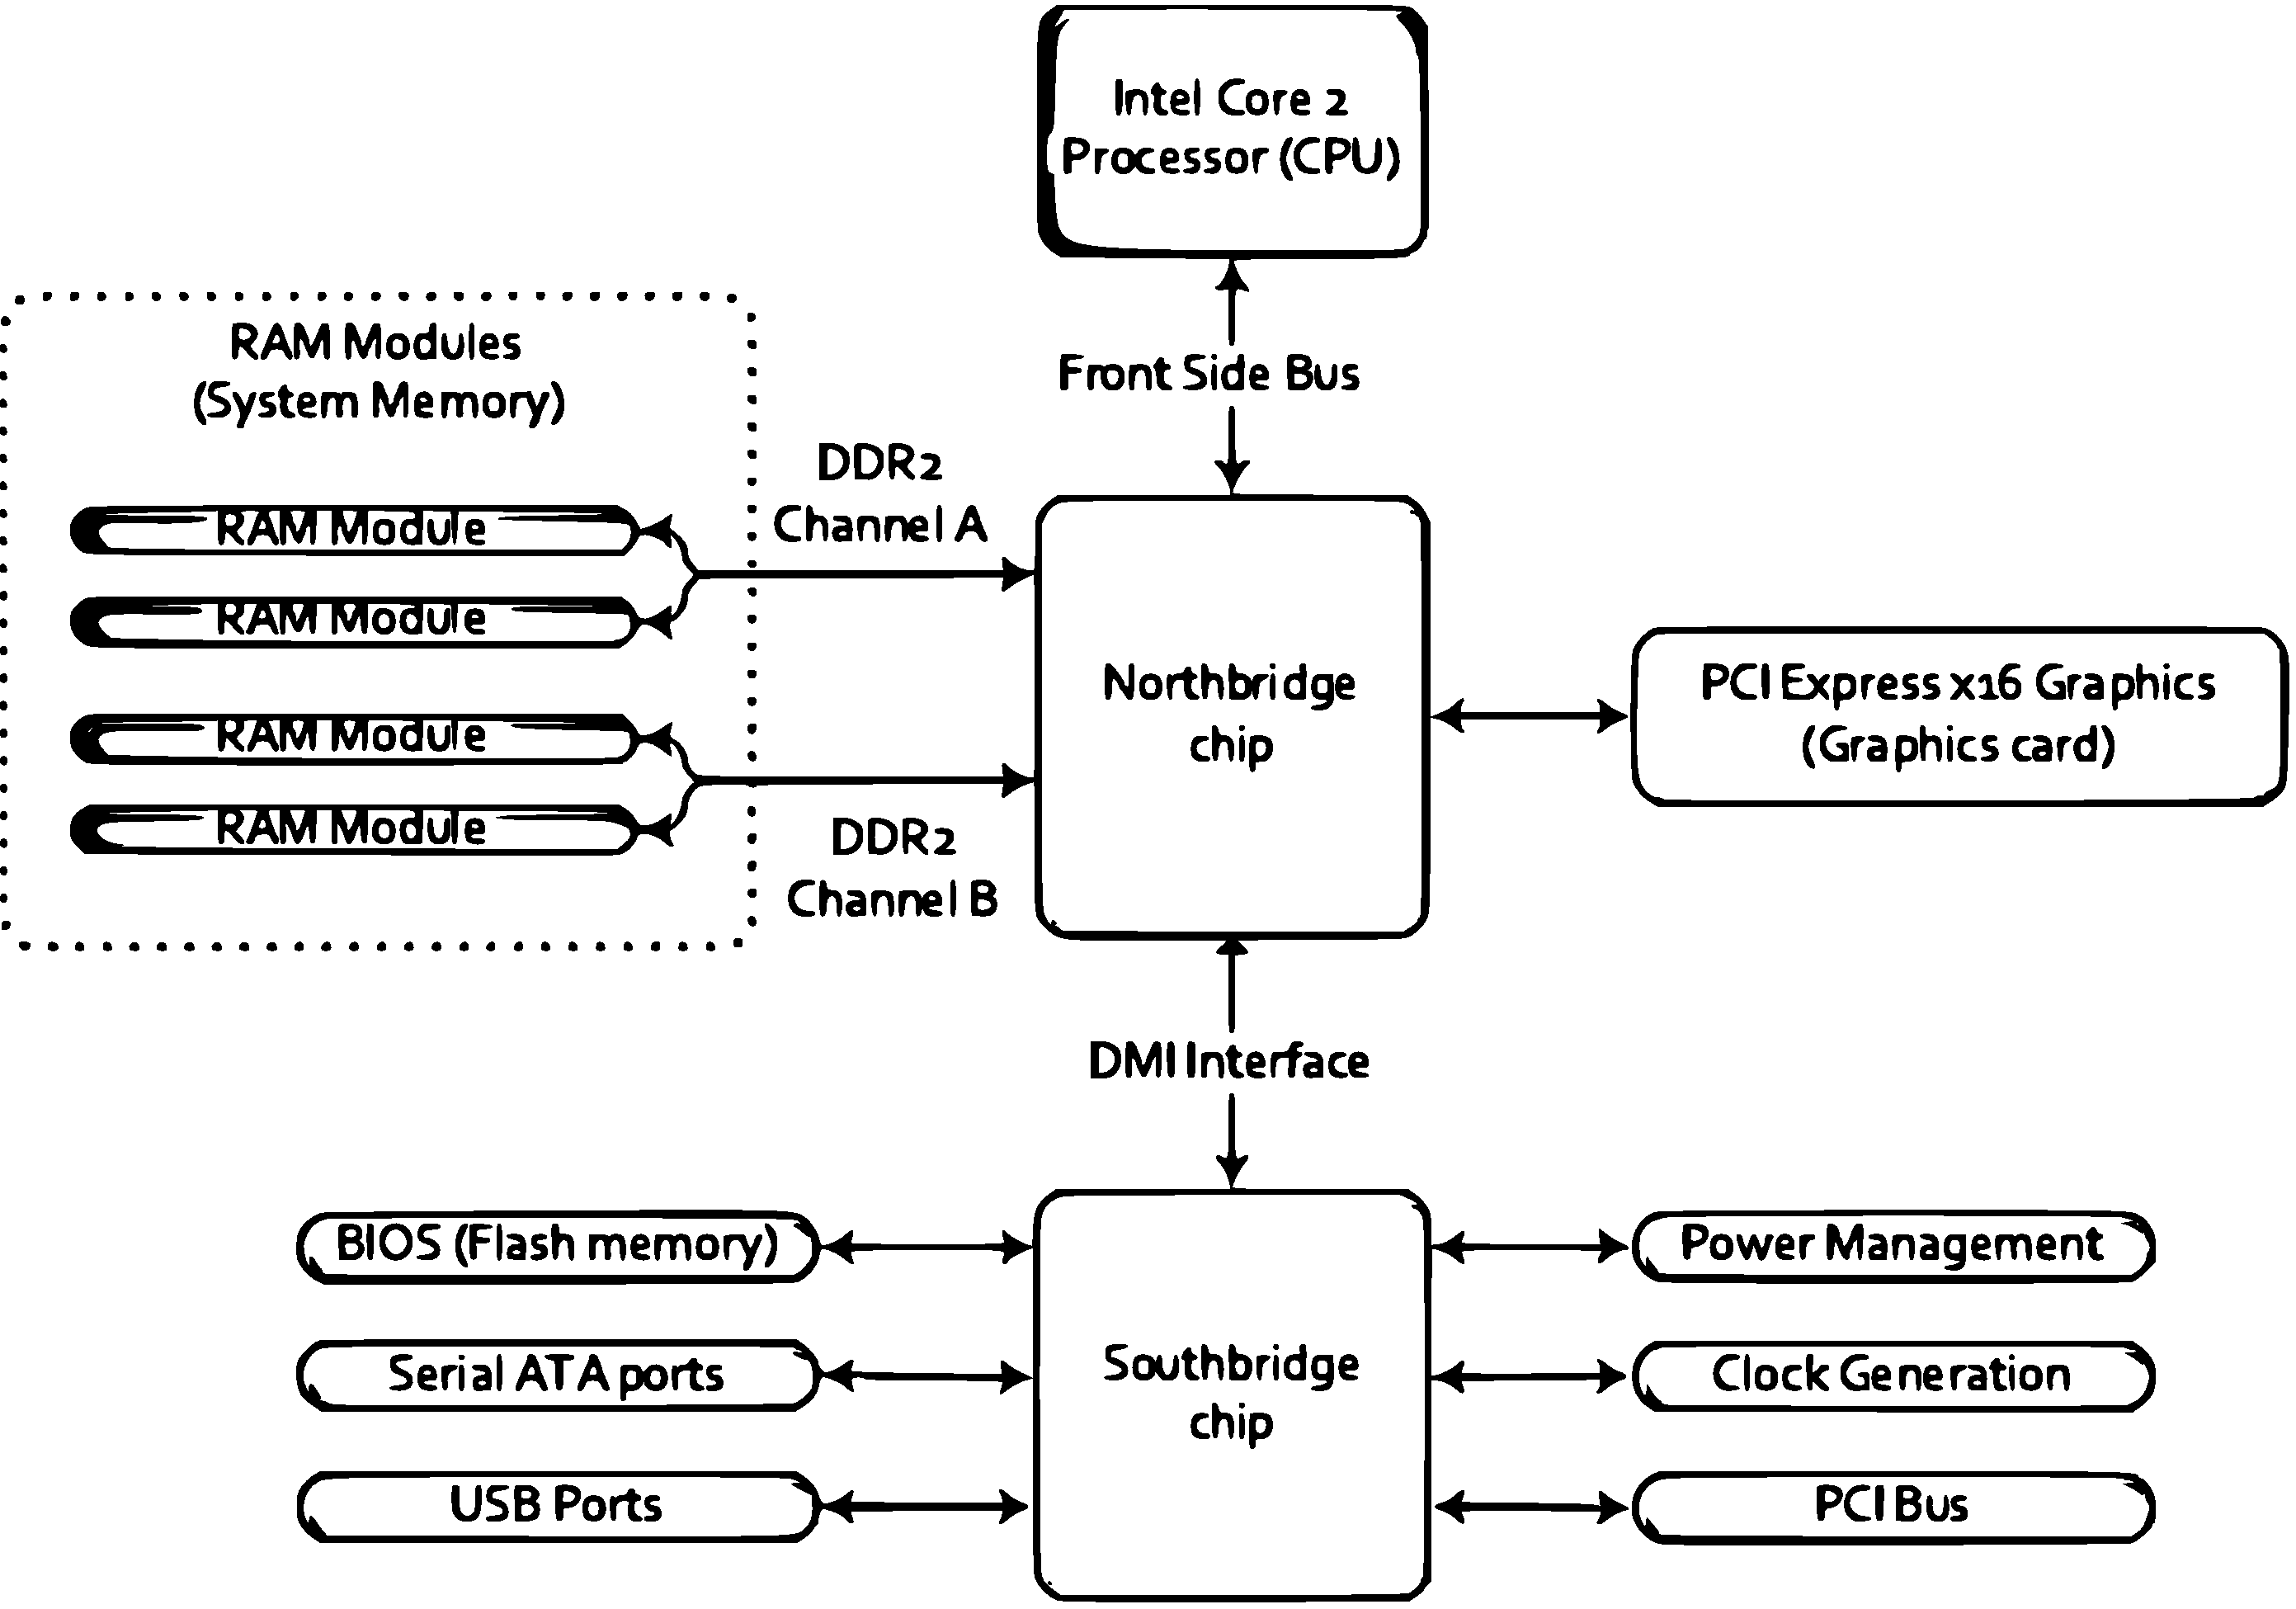
\includegraphics[width=.6\textwidth]{motherboardDiagram}
    }
  \end{center}
\end{frame}

\begin{frame}%{Motherboard Chipsets And The Memory Map}
  \begin{block}{Facts}
    \begin{itemize}
    \item The CPU doesn't know what it's connected to
      \begin{itemize}
      \item[-] CPU test bench?\quad{}network router?\quad{}toaster?\quad{}brain implant?
      \end{itemize}
    \item The CPU talks to the outside world through its pins
      \begin{itemize}
      \item[-] some pins to transmit the physical memory address
      \item[-] other pins to transmit the values
      \end{itemize}
    \item The CPU's gateway to the world is the front-side bus
    \end{itemize}
  \end{block}
  \begin{block}{Intel Core 2 QX6600}
    \begin{itemize}
    \item 33 pins to transmit the physical memory address
      \begin{itemize}
      \item[-] so there are $2^{33}$ choices of memory locations
      \end{itemize}
    \item 64 pins to send or receive data
      \begin{itemize}
      \item[-] so data path is 64-bit wide, or 8-byte chunks
      \end{itemize}
    \end{itemize}
    This allows the CPU to physically address 64GB of memory ($2^{33}\times{}8B$)
  \end{block}
\end{frame}

More info:
\begin{itemize}
\item \href{http://download.intel.com/design/processor/datashts/31559205.pdf}{Datasheet for Intel Core 2 Quad-Core Q6000 Sequence}
\end{itemize}

\begin{frame}%{Motherboard Chipsets And The Memory Map}{ --- Facts}
  \begin{varwidth}{.59\textwidth}
    \textcolor{blue}{Some physical memory addresses are mapped away!}
    \begin{itemize}
    \item only the addresses, not the spaces
    \item Memory holes
      \begin{itemize}
      \item[-] $640KB \sim 1MB$
      \item[-] /proc/iomem
      \end{itemize}
    \item Memory-mapped I/O
      \begin{itemize}
      \item BIOS ROM
      \item video cards
      \item PCI cards
      \item ...
      \end{itemize}
    \end{itemize}
    This is why 32-bit OSes have problems using 4G of RAM.
  \end{varwidth}\hfill
  \begin{varwidth}{.39\textwidth}
    \begin{center}
      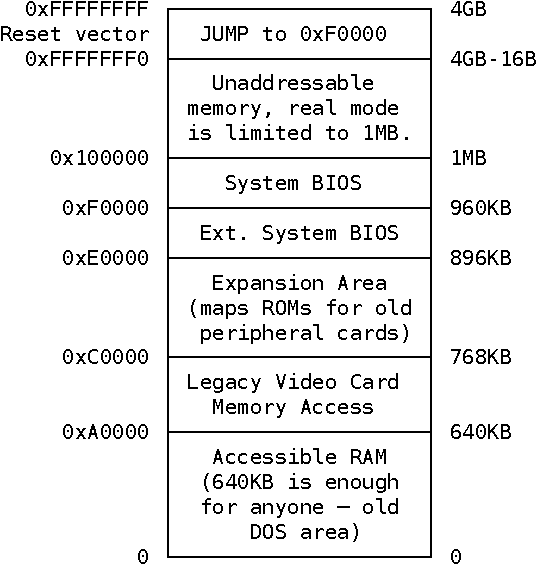
\includegraphics[width=1.2\textwidth]{boot-mem}
    \end{center}
  \end{varwidth}
  \vspace{1em}
  \begin{center}
    What if you don't have 4G RAM?
  \end{center}
\end{frame}

\begin{itemize}
\item \href{http://wiki.osdev.org/Memory_Map_(x86)}{OSDev: Memory Map (x86)}
\end{itemize}

\begin{frame}%{Motherboard Chipsets And The Memory Map}{ --- Facts}
  \begin{block}{the northbridge}
    \begin{enumerate}
    \item receives a physical memory request
    \item decides where to route it
      \begin{itemize}
      \item[-] to RAM? to video card? to ...?
      \item[-] decision made via the \emph{memory address map}
        \begin{itemize}
        \item \code{/proc/iomem}
        \item it is built in \code{setup()}
        \end{itemize}
      \end{itemize}
    \end{enumerate}
  \end{block}
\end{frame}

% \begin{itemize}
% \item When is the memory address map built? \code{setup()}.
% \end{itemize}

\begin{frame}%{Motherboard Chipsets And The Memory Map}{ --- Facts}
  \begin{block}{The CPU modes}
    \begin{description}
    \item[real mode:] CPU can only address 1MB RAM
      \begin{itemize}
      \item 20-bit address, 1-byte data unit
      \end{itemize}
    \item[32-bit protected mode:] can address 4GB RAM
      \begin{itemize}
      \item 32-bit address, 1-byte data unit
      \end{itemize}
    \item[64-bit protected mode:] can address 64GB RAM (Intel Core 2 QX6600)
      \begin{itemize}
      \item 33 address pins, 8-byte data unit
      \end{itemize}
    \end{description}
  \end{block}
  \begin{center}
    \$ \code{grep 'address sizes' /proc/cpuinfo}
  \end{center}
\end{frame}

\begin{itemize}
\item In the comments of
  \href{http://duartes.org/gustavo/blog/post/motherboard-chipsets-memory-map}{Motherboard
    Chipsets and the Memory Map}
  \begin{quote}
    The \emph{physical} stuff is determined by hard-core limits: the actual metal pins
    that stick out of the processor. It is \emph{those} pins that limit the CPU to 64
    gigabytes. That is completely independent of the operating system or even the mode
    (real-mode, 32-bit protected, 64-bit) the CPU is running in. It’s a physical
    limit. That is the limit for which that little multiplication is done. There are 33
    metal pins to transmit an address and 8 metal pins to send and receive data. So
    $2^{33}\times{} 2^3 = 2^{36} = 64 GB$.  The “unit” of transfer in this case is 8
    bytes, that’s the smallest chunk of data the CPU can address on the physical bus. In
    actuality, the CPU usually works in terms of cache lines, which hold 64 bytes in the
    Core 2s. Due to performance, the CPU reads a whole cache line at a time. So if a
    program reads one byte, the CPU actually reads 64 bytes and stores them in the cache.
    The 4-gb limit is logical, not physical. It happens because the registers and
    instructions in the CPU are limited to 32 bits \emph{when it’s running in 32-bit
      mode}, which \emph{does} depend on the OS. Programs need to be able to address
    individual bytes in memory, so the “unit” of addressing is 1 byte. So \emph{that}
    equation becomes $2^{32}\ addresses \times{} 1\ byte\ chunks = 2^{32}\ bytes$, or 4 GB
    total addressing.
  \end{quote}
\end{itemize}

\section{How Computers Boot Up}
\label{sec:how-computers-boot}

See \cite{gustavo2008boot}

\begin{frame}{Bootstrapping}
  \begin{center}
    \mode<beamer>{
      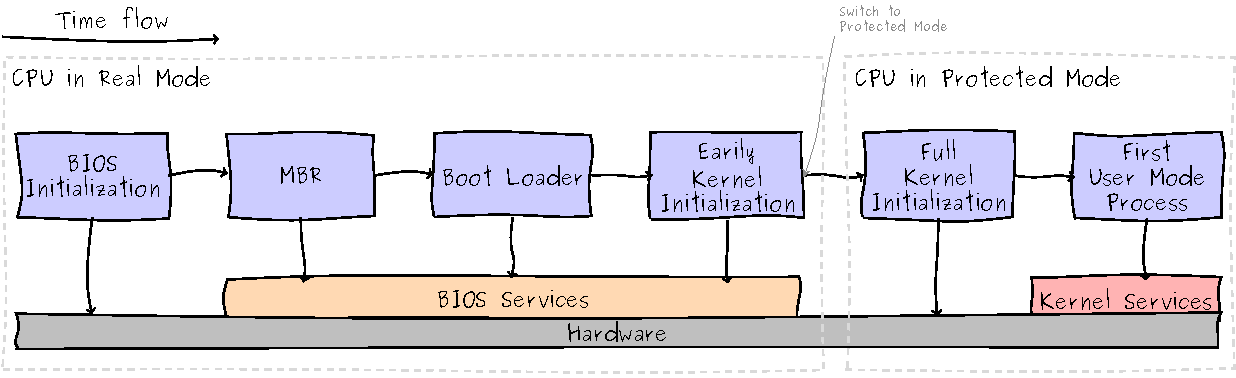
\includegraphics[width=\textwidth]{boot}
    }
    \mode<article>{
      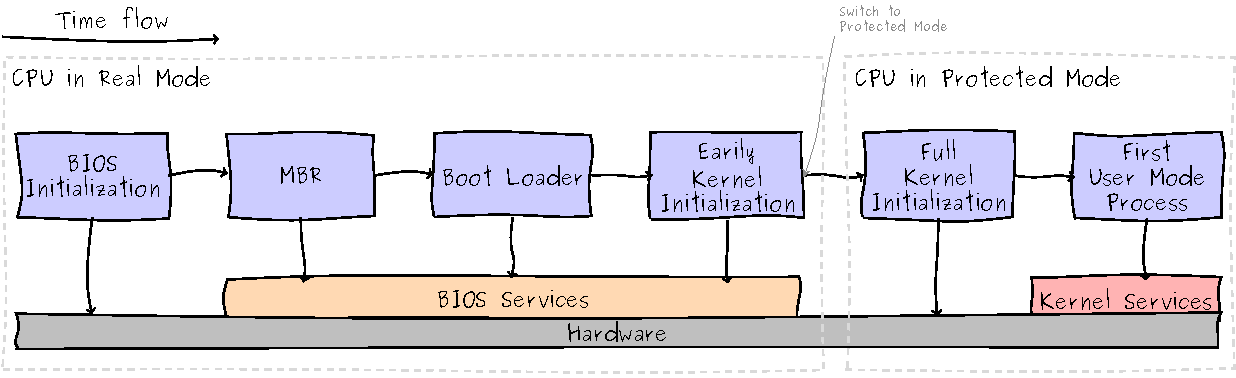
\includegraphics[width=.8\textwidth]{boot}
    }
  \end{center}
  \begin{enumerate}
  \item bringing at least a portion of the OS into main memory, and
  \item having the processor execute it
  \item the initialization of kernel data structures
  \item the creation of some user processes, and
  \item the transfer of control to one of them
  \end{enumerate}
  \begin{center}
    \code{man 7 boot}
  \end{center}
\end{frame}

\subsection{Motherboard power up}
\label{sec:motherboard-power-up}

\begin{frame}
  \begin{block}{Motherboard power up}
    \begin{enumerate}
    \item initializes motherboard firmwares (chipset, etc.)
    \item gets CPU running
    \end{enumerate}
  \end{block}
\end{frame}

\begin{frame}{Real mode}{ --- CPU acts as a 1978 Intel 8086}
  \begin{varwidth}{.52\textwidth}
    \begin{itemize}
    \item any code can write to any place in memory
    \item only 1MB of memory can be addressed
    \item registers are initialized
      \begin{itemize}
      \item[-] \code{EIP} has \code{0xFFFFFFF0}, the \textcolor{blue}{reset vector}
      \item[-] at the reset vector, there is a \code{jump} instruction, jumping to the
        \emph{BIOS entry point} (\code{0xF0000}).%\ (960KB)$, 64KB below 1MB)
      \end{itemize}
    \end{itemize}
  \end{varwidth}\hfill
  \begin{varwidth}{.48\textwidth}
    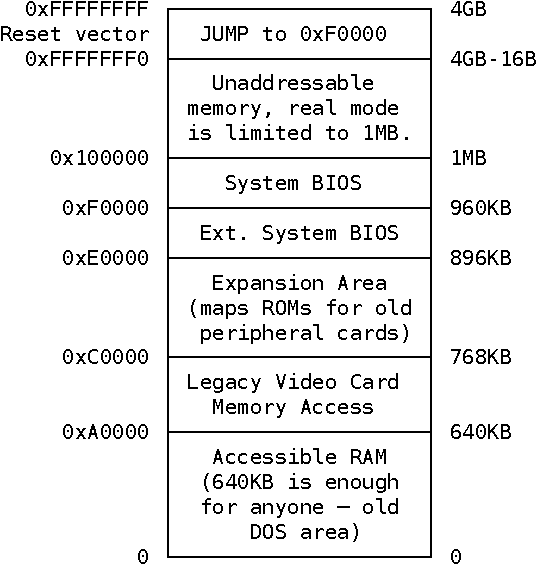
\includegraphics[width=1.15\textwidth]{boot-mem}
  \end{varwidth}
\end{frame}

More info:
\begin{itemize}
\item
  \href{http://stackoverflow.com/questions/7804724/how-is-the-bios-rom-mapped-into-address-space-on-pc}{stackoverflow:
    How is the BIOS rom mapped into address space on PC?}
\item \href{http://www.pcguide.com/ref/mbsys/bios/bootSequence-c.html}{The PC Guide: System
    Boot Sequence}
\item
  \href{http://stackoverflow.com/questions/5300527/do-normal-x86-or-amd-pcs-run-startup-bios-code-directly-from-rom-or-do-they-cop}{stackoverflow:
    Do normal x86 or AMD PCs run startup/BIOS code directly from ROM, or do they copy it
    first to RAM?}
\item \href{http://en.wikipedia.org/wiki/Reset_vector}{Wikipedia: Reset vector}
\item \href{http://lateblt.tripod.com/bit68.txt}{What Happens When A CPU Starts}
\item \href{http://www.freebsd.org/doc/en/books/arch-handbook/boot-bios.html}{FreeBSD:
    BIOS POST}
\item \href{http://www.freebsd.org/doc/en/books/arch-handbook/boot.html}{FreeBSD:
    Bootstrapping and Kernel Initialization}
\end{itemize}

\subsection{BIOS}
\label{sec:bios}

\begin{frame}{BIOS}
  \begin{block}{BIOS uses Real Mode addresses}
    \begin{itemize}
    \item No GDT, LDT, or paging table is needed
      \begin{itemize}
      \item the code that initializes the GDT, LDT, and paging tables must run in Real Mode
      \end{itemize}
    \item Real mode address translation:
      $$\text{segment number}\times{}2^4+offset$$
      \begin{itemize}
      \item[e.g.] to translate \code{<FFFF:0001>} into physical address:
        $$FFFF \times{} 16 + 0001 = FFFF0 + 0001 = FFFF1$$
      \item[if:] \code{offset > 0xF} (overflow)
      \item[then:] \code{address \% $2^{20}$} (wrap around)
      \item only 80286 and later x86 CPUs can address up to:
        $$FFFF0 + FFFF = 10FFEF$$
      \end{itemize}
    \end{itemize}
  \end{block}
\end{frame}

\begin{itemize}
\item \href{http://en.wikipedia.org/wiki/Real_mode}{Wikipedia: Real mode}
\item \href{http://wiki.osdev.org/Real_Mode}{OSDev: Real Mode}
\end{itemize}

\begin{frame}{CPU starts executing BIOS code}
  \begin{enumerate}
  \item POST
    \begin{itemize}
    \item an ACPI-compliant BIOS builds several tables that describe the hardware devices
      present in the system
    \end{itemize}
  \item initializes hardwares
    \begin{itemize}
    \item at the end of this phase, a table of installed PCI devices is displayed
    \end{itemize}
  \item find a boot device
  \item load MBR into \code{0x7c00}
  \item Jump to \code{0x7c00}
  \item MBR moves itself away from \code{0x7c00} (fig~\ref{boot-mem3})
  \end{enumerate}
  \begin{center}
    \mode<beamer>{
      \includegraphics[width=\textwidth]{mbr}
    } \mode<article>{
      \includegraphics[width=.7\textwidth]{mbr}
    }
  \end{center}
\end{frame}

\begin{varwidth}{.65\textwidth}
  \begin{itemize}
  \item The MBR includes a small boot loader, which is loaded into RAM starting from
    address \code{0x00007c00} by the
    BIOS. (\href{http://www.glamenv-septzen.net/en/view/6}{Why \code{0x7c00}}?)
  \item This small program moves itself to the address \code{0x00096a00}, sets up the Real
    Mode stack (ranging from \code{0x00098000} to \code{0x000969ff}), loads the second
    part of the boot loader into RAM starting from address \code{0x00096c00}, and jumps
    into it.
    \begin{description}
    \item[Why move?] because the boot loader may copy the boot sector of a boot partition
      into RAM (\code{0x7c00}) and execute it
    \end{description}
  \end{itemize}
\end{varwidth}\hfill
\begin{varwidth}{.3\textwidth}
  \includegraphics[width=\textwidth]{boot-mem3}
\end{varwidth}

\subsection{The Boot Loader}
\label{sec:boot-loader}

\begin{frame}{GRUB}
  \begin{enumerate}
  \item GRUB stage 1 (in MBR) loads GRUB stage 2
  \item stage 2 reads GRUB configuration file, and presents boot menu
  \item loads the kernel image file into memory (fig~\ref{boot-mem3})
    \begin{itemize}
    \item can't be done in real mode, since it's bigger than 640KB
      \begin{itemize}
      \item BIOS supports \emph{unreal mode}
      \end{itemize}
    \item 1\textsuperscript{st} 512 bytes --- \code{INITSEG, 0x00090000}
    \item \code{setup()} --- \code{SETUPSEG, 0x00090200}
    \item load low --- \code{SYSSEG, 0x00010000}
    \item load high --- \code{0x00100000}
    \end{itemize}
  \item \alert{jumps to the kernel entry point}
    \begin{itemize}
    \item line 80 in \code{2.6.11/arch/i386/boot/setup.S}
      \begin{center}
        \cfbox{red}{\code{jmp trampoline}}
      \end{center}
    \end{itemize}
  \end{enumerate}
\end{frame}

\begin{itemize}
\item \href{http://www.dedoimedo.com/computers/grub.html}{GRUB bootloader - Full tutorial}
\item \code{jmp trampoline} was used in 2.6.11 for calling \code{start\_of\_setup}. In
  newer kernels, a \emph{2-byte jump} is used instead.
  \begin{itemize}
  \item \url{http://lxr.linux.no/linux+v2.6.34/arch/x86/boot/header.S#L112}
  \item \href{http://thestarman.pcministry.com/asm/2bytejumps.htm}{Using SHORT (Two-byte)
      Relative Jump Instructions}
  \item \href{http://www.groad.net/bbs/read.php?tid-3001.html}{2-byte jump in \code{header.S}}
  \end{itemize}
\end{itemize}

\paragraph{More about \emph{unreal mode}:}
\begin{itemize}
\item (\href{http://wiki.osdev.org/Descriptor_Cache}{OSDev: Descriptor cache}) Unreal Mode
  is a 'mode' where the processor runs in real mode while the segment limit does not equal
  64KB (in most cases, its 4GB). Since real mode doesn't update the limit field (of the
  cache), this state persists across segment register loads. Entering this mode is
  achieved easily by entering protected mode (where the limit can be changed), load the
  desired limit into the descriptor cache, then switch back to real mode.
\item (A great post in
  \href{http://forum.osdev.org/viewtopic.php?f=1&t=21179&start=15}{OSDev forum: Unreal
    mode} that deserves a detailed look) The benefits of unreal mode are quite well known:
  access to the 32-bit address space while simultaneously being able to call BIOS and real
  mode programs.
\item \href{http://files.osdev.org/mirrors/geezer/johnfine/segments.htm}{OSDev: Segment
    Registers: Real mode vs. Protected mode} covers \emph{unreal mode}, \emph{NULL
    selector}, \emph{mode switching}
\item \href{http://en.wikipedia.org/wiki/Unreal_mode}{Wikipedia: Unreal mode}
\item \href{http://wiki.osdev.org/Unreal_Mode}{OSDev: Unreal mode}
\end{itemize}

\begin{figure}[h]
  \centering
  \includegraphics[width=.4\textwidth]{nonprogrammable}
  \caption{Descriptor cache register}
  \label{fig:cache-register}
\end{figure}

\paragraph{More about \emph{bootloader}:}
\begin{itemize}
\item \href{http://lennartb.home.xs4all.nl/bootloaders/bootloaders.html}{Linux Boot
    Loaders Compared}
\item \href{http://lennartb.home.xs4all.nl/bootloaders/node3.html}{How Boot Loader Works?}
\end{itemize}
\begin{enumerate}
\item display a "Loading" message
\item load an initial portion of the kernel image from disk:
  \begin{itemize}
  \item the first 512 bytes of the kernel image are put in RAM at address
    \code{0x00090000} (576K, \code{INITSEG})
    \begin{itemize}
    \item \code{hd -n512 /boot/vmlinuz-3.2.0-1-amd64}
    \item \code{/usr/src/linux/arch/i386/boot/bootsect.S}
    \item it was a floppy boot loader, and no longer valid since 2.6
    \item nowadays to make a bootable floppy, you have to use a bootloader as you do with
      a hard disk
    \end{itemize}
  \item the code of the \code{setup()} function (see below) is put in RAM starting
    from address \code{0x00090200} ($576K+512$, \code{SETUPSEG})
  \end{itemize}
\item load the rest of the kernel image from disk and puts the image in RAM starting from
  either low address \code{0x00010000} (64K, \code{SYSSEG}) (for small kernel images ($< 512K$)
  compiled with \code{make zImage}) or high address \code{0x00100000} (1M)(for big kernel
  images ($> 512K$) compiled with \code{make bzImage}).
  \begin{description}
  \item[ISA hole:] Physical addresses ranging from \code{0x000a0000} (640K) to
    \code{0x000fffff} ($1M-1$) are usually reserved to BIOS routines and to map the
    internal memory of ISA graphics cards
  \end{description}
\item Jumps to the \code{setup()} code. (\code{/usr/src/linux/arch/i386/boot/setup.S})
\end{enumerate}
\begin{description}
\item[BIOS interrupt call] \fbox{\code{int \$0x13}} is oftenly seen in
  \code{2.6.11/arch/i386/boot/setup.S}.  \code{INT 13H}, \code{INT 13h}, or \code{INT 19}
  is shorthand for BIOS interrupt call \code{$13_{hex}$}, the 20\textsuperscript{th}
  interrupt vector in an x86-based computer system. The BIOS typically sets up a real mode
  interrupt handler at this vector that provides sector-based hard disk and floppy disk
  read and write services using cylinder-head-sector (CHS) addressing.
\end{description}

\begin{frame}{Memory At Bootup Time}
  \begin{varwidth}{.7\textwidth}
    \begin{block}{The kernel image}
      \begin{itemize}
      \item \code{/boot/vmlinuz-x.x.x-x-x}
      \item has been loaded into memory by the boot loader using the BIOS disk I/O
        services
      \item The image is split into two pieces:
        \begin{itemize}
        \item a small part containing the real-mode kernel code is loaded below the 640K
          barrier
        \item the bulk of the kernel, which runs in protected mode, is loaded after the
          first megabyte of memory
        \end{itemize}
      \end{itemize}
    \end{block}
  \end{varwidth}\hfill
  \begin{varwidth}{.25\textwidth}\label{boot-mem3}
    \includegraphics[width=1.3\textwidth]{boot-mem3}
  \end{varwidth}
\end{frame}

\begin{itemize}
\item More info about boot-time memory arrangement, see \cite{linux2.6.25protocol}.
\end{itemize}

\section{The Kernel Boot process}
\label{sec:kernel-boot-process}

% \subsection{The Linux/i386 boot protocol}

% \begin{frame}{The Linux Kernel Uses A Rather Complicated Boot Convention}
%   Due to:
%   \begin{itemize}
%   \item historical aspects
%   \item in the early days to have the kernel itself be a bootable image
%   \item the complicated PC memory model
%   \item real-mode DOS as a mainstream operating system
%   \end{itemize}
% \end{frame}

% \subsection{RAM contents after boot loader is done}

% % \begin{frame}{RAM contents after boot loader is done}
% %   \begin{center}
% %     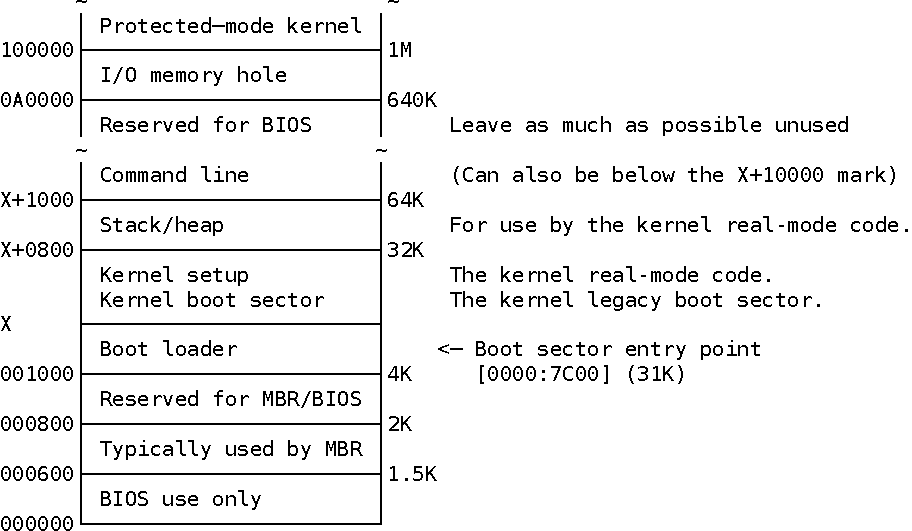
\includegraphics[width=\textwidth]{boot-mem2}
% %   \end{center}
% %   \scriptsize{where the address X is as low as the design of the boot loader permits}
% % \end{frame}

% \begin{frame}{RAM contents after boot loader is done}
%   \mode<beamer>{
%     \begin{center}
%       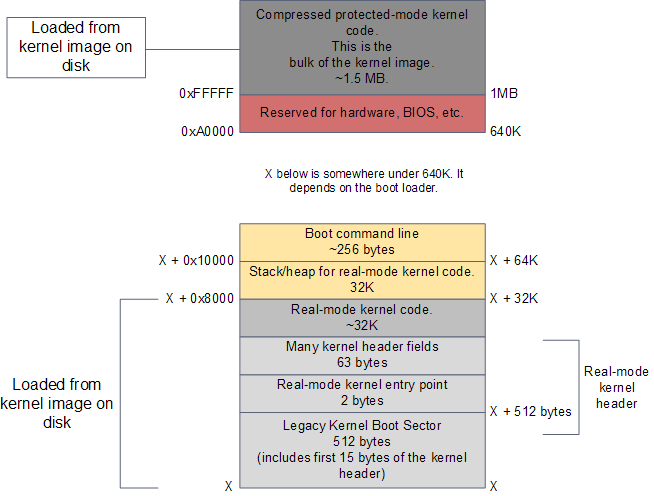
\includegraphics[width=.9\textwidth]{memoryAfterBootloader}
%     \end{center}
%   }
%   \mode<article>{
%     \begin{center}
%       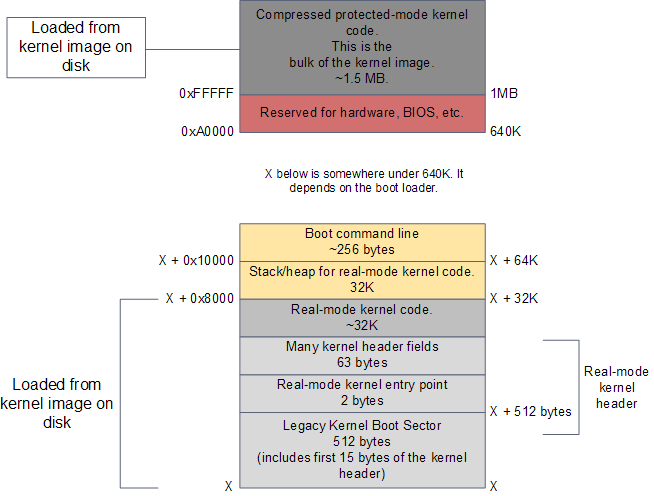
\includegraphics[width=.8\textwidth]{memoryAfterBootloader}
%     \end{center}
%   }
% \end{frame}

% \begin{itemize}
% \item Picture source: \cite{gustavo2008proess}, \cite{gustavo2008boot}
%   \begin{itemize}
%   \item This memory map is for 2.6.25, and not fully compatible with 2.6.11.
%   \end{itemize}
% \item More info about boot-time memory arrangement, see \cite{linux2.6.25protocol}.
% \end{itemize}

\subsection{setup()}

\begin{frame}{The \code{setup()} Function}
  boots and loads the executable image to ($0x9000\ll 4$) and jumps to ($0x9020\ll 4$)
  \begin{center}
    \mode<beamer>{
      
\includegraphics[width=\textwidth]{setup2}
    } \mode<article>{
      
\includegraphics[width=.7\textwidth]{setup2}
    }
  \end{center}
  \begin{itemize}
  \item \code{2.6.11/arch/i386/boot/setup.S}
  \item Re-initialize all the hardware devices
  \item Sets the A20 pin (turn off \emph{wrapping around})
  \item Sets up a provisional IDT and a provisional GDT %(line 792 in \code{setup.S})
    % \item the uncompressed part of the Linux kernel decompresses the compressed portion
    %   to
    %   address ($0x10000\ll 4$) (1M) and kernel initialization begins
  \item \code{PE=1, PG=0} in \code{cr0} %(line 824 in \code{setup.S})
  \item jump to \code{startup\_32()}
  \end{itemize}
\end{frame}

\begin{itemize}
\item \emph{Kernel attributes} are stored at the end of the boot block
  (1\textsuperscript{st}
  sector). (\href{http://lxr.linux.no/linux+v2.6.11/arch/i386/boot/bootsect.S#L90}{line 90 in
    \code{bootsect.S}})
\item
  \href{http://lists.kernelnewbies.org/pipermail/kernelnewbies/2011-March/001133.html}{From
    which point onwards the kernel execution starts?}
\item
  \href{http://unixbhaskar.blogspot.com/2010/03/insight-into-gnulinux-boot-process.html}{Insight
    into GNU/Linux boot process}
\item
  \href{http://linux-development-for-fresher.blogspot.com/2012/07/linux-boot-process-in-nutshell.html}{Linux
    Boot Process in a nutshell}
\item The \code{setup()} function:
  \begin{enumerate}
  \item Builds system's physical memory map
    \begin{itemize}
    \item find the amount of memory present in the system (sec 1.1 in
      \cite{abhishek2002memory}, \href{http://lxr.linux.no/linux-old+v2.4.19/arch/i386/boot/setup.S#L289}{\code{arch/i386/boot/setup.S}
        (2.4.19)}, line 289-389)
    \end{itemize}
  \item Sets the keyboard repeat delay and rate
  \item Initializes the video adapter card
  \item Reinitializes the disk controller and determines the hard disk parameters
  \item Checks for an IBM Micro Channel bus (MCA)
  \item Checks for a PS/2 pointing device (bus mouse)
  \item Checks for Advanced Power Management (APM ) BIOS support
  \item If the BIOS supports the Enhanced Disk Drive Services (EDD ), builds a table in
    RAM describing the hard disks available in the system
  \item If the kernel image was loaded low in RAM (at physical address 0x00010000), the
    function moves it to physical address \texttt{0x00001000} (was used by boot loader).
    \begin{description}
    \item[Why?] (Sec A.3, \emph{Middle Ages: the \code{setup()} Function},
      \cite{bovet2005understanding}) This step is necessary because to be able to store
      the kernel image on a floppy disk and to reduce the booting time, the kernel image
      stored on disk is compressed, and the decompression routine needs some free space to
      use as a temporary buffer following the kernel image in RAM.
      \begin{itemize}
      \item \code{BOOTSEG = 0x07C0}. This is 27K above \code{0x1000}. It was too small to
        hold the kernel image. After boot loader is done, \code{BOOTSEG (0x7C00)} is
        free. So kernel image can be stuffed here.
      \end{itemize}
    \item[Memory layout]
      (\href{http://unixbhaskar.blogspot.com/2010/03/insight-into-gnulinux-boot-process.html}{Insight into GNU/Linux Boot Process})

      \textbf{uncompressed image:} ... Later, all the kernel is moved from \code{0×10000}
      (64K) to \code{0×1000} (4K). This move overwrites BIOS data stored in RAM, so BIOS
      calls can no longer be performed. We don’t care because linux dosen’t use BIOS to
      acces the hardware. The first physical page is not touched because it is the
      so-called “zero-page”, used in handling virtual memory.  At this point,
      \code{setup.S} enters protected mode and jumps to \code{0×1000}, where the kernel
      lives. All the available memory can be accessed now, and the system can begin to
      run.

      The steps just described were once the whole story of booting when the kernel was
      small enough to fit in half a megabyte of memory --- the address range between
      \code{0×10000} and \code{0×90000}. As features were added to the system, the kernel
      became larger than half a megabyte and could no longer be moved to
      \code{0×1000}. Thus, code at \code{0×1000} is no longer the Linux kernel, instead
      the “gunzip” part of the gzip program resides at that address.

      \textbf{Compressed image [zimage]:} When the kernel is moved to \code{0×1000} (4K),
      \code{head.S} in the compressed directory is sitting at this address. It's in charge
      of gunzipping the kernel, this done by a function \code{decompress\_kernel()},
      defined in \code{compressed/misc.c}, which in turns calls \code{inflate()} which
      writes its output starting at address \code{0×100000} (1MB). High memory can now be
      accessed, because \code{setup.S} han take us to the protected mode now.  After
      decompression, \code{head.S} jumps to the actual beginning of the kernel. The
      relevant code is in \code{../kernel/head.S}. \code{head.S} (i.e., the code found at
      \code{0×100000}) can complete processor initialization and call
      \code{start\_kernel()}.

      The boot steps shown above rely on the assumption that the compressed kernel can fit
      in half a megabyte of space. While this is true most of the time, a system stuffed
      with device drivers might not fit into this space. For example, kernels used in
      installation disks can easily outgrow the available space. To solve this problem
      problem bzImage kernel images were introduced.

      \textbf{Big Compressed Image [bzImage]:} This kind of kernel image boots similarly
      to zImage, with a few changes.

      When the system is loaded at \code{0×10000} (64K) a special helper routine is called
      which does some special BIOS calls to move the kernel to \code{0×100000}
      (1Mb). \code{setup.S} doesn’t move the system back to \code{0×1000} (4K) but, after
      entering protected mode, jumps instead directly to address \code{0×100000} (1MB) where data
      has been moved by the BIOS in the previous step.  The decompresser found at 1MB
      writes the uncompressed kernel image into low memory until it is exhausted, and then
      into high memory after the compressed image.  The two pieces are then reassembled to
      the address \code{0×100000} (1MB). Several memory moves are needed to perform the task
      the address \code{0×100000} (1MB). Several memory moves are needed to perform the task
      correctly.
    \end{description}
    
    \begin{gascode}
      code32_start:               # here loaders can put a different
                                  # start address for 32-bit code.
      #ifndef __BIG_KERNEL__
              .long     0x1000    #   0x1000 = default for zImage
      #else
              .long     0x100000  # 0x100000 = default for big kernel
      #endif
    \end{gascode}
    \clearpage
    The default value of \code{code32} is \code{\_\_BOOT\_CS:0x1000} (\code{\_\_BOOT\_CS}
    = 16). (\href{http://lxr.linux.no/linux+v2.6.11/arch/i386/boot/setup.S#L855}{Line
      855-857})
    
    \begin{gascode}
      code32: .long 0x1000    # will be set to 0x100000 for big kernels
      .word __BOOT_CS
    \end{gascode}

    It will be changed to
    \code{\_\_BOOT\_CS:0x100000}. (\href{http://lxr.linux.no/linux+v2.6.11/arch/i386/boot/setup.S#L594}{Line
      594-595})
    
    \begin{gascode}
      movl %cs:code32_start, %eax
      movl %eax, %cs:code32
    \end{gascode}
    \code{\%cs:code32\_start} $\Rightarrow$ \code{\%cs:code32} = \code{0x10:0x100000} (for
    load high, i.e. bzImage)
\item Sets the \href{http://en.wikipedia.org/wiki/A20_line}{\code{A20}} pin located on
    the 8042 keyboard controller (for switching to pmode)
  \item Sets up a provisional
    \href{http://en.wikipedia.org/wiki/Interrupt_descriptor_table}{Interrupt Descriptor
      Table (IDT)} and a provisional
    \href{http://en.wikipedia.org/wiki/Global_Descriptor_Table}{Global Descriptor Table
      (GDT)}.
    \begin{itemize}
    \item \href{http://lxr.linux.no/linux+v2.6.11/arch/i386/boot/setup.S#L792}{line 792 in
        \code{setup.S}}
    \item \href{http://lxr.linux.no/linux+v2.6.11/include/asm-i386/segment.h#L83}{line 83-89 in \code{include/asm-i386/segment.h}}
    \end{itemize}
    The provisional GDT is created with 2 useful entries, each covering the whole 4GB
    address space \cite{abhishek2002memory}. The code that loads the GDT is:
    \begin{gascode}
      xorl %eax, %eax # Compute gdt_base
      movw %ds, %ax   # (Convert %ds:gdt to a linear ptr)
      shll $4, %eax
      addl $gdt, %eax
      movl %eax, (gdt_48+2)
      lgdt gdt_48     # load gdt with whatever is appropriate
    \end{gascode}
\begin{itemize}
\item \code{\%ds = \%cs = SETUPSEG = 0x9020}
\item \code{\$gdt} --- beginning address of the GDT table (somewhere offsetting in
  \code{\%ds}). Its actual value will be determined at assemble time by the assembler (p24
  in \cite{bartlett2009programming})
\item \code{gdt\_48}: a label in \code{setup.S}
  (\href{http://lxr.linux.no/linux+v2.6.11/arch/i386/boot/setup.S#L1006}{line
    1006}). \code{gdt\_48+2} will be filled with the \emph{gdt base} computed above.
\item \code{lgdt}: loads the value in \code{gdt\_48} into \code{GDTR}
\item \code{gdt\_48 = limit,base} $\Rightarrow$ \code{GDTR}
  \begin{itemize}
  \item \code{limit = gdt\_end - gdt - 1 = 31} (16 bits)
  \item \code{base = \%ds $\ll$ 4 + gdt} (32 bits)
  \end{itemize}
\end{itemize}
\begin{gascode}
gdt_48:
     .word      gdt_end - gdt - 1   # gdt limit
     .word      0, 0                # gdt base (filled in later)

gdt:
     .fill GDT_ENTRY_BOOT_CS,8,0

     .word      0xFFFF   # 4Gb - (0x100000*0x1000 = 4Gb)
     .word      0        # base address = 0
     .word      0x9A00   # code read/exec
     .word      0x00CF   # granularity = 4096, 386
                         #  (+5th nibble of limit)

     .word      0xFFFF   # 4Gb - (0x100000*0x1000 = 4Gb)
     .word      0        # base address = 0
     .word      0x9200   # data read/write
     .word      0x00CF   # granularity = 4096, 386
                         #  (+5th nibble of limit)
gdt_end:
\end{gascode}
\begin{itemize}
\item \code{gdt}: the provisional GDT has 4 entries.
  \begin{itemize}
  \item The 1\textsuperscript{st} and 2\textsuperscript{nd} entries are initialized to
    0\footnote{\code{.fill REPEAT,SIZE,VALUE}}
    (\href{http://lxr.linux.no/linux+v2.6.11/arch/i386/boot/setup.S#L983}{line 983}), as
    required by Intel.
    \begin{center}
      \code{.fill GDT\_ENTRY\_BOOT\_CS,8,0}
    \end{center}
  \item 3\textsuperscript{rd} is \code{\_\_BOOT\_CS}
  \item 4\textsuperscript{th} is \code{\_\_BOOT\_DS}
  \end{itemize}
  (\href{http://www.tldp.org/HOWTO/Linux-Init-HOWTO-3.html}{Linux HOWTO: Prepare to move
    to protected mode}) Calculate the linear base address of the kernel GDT (table) and
  load the GDT pointer register with its base address and limit.
  \begin{figure}[h]
    \centering
    \includegraphics[width=.3\textwidth]{gdt-boot}
    \caption{Provisional GDT in RAM}
    \label{fig:gdt-boot}
  \end{figure}
  \begin{itemize}
  \item This early kernel GDT describes kernel code as 4 GB, with base address 0,
    code/readable/executable, with granularity of 4 KB.
    \begin{figure}[h]
      \centering
      \includegraphics[width=.6\textwidth]{gdt-entry-cs}
      \caption{Code segment descriptor value: \texttt{0x00CF9A000000FFFF}}
      \label{fig:cs}
    \end{figure}
  \item The kernel data segment is described as 4 GB, with base address 0,
    data/readable/writable, with granularity of 4 KB.
    \begin{figure}[h]
      \centering
      \includegraphics[width=.6\textwidth]{gdt-entry-ds}
      \caption{Data segment descriptor value: \texttt{0x00CF92000000FFFF}}
      \label{fig:ds}
    \end{figure}
  \end{itemize}
\end{itemize}
  \item Resets the floating-point unit (FPU), if any.
  \item Reprograms the Programmable Interrupt Controllers (PIC) to mask all interrupts,
    except IRQ2 which is the cascading interrupt between the two PICs.
  \item Switches the CPU from Real Mode to Protected Mode by setting the \code{PE} bit in
    the \code{cr0} status register. The \code{PG} bit in the \code{cr0} register is
    cleared, so paging is still
    disabled. (\href{http://lxr.linux.no/linux+v2.6.11/arch/i386/boot/setup.S#L832}{line
      832-833})
\begin{gascode}
  movw $1, %ax # protected mode (PE) bit
  lmsw %ax     # This is it!
\end{gascode}
    \begin{itemize}
    \item \code{lmsw} --- \href{http://www.fermi.mn.it/linux/quarta/x86/lmsw.htmlink}{Load
        Machine Status Word} (part of \code{cr0})
    \item in later kernel (e.g. 2.6.34) the switching code is like this (\href{http://lxr.linux.no/linux+v2.6.34/arch/x86/boot/pmjump.S#L39}{line 39-41 in pmjump.S}):
\begin{gascode}
  movl %cr0, %edx
  orb $X86_CR0_PE, %dl # Protected mode
  movl %edx, %cr0
\end{gascode}
      \href{http://lxr.linux.no/linux+v2.6.34/arch/x86/include/asm/processor-flags.h#L29}{line
      29 in \code{processor-flags.h}}:
    \begin{center}
      \code{\#define X86\_CR0\_PE 0x00000001}
    \end{center}
  \end{itemize}
  \textbf{NOTE:} We are now in 32-bit protected mode. From now on, the address translation will be
  done by looking up the GDT table.
  \item Jumps to the \code{startup\_32()} assembly language function. (\href{http://lxr.linux.no/linux+v2.6.11/arch/i386/boot/setup.S#L854}{line 854})
    \begin{gascode}
        .byte 0x66, 0xea   # prefix + jmpi-opcode
code32: .long   0x1000     # will be set to 0x100000
                           # for big kernels
        .word   __BOOT_CS
      \end{gascode}
\begin{itemize}
\item \code{jmpi 0x100000,\_\_BOOT\_CS} (far jump)
  \begin{itemize}
  \item jump to \code{0x10:0x100000} (segment number: \code{0x10}; offset: \code{0x100000}.)
  \end{itemize}
\item
  (\href{http://unixbhaskar.blogspot.com/2010/03/insight-into-gnulinux-boot-process.html}{Insight
    into GNU/Linux boot process}) At the end of the initial assembly code in
  \code{arch/i386/boot/setup.S} a jump to offset \code{0x100000} in segment
  \code{KERNEL\_CS} is called. This is where the version of \code{startup\_32()} found in
  \code{arch/i386/boot/compress-ed/head.S}. But the jump is a little tricky, as we haven’t
  yet reloaded the \code{CS} register, the default size of the target offset still is 16
  bit. However, using an operand prefix (\code{0×66}), the CPU will properly take our 48
  bit far pointer [\code{.byte 0x66, 0xea}].
\end{itemize}
  \end{enumerate}
\end{itemize}


% \begin{frame}{The real-mode kernel header}
%   The action starts in \emph{the real-mode kernel header}
%   \begin{itemize}
%   \item This region of memory is used to implement the Linux boot protocol between the
%     boot loader and the kernel
%   \item \emph{Documentation/i386/boot.txt}
%   \end{itemize}
% \end{frame}

% \begin{frame}{The real-mode kernel header}
%   \begin{block}{\emph{arch/i386/boot/bootsect.S}}
%     \begin{center}
%       \includegraphics[width=.7\textwidth]{kernel-header}
%     \end{center}
%   \end{block}
%   \cfbox{red}{hd -n512 /boot/vmlinuz-x.x.x-x-x}
% \end{frame}

\subsection{startup\_32()}

\begin{frame}{\code{setup() -> startup\_32()}}%{The real mode entry point}
  \begin{block}{\code{startup\_32()} for compressed kernel}
    \begin{itemize}
    \item in \code{arch/i386/boot/compressed/head.S}
      \begin{itemize}
      \item physically at
        \begin{itemize}
        \item[]\code{0x00100000} --- load high, or
        \item[]\code{0x00001000} --- load low
        \end{itemize}
      \item does some basic register initialization
      \item \code{decompress\_kernel()}
      \end{itemize}
    \item the uncompressed kernel image has overwritten the compressed one starting at 1MB
    \item jump to the protected-mode kernel entry point at 1MB of RAM ($0×10000\ll 4$)
      \begin{itemize}
      \item \code{startup\_32()} for real kernel
      \end{itemize}
    \end{itemize}
  \end{block}
\end{frame}

\begin{itemize}
\item Initializing registers
  (\href{http://lxr.linux.no/linux+v2.6.11/arch/i386/boot/compressed/head.S#L31}{line 31
    in \code{head.S}})

  \begin{varwidth}{.3\textwidth}
    \begin{gascode}
startup_32:
        cld
        cli
        movl $(__BOOT_DS),%eax
        movl %eax,%ds
        movl %eax,%es
        movl %eax,%fs
        movl %eax,%gs

        lss stack_start,%esp
    \end{gascode}
  \end{varwidth}
    \begin{itemize}
  \item \code{cld}: clear direction flag
  \item \code{cli}: clear interrupt flag
  \item \code{lss stack\_start,\%esp}: load \code{\%ss} and \code{\%esp} pair
    (\code{\%ss:\%esp}) in a single instruction using the value stored in
    \code{stack\_start}.
    (\href{http://lxr.linux.no/linux+v2.6.11/arch/i386/boot/compressed/head.S#L40}{line 40
      in \code{head.S}})
    \begin{itemize}
    \item \code{lss} --- read a full pointer from memory and store it in the selected
      segment register:register pair. (p332, \cite{intel86})
    \end{itemize}
    % load values stored in \code{stack\_start} into \code{ss:esp}
  \item \code{stack\_start}
    (\href{http://lxr.linux.no/linux+v2.6.11/arch/i386/boot/compressed/misc.c#L296}{line
      296-303 in \code{misc.c}})

    \begin{ccode}
      struct {
        long * a;
        short b;
      } stack_start = { & user_stack [STACK_SIZE] , __BOOT_DS };
    \end{ccode}
  \item \code{STACK\_SIZE} = 4096
  \item \code{\_\_BOOT\_DS} = 24 (segment selector) $\Rightarrow$ \code{\%ss}
    \begin{itemize}
    \item the 4\textsuperscript{th} (2\textsuperscript{nd} non-zero) entry in provisional
      GDT (sec 1.2 in \cite{abhishek2002memory}). Each entry is 8 bytes.
    \end{itemize}
  \item \code{\&user\_stack[4096]} $\Rightarrow$ \code{\%esp}
  \end{itemize}
\item Clear BSS (line 55 in
  \href{http://lxr.linux.no/linux+v2.6.11/arch/i386/boot/compressed/head.S#L55}{head.S})

  \begin{varwidth}{.2\textwidth}
    \begin{gascode}
xorl %eax,%eax
movl $_edata,%edi
movl $_end,%ecx
subl %edi,%ecx
cld
rep
stosb
    \end{gascode}
  \end{varwidth}
  \begin{itemize}
  \item \href{http://www.cs.ubbcluj.ro/~dadi/ac/doc/ng1d5fc.html}{\code{stosb}} copies the
    value in \code{AL} into the location pointed to by \code{ES:DI}. \code{DI} is then
    incremented (if the direction flag is cleared) or decremented (if the direction flag
    is set), in preparation for storing \code{AL} in the next location.
  \item \code{rep} --- repeat
  \item
    (\href{http://stackoverflow.com/questions/3818856/what-does-this-assembly-do}{Stackoverflow:
      What does \code{rep stos} do?}) For \code{ecx} repetitions, stores the contents of
    \code{eax} into where \code{edi} points to, incrementing or decrementing \code{edi}
    (depending on the direction flag) by 4 bytes each time. Normally, this is used for a
    memset-type operation.

    Usually, that instruction is simply written \code{rep stosd}. Experienced assembly
    coders know all the details mentioned above just by seeing that. :-)

    ETA for completeness (thanks PhiS): Each iteration, \code{ecx} is decremented by 1,
    and the loop stops when it reaches zero. For \code{stos}, the only thing you will
    observe is that \code{ecx} is cleared at the end.
  \end{itemize}
\end{itemize}

\begin{frame}{\code{startup\_32()} for real kernel}
  \begin{block}{\code{startup\_32()} in \code{arch/i386/kernel/head.S}}
    \begin{itemize}
    \item Zeroes the kernel BSS for protected mode
    \item sets up the final GDT
    \item builds provisional kernel page tables so that paging can be turned on
    \item enables paging (\code{cr3->PGDir; PG=1} in \code{cr0})
    \item initializes a stack
    \item \code{setup\_idt()} --- creates the final interrupt descriptor table
    \item \code{gdtr->GDT; idtr->IDT}
    \item \code{start\_kernel()}
    \end{itemize}
  \end{block}
\end{frame}

\begin{itemize}
\item Sets up the final GDT
  (line \href{http://lxr.linux.no/linux+v2.6.11/arch/i386/kernel/head.S#L63}{63},
  \href{http://lxr.linux.no/linux+v2.6.11/arch/i386/kernel/head.S#L303}{303},
  \href{http://lxr.linux.no/linux+v2.6.11/arch/i386/kernel/head.S#L448}{448-450},
  \href{http://lxr.linux.no/linux+v2.6.11/arch/i386/kernel/head.S#L459}{459-463},
  \href{http://lxr.linux.no/linux+v2.6.11/arch/i386/kernel/head.S#L470}{470-EOF} in \code{head.S})
    \begin{gascode}
        lgdt boot_gdt_descr - __PAGE_OFFSET

        ...
        lgdt cpu_gdt_descr
        ...
        
boot_gdt_descr:
        .word __BOOT_DS+7                     # limit (31, end of DS)
        .long boot_gdt_table - __PAGE_OFFSET  # base location

ENTRY(boot_gdt_table)
        .fill GDT_ENTRY_BOOT_CS,8,0
        .quad 0x00cf9a000000ffff    # kernel 4GB code at 0x00000000 
        .quad 0x00cf92000000ffff    # kernel 4GB data at 0x00000000 

cpu_gdt_descr:
        .word GDT_ENTRIES*8-1
        .long cpu_gdt_table

        .fill NR_CPUS-1,8,0             # space for the other GDT descriptors
        
ENTRY(cpu_gdt_table)
        ...
        # Entry 12-15 
        .quad 0x00cf9a000000ffff    # 0x60 kernel 4GB code at 0x00000000 
        .quad 0x00cf92000000ffff    # 0x68 kernel 4GB data at 0x00000000 
        .quad 0x00cffa000000ffff    # 0x73 user 4GB code at 0x00000000 
        .quad 0x00cff2000000ffff    # 0x7b user 4GB data at 0x00000000 
        ...
      \end{gascode}
    \begin{itemize}
    \item \code{.fill REPEAT, SIZE, VALUE}
      \begin{itemize}
      \item \code{.fill 2,8,0} fills the 1\textsuperscript{st} and 2\textsuperscript{nd}
        entry with \code{0}
      \end{itemize}
    \item \code{.quad} 8-byte datas (the 3\textsuperscript{rd} and 4\textsuperscript{th}
      entry)
    \item The addresses of \code{boot\_gdt\_table} and \code{cpu\_gdt\_table} will be
      assigned by assembler at compile time.
    \end{itemize}
  \item Zeroes the kernel BSS (line 74-79 in \code{arch/i386/kernel/head.S})
      \begin{gascode}
        xorl %eax,%eax
        movl $__bss_start - __PAGE_OFFSET,%edi
        movl $__bss_stop - __PAGE_OFFSET,%ecx
        subl %edi,%ecx
        shrl $2,%ecx
        rep ; stosl
      \end{gascode}
    \begin{itemize}
    \item \code{subl \%edi, \%ecx} --- get BSS size, put into \code{\%ecx}
    \item \code{shrl \$2,\%ecx} --- \code{$\frac{\%ecx}{4}$}, get number of 4-byte chunks
      (repeat times)
    \item
      \href{http://pdos.csail.mit.edu/6.828/2004/readings/i386/STOS.htm}{\code{stosl}/\code{stosd}}
      --- Store \code{EAX} in dword \code{ES:EDI}, update \code{EDI}
    \end{itemize}
\item Initialize page tables (Sec 2.5.5, \emph{Kernel Page Tables}, \cite{bovet2005understanding})
  \begin{itemize}
  \item In the first phase, the kernel creates a limited address space including the
    kernel's code and data segments, the initial Page Tables, and 128 KB for some dynamic
    data structures. This minimal address space is just large enough to install the kernel
    in RAM and to initialize its core data structures.
  \item The provisional Page Global Directory is contained in the \code{swapper\_pg\_dir}
    variable. \code{swapper\_pg\_dir} is at the beginning of BSS (uninitialized data area)
    because BSS is no longer used after system start up.
  \item The provisional Page Tables are stored starting from \code{pg0}, right after the
    end of the kernel's uninitialized data segments (\code{\_end}).
  \item For the sake of simplicity, let's assume that the kernel's segments, the
    provisional Page Tables, and the 128 KB memory area fit in the first 8 MB of RAM. In
    order to map 8 MB of RAM, two Page Tables are required.
  \item The objective of this first phase of paging is to allow these 8 MB of RAM to be
    easily addressed both in real mode and protected mode.
    \begin{center}
      \includegraphics[width=.4\textwidth]{kernel-page-table-boot}
    \end{center}
    Therefore, the kernel must create a mapping from both the linear addresses
    \code{0x00000000} through \code{0x007fffff} (8M) and the linear addresses
    \code{0xc0000000} through \code{0xc07fffff} (8M) into the physical addresses
    \code{0x00000000} through \code{0x007fffff}. In other words, the kernel during its
    first phase of initialization can address the first 8 MB of RAM by either linear
    addresses identical to the physical ones or 8 MB worth of linear addresses, starting
    from \code{0xc0000000}.
    \begin{description}
    \item[Why?] (Sec 1.3.2, \emph{Provisional Kernel Page Tables}, \cite{abhishek2002memory})
      \begin{itemize}
      \item All pointers in the compiled kernel refer to addresses $> PAGE\_OFFSET$. That
        is, the kernel is linked under the assumption that its base address will be
        \code{start\_text} (I think; I don't have the code on hand at the moment), which
        is defined to be $PAGE\_OFFSET+(some\ small\ constant,\ call\ it\ C)$.
      \item All the kernel bootstrap code (mostly real mode code) is linked assuming that
        its base address is $0+C$.
      \end{itemize}

      \code{head.S} is part of the bootstrap code. It's running in protected mode with
      paging turned off, so all addresses are physical. In particular, the instruction
      pointer is fetching instructions based on physical address. The instruction that
      turns on paging (\code{movl \%eax, \%cr0}) is located, say, at some physical address
      \code{A}.

      As soon as we set the paging bit in \code{cr0}, paging is enabled, and starting at
      the very next instruction, all addressing, including instruction fetches, pass
      through the address translation mechanism (page tables). IOW, all address are
      henceforth virtual. That means that
      \begin{enumerate}
      \item We must have valid page tables, and
      \item Those tables must properly map the instruction pointer to the next instruction
        to be executed.
      \end{enumerate}
      That next instruction is physically located at address \code{A+4} (the address
      immediately after the "\code{movl \%eax, \%cr0}" instruction), but from the point of
      view of all the kernel code --- which has been linked at \code{PAGE\_OFFSET} ---
      that instruction is located at virtual address \code{PAGE\_OFFSET+(A+4)}. Turning on
      paging, however, does not magically change the value of EIP \footnote{The value of
        EIP is still physically \code{A+4}, not \code{PAGE\_OFFSET+(A+4)} yet. But since
        paging is just enabled, CPU could pass \code{A+4} through address translation.}.
      The CPU fetches the next instruction from ***virtual*** address \code{A+4}; that
      instruction is the beginning of a short sequence that effectively relocates the
      instruction pointer to point to the code at \code{PAGE\_OFFSET+A+(something)}.

      But since the CPU is, for those few instructions, fetching instructions based on
      physical addresses ***but having those instructions pass through address
      translation***, we must ensure that both the physical addresses and the virtual
      addresses are :
      \begin{enumerate}
      \item Valid virtual addresses, and
      \item Point to the same code.
      \end{enumerate}
      That means that at the very least, the initial page tables must
      \begin{enumerate}
      \item map virtual address \code{PAGE\_OFFSET+(A+4)} to physical address
        \code{(A+4)}, and must
      \item map virtual address \code{A+4} to physical address \code{A+4}.
      \end{enumerate}
      This dual mapping for the first 8MB of physical RAM is exactly what the initial page
      tables accomplish. The 8MB initally mapped is more or less arbitrary. It's certain
      that no bootable kernel will be greater than 8MB in size. The identity mapping is
      discarded when the MM system gets initialized.
    \end{description}
  \end{itemize}
  \begin{center}
    \includegraphics[width=.5\textwidth]{kernel-page-table}
  \end{center}
  line \href{http://lxr.linux.no/linux+v2.6.11/arch/i386/kernel/head.S#L91}{91-111} in
  \code{head.S}
    \begin{gascode}
page_pde_offset = (__PAGE_OFFSET >> 20);

        movl $(pg0 - __PAGE_OFFSET), %edi
        movl $(swapper_pg_dir - __PAGE_OFFSET), %edx
        movl $0x007, %eax                # 0x007 = PRESENT+RW+USER 
10:
        leal 0x007(%edi),%ecx            # Create PDE entry 
        movl %ecx,(%edx)                 # Store identity PDE entry 
        movl %ecx,page_pde_offset(%edx)  # Store kernel PDE entry 
        addl $4,%edx
        movl $1024, %ecx
11:
        stosl
        addl $0x1000,%eax
        loop 11b
        # End condition: we must map up to and including INIT_MAP_BEYOND_END 
        # bytes beyond the end of our own page tables; the +0x007 is the attribute bits 
        leal (INIT_MAP_BEYOND_END+0x007)(%edi),%ebp
        cmpl %ebp,%eax
        jb 10b
        movl %edi,(init_pg_tables_end - __PAGE_OFFSET)
      \end{gascode}
    \begin{center}
      \includegraphics[width=.5\textwidth]{i386pte}
    \end{center}
    \begin{itemize}
      % \item The identity mapping is discarded when the MM system gets initialized.
    \item \mint{gas}|page_pde_offset = (__PAGE_OFFSET >> 20); # 0xC00, the 3K point.|

      The \code{PGDir} is one page (4K) in size. It's divided into two parts:
      \begin{enumerate}
      \item first 3K (768 entries) for user mode
      \item last 1K (256 entries) for kernel mode
      \end{enumerate}
    \item \code{\$(pg0 - \_\_PAGE\_OFFSET)} yields the physical address of \code{pg0}
      since here it is a linear address. Same case for \code{\$(swapper\_pg\_dir -
        \_\_PAGE\_OFFSET)}.
      \begin{itemize}
      \item \code{swapper\_pg\_dir} starts at the beginning of BSS
      \item \code{pg0} starts at \code{\_end}
      \end{itemize}
    \item Registers:
      \begin{description}
      \item[\code{\%edi}] address of each page table entry, i.e. \code{pg0[0]..pg0[1023]},
        \code{pg1[0]..pg1[1023]}.
      \item[\code{\%edx}] address of \code{swapper\_pg\_dir[0]}, and then to
        \code{swapper\_pg\_dir[1]}.
      \item[\code{\%ecx}] has two uses
        \begin{enumerate}
        \item contents of \code{swapper\_pg\_dir[0]}, \code{swapper\_pg\_dir[1]},
          \code{swapper\_pg\_dir[768]},\\ \code{swapper\_pg\_dir[769]}.
        \item loop counter (1024 -> 0)
        \end{enumerate}
      \item[\code{\%eax}] \code{7, 4k+7, 8k+7 ... 8M-4k+7} for 2k page table entries in
        \code{pg0} and \code{pg1} respectively.
      \item[\code{\%ebp}] \code{= 128k + 7 + \&pg0[1023]} in the first round of loop. Its
        value cannot be determined at coding time, because the address of \code{pg0} is
        not known until compile/link time.
      \end{description}
    \item \code{stosl}: stores the contents of EAX at the address pointed by \code{EDI},
      and increments \code{EDI}. Equivalent to:
      \begin{enumerate}
      \item \code{movl \%eax, (\%edi)}
      \item \code{addl \$4, \%edi}
      \end{enumerate}
    \item \code{cmpl, jb}: if \code{\%eax} < \code{\%ebp}, jump to 10;
      \begin{itemize}
      \item \code{jb}:
        (\href{http://en.wikipedia.org/wiki/X86_assembly_language#Program_flow}{Wikipedia:
          x86 assembly language}) jump on below/less than, unsigned
      \item At the end of the 1\textsuperscript{st} round of loop, the value of
        \code{\%eax} is \code{4M-4k+7}, while the value of \code{\%ebp} depends on the
        address of \code{pg0}.

        If the kernel image is small enough (e.g. a \texttt{zImage}), \code{pg0} could be
        low enough to let the 128KB covered without a \code{pg1}.
      \end{itemize}
    \item \code{INIT\_MAP\_BEYOND\_END}: 128KB, used as a bitmap covering all pages. For
      1M pages (4GB RAM), we need 1M bits (128K
      bytes). (\url{http://kerneldiy.com/blog/?p=201})
    \end{itemize}
    \href{http://www.eefocus.com/article/09-04/71517s.html}{Equivalent pseudo C code}:
    \begin{center}
      \includegraphics[width=.7\textwidth]{provisional-pgdir1}
    \end{center}
\item
  \href{http://tldp.org/HOWTO/Linux-i386-Boot-Code-HOWTO/kernel_head.html#enable_paging}{Linux
    HOWTO: Enable paging}
  (\href{http://lxr.linux.no/linux+v2.6.11/arch/i386/kernel/head.S#L186}{line 186-194 in
    \code{head.S}})
  \begin{center}
    \includegraphics[width=.7\textwidth]{head6}
  \end{center}
\end{itemize}
    
% \begin{frame}{start\_of\_setup}
%   \begin{itemize}
%   \item sets up a stack
%   \item zeroes the bss segment
%   \item jumps to \code{main()} in \emph{arch/x86/boot/main.c}
%   \end{itemize}
% \end{frame}

% \begin{frame}{main()}
%   \code{main()} does some house keeping like detecting memory layout, setting a video mode,
%   etc. It then calls \code{go\_to\_protected\_mode()} in \emph{arch/x86/boot/pm.c}
% \end{frame}

% \begin{frame}{go\_to\_protected\_mode()}
%   \begin{itemize}
%   \item \code{enable\_a20()} --- addressing more than 1MB in real mode
%   \item \code{setup\_idt()}
%     \begin{itemize}
%     \item in real mode the \emph{interrupt vector table} is at address 0
%     \item in protected mode, let IDTR take care of it.
%     \end{itemize}
%   \item \code{setup\_gdt()} --- put GDT's address into GDTR.
%     \begin{itemize}
%     \item GDT is used for address translation (logical $\rightarrow$ linear) in protected mode
%     \end{itemize}
%   \item \code{protected\_mode\_jump()} in \emph{arch/x86/boot/pmjump.S}
%     \begin{itemize}
%     \item setting the PE (Protected Enabled) bit in the CR0 CPU register
%     \item jumping to the 32-bit kernel entry point (\code{startup\_32()} for compressed kernel)
%     \end{itemize}
%   \end{itemize}
% \end{frame}

\subsection{start\_kernel()}
\label{sec:start_kernel}

\begin{frame}
  \begin{block}{\code{start\_kernel()} --- a long list of calls to initialize various
      kernel subsystems and data structures}
    \begin{itemize}
    \item \code{sched\_init()} --- scheduler
    \item \code{build\_all\_zonelists()} --- memory zones
    \item \code{page\_alloc\_init()}, \code{mem\_init()} --- buddy
      system
    \item \code{trap\_init()}, \code{init\_IRQ()} --- IDT
    \item \code{time\_init()} --- time keeping
    \item \code{kmem\_cache\_init()} --- slab allocator
    \item \code{calibrate\_delay()} --- CPU clock
    \item \code{kernel\_thread()} --- The kernel thread for process 1
    \item login prompt
    \end{itemize}
  \end{block}
\end{frame}

% \begin{frame}{\code{rest\_init()}}
%   \code{rest\_init()} in \emph{init/main.c}
%   \begin{itemize}
%   \item \code{kernel\_thread()}
%     \begin{itemize}
%     \item \code{kernel\_thread()} $\rightarrow$ \code{kernel\_init()} $\rightarrow$ \code{init\_post()}
%       \begin{itemize}
%       \item \code{kernel\_init()} is responsible for initializing the remaining CPUs in the system
%       \item \code{init\_post()} tries to execute a user-mode process --- init starts running as
%         PID 1.
%       \end{itemize}
%     \item \code{schedule()}
%     \item \code{cpu\_idle()}
%     \end{itemize}
%   \end{itemize}
% \end{frame}

\begin{frame}{The Kernel Boot Process}
  \begin{center}
    \mode<beamer>{
      \includegraphics[height=.9\textheight]{bootprocess}
    }
    \mode<article>{
      \includegraphics[height=.5\textheight]{bootprocess}
    }
  \end{center}
\end{frame}

\begin{frame}{The Kernel Boot Process (I)}
  \begin{center}
    \mode<beamer>{
      \includegraphics[width=\textwidth]{kernelInitPartOne}
    }
    \mode<article>{
      \includegraphics[width=.8\textwidth]{kernelInitPartOne}
    }
  \end{center}
\end{frame}

\begin{itemize}
\item This picture is not fully compatible with 2.6.11.
\end{itemize}

\begin{frame}{The Kernel Boot Process (II)}
  \begin{center}
    \mode<beamer>{
      \includegraphics[width=\textwidth]{kernelInitPartTwo}
    }
    \mode<article>{
      \includegraphics[width=.8\textwidth]{kernelInitPartTwo}
    }
  \end{center}
\end{frame}

\begin{itemize}
\item This picture is not fully compatible with 2.6.11.
\end{itemize}


% \begin{frame}[allowframebreaks]
%   \mode<beamer>{
%     \frametitle{References}
%     \input{boot-a.bbl}
%   }
%   \mode<article>{
%     \bibliographystyle{unsrt}
%     \bibliography{os}
%   }
% \end{frame}

\end{document}


%   }
%   \mode<article>{
%     \bibliographystyle{unsrt}
%     \bibliography{os}
%   }
% \end{frame}

\end{document}

